% T4 of the Transport Papers series.
% Correction (2026-09-10, mechanical pass, per Leon): rule 23 misidentified T5 as the printed-version exception. T1 is the exception at Version 3.0; every other paper, T5 included, reads Version 1.0. \date corrected accordingly (was 1.1).
% v1.1 (2026-09-10, derivation session, Fable 5.1 subagent, per rule 20,
%   series-review repair pass against series_review_2026-09-09.md).
%   Sec 3 (2.5): \bibitem{ButlerT3} given T3's full subtitle "Iterated
%   Transport, the Frozen Clock, and Second Quantisation". \date bumped to
%   Version 1.1. No body text, label or numbering changed.
%   Script: verify_T04.py 296/296. Prop 5.2 block: the shadow wall is now
%   located from the Gram (det h(tau) built as a rational function, linearity
%   in tau checked, its zero interpolated exactly and compared with -2 mu nu,
%   crossing simplicity from (det h)') instead of re-evaluating the closed
%   form; two closed-form checks replaced by two Gram checks, count unchanged.
%   Sec 8.7 norm-identity label no longer asserts "bounded norm <=> membership"
%   (Rem 8.5 denies it); Sec 9.3 label "Theorem 8.11" -> "Theorem 8.16";
%   schwarzschild_checks docstring "58 checks" -> "70".
%   Compile: pdflatex x2, 50 pages, 0 errors, 0 undefined refs, 0 multiply
%   defined, 8 overfull, no float overflow.
% 2026-09-09 addendum (interactive session with Leon, Opus 5). Two changes
%   per Leon: (1) the printed version is now 1.0 for every paper T0 to T17,
%   T5 alone at 3.0 (progress-doc rule 23); the development numbering is
%   retired from the title page and kept in this header. (2) Every reference
%   to the programme monograph is removed (rule 24), re-pointed to the series
%   where a sibling paper carries the result and otherwise restated to stand
%   alone. No mathematics, no labels and no numbering changed, so verify_T04.py
%   stands unchanged at 296/296 and was not re-run.
%   Here: the twist remark restated as "The direction of the induced twist",
%   stating which way the pairing runs rather than correcting a source; the
%   simplicity-proof and generality remarks restated; the settled conjecture
%   named the Kasner-weights conjecture of this programme at its four sites.
% v1.6 (2026-09-09, derivation session, Fable 5.1 subagent, per rule 20,
%   review-repair pass against T04_review_v1.md, same session).  Review of the
%   v1.5 prose pass: 0 BLOCKING, 1 SERIOUS, 8 NON-BLOCKING; the pass itself
%   was found faithful (no claim changed level, no defined-term collision).
%   S1: Rem 10.5's closing sentence pointed the reader at the unpublished T5
%   companion note (rule 17(b)); sentence deleted.  N1: \date bumped from
%   "Version 1.0, August 2026" to 1.6, September 2026.  N2: abstract "what
%   degenerates on Sig is a splitting" -> "what fails on Sig" (a splitting does
%   not degenerate; matches the introduction); abstract still 249 words.  N3:
%   verify_T04.py labels, comments and docstring purged of the retired
%   vocabulary (dies, death, healthy, sits, kills, weld, engine, machinery,
%   from scratch); no predicate changed; banner -> v1.6.  N4: FG paragraph
%   "of Lorentzian-shifted signature" -> "of signature (p+1,q+1)".  N5: Rem
%   6.3 "per the series' correction discipline" -> "recorded rather than
%   silently applied, per the series' practice".  N6: Position-in-the-series
%   sentence on T6 un-inverted.  N7 (SG1/SG2 search takes its three input
%   orders as literals; search itself real) and N8 (8 overfull boxes, all
%   pre-existing) left as they are.  Check count unchanged: 296/296 pass (run
%   in the cloud workspace).  COMPILE: pdflatex x2, 51 pages, 0 errors, 0
%   undefined references, 8 overfull boxes, no float overflow.  Numbering
%   frozen: aux diff against v1.4/v1.5 empty.  verify_crossrefs T04: 124/124.
%   No knock-on for any sibling found (T5's cor:weld is already "The
%   matching"; T5 Fact B.4 mirrors Prop 9.17, whose statement is unchanged).
% v1.5 (2026-09-08, prose pass, Fable 5.1 subagent, per project rule 22: mannered
%   prose replaced by literal statement, Leon's ruling to replace the recurring
%   vocabulary too).  Body only (abstract, sections, statements, proofs, captions,
%   figure labels); no mathematics, numbering, labels, citations or claims changed.
%   About 145 sentences edited.  Glossary items applied: ledger (matter/black-hole
%   sense, 3x) -> boundary mode space / count of boundary modes; price/prices/pays
%   (3x) -> cost / literal rewrite; owned/owns (6x) -> assigned to; honest (4x) ->
%   nondegenerate metric, stated, correction discipline; upstairs (1x) -> in the
%   completion; kills (3x) -> makes zero / vanishes on / sends to zero; machinery
%   (7x) -> results / constructions / methods / theory; engine (2x) -> routine;
%   sits/lives (~12x) -> is / lies / is supported; healthy (10x) -> nonvanishing
%   (eigenvalues, minors) / nondegenerate (slots, block, scales); verb "dies",
%   "death", "died" (~20x) -> degenerates / vanishes / goes to zero / fails
%   (the adjective "dying direction/line/eigenvalue/entry/axis/slot" KEPT as the
%   paper's defined name of the radical direction, used in theorem statements and
%   imported by T5/T6); mints (3x) -> produces; marching (2x) -> displaced
%   successively; consumes (4x) -> uses; verdict (2x) -> conclusion; from scratch
%   (4x) -> independently / directly / self-contained; in disguise -> under
%   another name; peel -> raise one at a time; toolkit -> primer; pinned -> fixed;
%   on the nose -> exactly; conspire -> reduce; corrupting -> changing; untouchable
%   -> unaffected; wearing -> expressed in; cure -> solution; debt -> degeneracy;
%   two faces -> seen on the two sides; not by lack of ingenuity (dropped).
%   Coordinator ruling: weld/welded/welds -> matching/matched/matches (13x, labels
%   unchanged).  KEPT as defined names: rain frame, shadow wall, wall,
%   carrier, no-attic/no-echo (T8 result names), the mod-8 clock.  Abstract 249
%   words.  COMPILE: pdflatex x2 clean, 51 pages, 0 errors, 0 undefined refs;
%   numbering unchanged (aux diff empty).  verify_T04.py untouched: 296/296 pass.
% 2026-08-31 (SECOND T6 knock-on, from the re-review of T6 v1.2): two items.
%   (a) Fact 8.25's restatement of T6 Def 5.5 dropped T6's closing "both
%   locally uniformly on the boundary base", so it asserted T6's theorem for
%   the strictly larger pointwise class; the clause is restored. (b) Rem
%   rem:bouncedyn put the Kasner map and its era structure INSIDE T6's
%   admissibility class, where T6's admissibility integral in fact diverges
%   (T6 Rem 5.8); it now places them outside it, in T6's billiard-invariant
%   successor problem. Bare \cite, so verify_crossrefs could not see either.
%   No result renumbers; compile clean; suite locators 368/368.
% 2026-08-31 (T6 review knock-on, derivation pass, per Leon's review of this
%   date): Fact 8.25's admissibility parenthetical brought up to T6 Def 5.5
%   v1.2 (Einstein hypothesis and E_tau -> 0 added; both load-bearing in T6's
%   proof), and both holonomy sentences (Fact 8.25, Thm 8.27(3)) qualified as
%   values-level per T6. No result renumbers; compile clean; suite locators
%   re-checked (verify_crossrefs T04). verify_T04.py untouched.
% v1.0 (review draft, 2026-08-20): complete. History: M1 skeleton/degeneration
% sheaf (sharpened unit-ideal proof, no simplicity needed); M2 one-sided
% completion at (p,q)-generality (exact wall Gram, exact determinant identity);
% M3 shadow wall (NEW absolute conservation theorem; quantitative good
% couplings; unconditional infinite wall sequence); M4 exceptional algebra +
% residue with the CORRECTED twist (conormal = L^2, partner = sqrt(normal));
% M5 two-sidedness corollary, choices/obstructions, wall-class conjecture,
% tractor/FG dictionary (assembly level); M6 verify_T04.py 41/41; M7 assembly.
% v1.2 (2026-08-29, per Leon: fold in the transversal/no-value results of the
%   T5 companion note "Three Routes from the Localisation").  NEW Section 10
%   "Transversal independence, and the no-value theorem at the wall",
%   inserted BEFORE "Position in the series" (which becomes Section 11, the
%   verification section 12; nothing externally cited renumbers: siblings
%   cite T4 by Secs 4, 8, 9 and result numbers 4.x/8.x only, checked).
%   Contents: Lem 10.1 (base unipotents at the wall), Lem 10.2 (the solve
%   closed by the radical gauge), Thm 10.3 (transversal independence: the
%   unipotent intertwiner Phi_v, completion canonically independent of the
%   collar transversal), Thm 10.4 (no equivariant value at the wall: the
%   automorphisms theta_lambda act on candidate values by free translations,
%   no fixed point; T1 Thm 4.2 thereby holds AT the wall, hyperbolic partner
%   absent), Rem 10.5 (scope: pointwise/smooth, constants fixed, off-wall
%   unobstructed and unneeded; discharges the boundary case T5's Fact 5.4
%   records as open).  Verification section: totals 262 -> 284, coverage
%   paragraph added (twenty-two new checks, two masses, controls included).
%   verify_T04.py: transversal_checks() appended, self-contained; 284
%   checks, all pass.  COMPILE: pdflatex x2 clean, 48 pages, no undefined
%   references (aux: sec:transversal = 10, thm:transversal = 10.3,
%   thm:novalue = 10.4).
% v1.4 (2026-08-30, per Leon: final-fixes list, items 5-7).  (5) Prop 9.17
%   strengthened to three clauses: (1) as before; NEW (2) closure of the
%   C^infty-linear class under composition, sums and function multiples,
%   tensor operations, Clifford multiplication, and passage to the named
%   submodules and quotients, so composites need no re-argument; (3) the
%   "In particular" clause disambiguated: the quantifier is over the
%   endomorphisms the constructions SUPPLY, not over all endomorphisms of
%   the supplied bundles (a differential operator on a supplied bundle's
%   sections is not C^infty-linear, and none is supplied).  Proof extended
%   accordingly.  T05's Fact B.4 mirrors the new statement.  (6) Section 10
%   surfaced above the fold: abstract gains the transversal-independence /
%   no-value sentence; Contribution list "seven clusters" -> "eight" with a
%   new item 8 for Sec 10; Position in the series now records the two
%   exports to T05 (Thm 10.4 -> Fact B.3, Prop 9.17 -> Fact B.4, cited as
%   \cite[Facts B.3, B.4]{ButlerT5}, locators verified against T05's aux).
%   (7) abstract cut 314 -> 248 words (house ceiling 250).  No result
%   numbers change; verify_T04.py unchanged except the banner -> v1.4
%   (no new computational identities; 296 checks, all pass, run in the
%   cloud workspace).  COMPILE: pdflatex x2 clean, 51 pages, no undefined
%   references, no broken cross-file locators (verify_crossrefs T04: 54/54).
%   MECHANICAL PASS ADDENDUM (2026-08-30, at T5's declare-done freeze; NO
%   mathematical change).  Sec 8's Schwarzschild provenance line now reads
%   \cite{ButlerT5}, Props.~2.2, 2.4, 2.5 and 2.6: Prop 2.4 is where T5
%   states invertibility in closed form at every r > 0, which the sentence
%   claims and 2.5 (the fold) and 2.6 (the degeneration) do not carry.
%   That locator sits OUTSIDE the \cite[...] optional argument, so
%   verify_crossrefs cannot see it; it was found by hand.  The 54/54 figure
%   above was measured before the checker was repaired (it had been counting
%   every locator into T5 as external); re-run against a fresh .aux it is
%   103/103, both directions clean.  51pp and 296/296 unchanged.
% v1.3 (2026-08-30, per Leon: apply the second-session review verdict on the
%   v1.2 Section 10).  Mathematics unchanged (Lems 10.1, 10.2, Thm 10.3 held
%   under re-derivation); the framing defects repaired.  (T04-1) the
%   "completed structure" is now DEFINED in the Sec 10 preamble as the triple
%   (T, h_u, k) with its grading and degeneration subalgebra, the named frame
%   and k* being choices inside it (with the frame retained, u is recoverable
%   as alpha(u) = 2 h_u(alpha, k*), and the theorem would not bite); Thm 10.4
%   now also proves that no theta-fixed ladder partner exists (Fix(theta_lam)
%   lies in the h_u-orthogonal of k for lam != 0) and that the construction
%   attaches partners to candidates injectively.  (T04-2) Rem 10.5's off-wall
%   isometry claim was FALSE (det h depends on the transversal through s, so
%   the shadow wall moves): replaced by the correct statement with the model
%   counterexample G = diag(lam,1,-1,-1), mu nu = 1.  (T04-3) Thm 10.3 now
%   states and proves the cocycle Phi^u_v o Phi^(u+v)_w = Phi^u_(v+w) (this is
%   what "canonically" means), says independence is an at-the-wall statement,
%   and records what Phi_v does and does not preserve (form, grading,
%   degeneration subalgebra preserved; Phi_v(k*) = k* + vtilde/2, Phi_v(sigma)
%   = sigma + vtilde k).  (T04-4) "with collar data fixed" -> "with the collar
%   constants mu, nu and the bump held fixed" (collar data include u itself).
%   (T04-5) the transfer clause is now "an analogue of the no-repair theorem
%   ... holds at the wall itself, where the base form carries no hyperbolic
%   partner for k and that theorem's hypotheses fail".  (T04-6) "records as
%   open" -> "recorded as open".  (T04-7) Sec 12's Section-10 sentence
%   rewritten to what the script does.  (T04-10) Cor 8.20 given its one-line
%   proof from Thm 8.18; Cor 8.24 and Cor 9.14 demoted to Remarks (labels
%   rem:rainanswer, rem:wallcomplex; two internal refs updated; shared
%   counter, so NO numbers change).  NEW Prop 9.17 (prop:functionlinear):
%   the C^infty-linearity principle of Sec 9's head, numbered and proved so
%   that T05 can import it as a Fact (T05-13).  Inserted at the end of Sec 9,
%   after Rem 9.16; nothing renumbers.
%   verify_T04.py -> v1.3 (version string in the banner, T04-9): check 11
%   (T04-8) now DERIVES the contragredient from theta by exact inversion and
%   asserts it equals id - lambda (x) k before applying it; new checks: the
%   cocycle, a second (angular) lambda, Fix(theta) computed as a kernel and
%   shown h_u-orthogonal to k, the Clifford-level images of k* and sigma in
%   the exterior model on all 64 states, the intertwiner at mu nu > 0, and
%   the Rem 10.5 off-wall counterexample.  284 -> 296 checks, all pass
%   (run in the cloud workspace, not on Leon's machine).
%   COMPILE: pdflatex x2 clean, 50 pages, no undefined references (aux:
%   prop:functionlinear = 9.17, thm:transversal = 10.3, thm:novalue = 10.4).
%   FOR THE MECHANICAL PASS: T05 v1.18 imports Prop 9.17 as Fact B.4 and
%   re-imports Thm 10.4 verbatim as Fact B.3 (the statement changed here).
% v1.1 = figures added per house rule 13 (one figure: the wall sequence
%        marching away from the physical region, Section 5); no other changes.
% 2026-08-25 (edit requested by Leon): Section 8 added, "The Schwarzschild
%        composite": blow-up + Kasner weights execute the successor programme
%        for exact Schwarzschild (boundary-tame wall, (2,4) completion with no
%        shadow wall, weights forced = Kasner exponents, ZD Conj 5.8 settled in
%        the diagonal class).  Integrated from the standalone draft note of
%        2026-08-25, now superseded.  At the same touch: tameness tags repaired
%        ((T1)/(T1)/(T2) -> (T1)/(T2)/(T3); the 2026-08-24 renumber pass had
%        caught the hypothesis labels); Position-in-the-series section added
%        per rule 15; bibkey ButlerVerifyT05 -> ButlerVerifyT04; verify_T04.py
%        extended 41 -> 99 checks; second figure (rule 13 allows two).
% 2026-08-25 (second edit requested by Leon): the theorem-complete results of
%        the open-items note folded in.  New subsections 8.6 (uniqueness of
%        the weighted module, with the eigenvalue subtlety), 8.7 (the rain
%        frame: duality with the infalling observer, the chain's dyad), 8.8
%        (the weld with T6's weighted limit, fibre and connection level);
%        new Section 9 (the anisotropic class: variable-order weights,
%        stability under relatively admissible errors, sharpness).  The Kerr
%        material of the note is NOT absorbed (it is conjecture-grade and
%        belongs to T6's orbit); the scope sections now cite the note's exact
%        Kerr structure results instead.  verify_T04.py extended 99 -> 197
%        checks (the note's non-Kerr checks ported).
% 2026-08-26 (third edit requested by Leon): the two T4-native residues of the
%        successor ledger closed.  New subsections 9.2 (the smooth structure
%        of the variable-order algebra: the log obstruction, the log
%        completion A^log, conormality, exponent ratios as the invariant, the
%        reduction no-go: variable-order polyhomogeneous at the unavoidable
%        price of logarithms) and 9.3 (exponent collisions and the edge of
%        the wall: collision census on the Kasner variety, the dichotomy
%        theorem: positive-pair collisions pass through the Schwarzschild
%        triple and are interior, ordering changes force Taub edges where the
%        wall ends and no module crosses; the mixmaster wall complex; the
%        Schwarzschild triple maximises the dying order).  Bounce dynamics and
%        the admissibility dictionary stay with T6 (deferred work orders in
%        the progress doc).  verify_T04.py extended 197 -> 244 checks.
% 2026-08-26 (fourth edit requested by Leon): self-referencing editorial
%        history removed from the body (the "original successor list ...
%        restated" framing of the What-remains-open paragraph, "successor
%        ledger" phrasings, "deferred work order" project language): the
%        paper now reads timelessly, as unpublished work should.  The
%        bibitem ButlerOpenNote (the unpublished open-items note) REMOVED
%        with both its citations; the Kerr passages now state the leading
%        structure as preliminary computation by the methods of Section 8,
%        claim-light, with the composite posed as the open successor
%        problem.  New house rule recorded in the progress doc.
% 2026-08-26 (fifth edit: fresh-agent review pass, three independent referees,
%        every finding hand-verified before application): coupling requires a
%        TRIVIAL radical line bundle (w1(L) = 0), now a stated hypothesis with
%        the twisted variant posed; conservation (located) crossing direction
%        proved via the Schur complement (det sign alone cannot exclude
%        (p+2,q)); absolute conservation restated with sig(K) constant across
%        the disconnected exterior; wall induction: Sigma compact hypothesised,
%        good-coupling zone corrected, Riesz projection replaced by an
%        adjugate/Jacobi argument, shadow radical trivialised by an explicit
%        global kernel section; ideal sheaf restated (finitely presented
%        bimodule + kernel ideal sheaf; C-infinity O is not coherent);
%        bounded-norm module definition repaired (null mixing collapses it:
%        new Remark + Example ex:nullmix, a second boundary-tame extension),
%        uniqueness restated within the rain-bounded class; weight forcing
%        restated per named dying slot; mass normalisation of the completion
%        fixed (u = dt/m, so k(u) = 1; ladder pair now correct at all masses,
%        checked at m = 1 and 2); r-conormal convention stated; log
%        obstruction non-membership proof replaced (exponent peeling; the
%        operator argument was invalid); variable-order algebra given
%        admissible-family semantics + boundary-unit inversion lemma; Fact
%        envs for classification values and line-bundle topology; T6
%        provenance corrected (Thm 5.6 + Lem 5.4, not "5.8"); Position
%        section moved before verification per rule 15; notation
%        disambiguation (Xi perturbation, ell log index, zeta unit,
%        vartheta frame). verify_T04.py extended (second-mass completion
%        block + null-mixing example checks).
% 2026-08-27 (sixth edit, requested by Leon): provenance of Fact 8.1
%        updated to T5's current numbering (the unipotent ray is now T5
%        Prop 2.2; the null-kernel failure is T5 Props 2.5 and 2.6, the
%        exact rescaled-limit form).  No other change.
% House rules: no em dashes; short abstract; standard series disclaimer.
\documentclass[11pt]{article}
\usepackage[margin=1.1in]{geometry}
\usepackage{amsmath,amssymb,amsthm,mathtools}
\usepackage[dvipsnames]{xcolor}
\usepackage{tikz}
\usepackage[colorlinks=true,linkcolor=MidnightBlue,citecolor=MidnightBlue,urlcolor=MidnightBlue]{hyperref}

\newtheorem{theorem}{Theorem}[section]
\newtheorem{proposition}[theorem]{Proposition}
\newtheorem{lemma}[theorem]{Lemma}
\newtheorem{corollary}[theorem]{Corollary}
\theoremstyle{definition}
\newtheorem{definition}[theorem]{Definition}
\newtheorem{remark}[theorem]{Remark}
\newtheorem{example}[theorem]{Example}
\newtheorem{conjecture}[theorem]{Conjecture}
\newtheorem{hypothesis}[theorem]{Hypotheses}
\newtheorem{fact}[theorem]{Fact (imported)}

\newcommand{\Cl}{\mathrm{Cl}}
\newcommand{\R}{\mathbb{R}}
\newcommand{\HH}{\mathbb{H}}
\newcommand{\Mat}{\mathrm{M}}
\newcommand{\rad}{\mathrm{rad}}
\newcommand{\shA}{\mathcal{A}}
\newcommand{\shC}{\mathcal{C}}
\newcommand{\shJ}{\mathcal{J}}
\newcommand{\shK}{\mathcal{K}}
\newcommand{\shE}{\mathcal{E}}
\newcommand{\shL}{L}
\newcommand{\id}{\mathrm{id}}
\newcommand{\Sig}{\Sigma}
\newcommand{\Mo}{M^{\circ}}
\newcommand{\Mp}{M^{+}}
\newcommand{\nO}{n_0}
\newcommand{\nInf}{n_\infty}
\newcommand{\shW}{\mathcal{W}}
\newcommand{\Mt}{\widetilde{M}}
\newcommand{\hb}{\bar{h}}
\newcommand{\dtS}{dt_{\mathrm{S}}}
\newcommand{\dtPG}{dt}

\title{\bfseries Clifford Sheaves over Degenerate Metrics\\[4pt]
  \large\itshape Nilpotent Ideals, One-Sided Completion, and the Exceptional Algebra}
\author{Leon Butler\\ \normalsize\href{mailto:lbutler.math@gmail.com}{\texttt{lbutler.math@gmail.com}}\\ \normalsize ORCID: \href{https://orcid.org/0009-0006-4449-5617}{0009-0006-4449-5617}}
\date{Version 1.0, September 2026 \textperiodcentered{} Transport Papers, T4}

\begin{document}
\maketitle

\begin{abstract}
\normalsize
Let $M$ be a smooth manifold with a cometric $G$ on $T^*M$, degenerating tamely to corank one on a hypersurface $\Sig$. The Clifford sheaf of the pair meets an apparent contradiction: locally free fibre dimension cannot jump, yet the series' transport principle demands $\Cl(p,q)$ off $\Sig$ and $\Cl(p{+}1,q{+}1)$ over it. The jump goes into structure, twice over. The degeneration sheaf has constant rank $2^n$; over $\Sig$ its fibres acquire a canonical square-zero ideal, generated by the radical line, that any nondegenerate completion converts into the unit ideal. The ambient sheaf has constant rank $2^{n+2}$ and signature $(p{+}1,q{+}1)$ on the closed physical side; what fails on $\Sig$ is a splitting, the adjoined ladder pair supported exactly there. A conservation law follows: no completion standard off the wall is nondegenerate on both sides; the degeneracy reappears on a displaced shadow wall, tame for good couplings, and the construction iterates. The normal cone carries an exceptional algebra, and the metric's residue makes the dying line a canonical square root of the conormal bundle. The completion is canonically independent of the collar transversal, yet the wall admits no equivariant value and no canonical ladder partner: the no-repair theorem's analogue at the wall itself. Blown up and Kasner-weighted, the Schwarzschild singularity becomes a boundary-tame wall receiving the same completion, no shadow wall, the weights forced to the Kasner exponents; the weighted module is the unique rain-bounded boundary-tame extension, and the theory extends, stably, to position-dependent exponents. Complete proofs; imports stated as facts with provenance.
\end{abstract}

\medskip
\noindent\textbf{MSC 2020.} Primary 15A66, 53C50; Secondary 53A30, 14E15, 58A30.\\
\textbf{Keywords.} Clifford algebra; degenerate metric; signature change; nilpotent ideal; blow-up; deformation to the normal cone; tractor calculus; ambient metric.

\newpage
\textbf{Authorship and disclosure. }The founding idea of the series is the author's: that division by zero in a Clifford algebra should be read not as a prohibition but as a transport into a higher-dimensional algebra, and that the transported division need not be accompanied by an inverse operation. The direction of investigation and the critical review of the results are likewise the author's. The mathematical development and the drafting of the text were carried out in extended collaboration with Claude Fable 5 (Anthropic), an AI system.

\newpage
\section{Introduction}\label{sec:intro}

The root paper of this series operates at a single fibre. Given a real quadratic space of mixed signature, the null vectors of its Clifford algebra admit no equivariant element-level repair in any extension, while the space of points is repaired totally and uniquely by the Witt completion $\Cl(p,q) \to \Cl(p{+}1,q{+}1)$; the full taxonomy of zero-divisor obstructions, with the transport rule and minimality theorem belonging to each type, is settled in the same paper \cite{ButlerT1}. It treats one algebra at a time.

Geometry does not. In the gravitational application that motivates the series, the metric degenerates on a \emph{locus} $\Sig$ inside a manifold $M$: the algebra that needs completion is over $\Sig$, while the algebra away from $\Sig$ is nondegenerate and must be left unchanged. The natural demand is therefore a sheaf of Clifford algebras whose fibre is $\Cl(p,q)$ on the nondegenerate region and $\Cl(p{+}1,q{+}1)$ over $\Sig$. Stated naively this is impossible, and the impossibility is instructive: $\Cl(p,q)$ has dimension $2^n$ and $\Cl(p{+}1,q{+}1)$ has dimension $2^{n+2}$ (sixteen against sixty-four in the spacetime case), and the rank of a locally free sheaf is locally constant. The fibre dimension cannot jump. The subject of this paper is the resolution of that tension: the jump must be relocated into \emph{structure}, and there are exactly two natural places for it to go.

The first is a sheaf of constant rank $2^n$, the \emph{degeneration sheaf}: the Clifford sheaf of the degenerate cometric itself. Its fibres over $\Sig$ remain $2^n$-dimensional but degenerate as algebras, acquiring a canonical two-sided ideal that squares to zero. The singular locus registers as non-reducedness, in precise parallel with the appearance of nilpotents in the special fibres of algebraic-geometric degenerations, and the ideal is exactly the kind of object a blow-up is performed along: a canonical sheaf of ideals supported on the singular locus. The second is a sheaf of constant rank $2^{n+2}$, the \emph{ambient sheaf}, whose fibre is $\Cl(p{+}1,q{+}1)$ at every point of the closed physical region; the metric-level description survives inside it as a distinguished subalgebra attached to a splitting, and on $\Sig$ it is the splitting, not the sheaf, that fails. Nothing jumps in the completion. The two sheaves are related by a global embedding, and the embedding is the localised transport.

Two further phenomena complete the picture, and both are theorems rather than constructions. First, a conservation law: the one-sided completion cannot be two-sided; no completion that is standard away from the wall is nondegenerate on both sides. The ambient form necessarily degenerates on a displaced hypersurface on the unphysical side, a \emph{shadow wall}, which for good couplings is itself a tame degeneration, so the completion iterates along an infinite wall sequence; degeneracy is moved, never destroyed. Second, an exceptional fibre: the anisotropic rescaling of the dying direction by $\sqrt{t}$ realises, fibrewise over $\Sig$, the deformation to the normal cone of algebraic geometry, and its special fibre is a genuine nondegenerate Clifford algebra whose metric in the dying direction is the \emph{rate} of the degeneration. The residue theorem then identifies the twist: the physical metric has a canonical simple pole at the wall, its residue induces an isomorphism $N^*\Sig \cong \shL^{\otimes 2}$ with $\shL$ the radical line bundle, so the dying line is a canonical square root of the conormal bundle and the Witt partner line adjoined by the completion, canonically $\shL^*$, is a canonical square root of the normal bundle. The new dimension is not adjoined arbitrarily; it is constructed tautologically from the dying direction and the geometry of its degeneration.

\subsection*{Prior art}

Ambient constructions over conformal and degenerate structures have a substantial history, and this paper's ambient sheaf is a degenerate-locus-adapted relative of two of them. \emph{Tractor calculus}, going back to Thomas and formalised by Bailey, Eastwood and Gover \cite{BEG1994} with a modern treatment by Curry and Gover \cite{CurryGover2018}, packages a conformal manifold into a rank-$(n{+}2)$ bundle of signature $(p{+}1,q{+}1)$ with canonical connection; its almost-Einstein and boundary variants are the closest existing geometry to the completion of Section \ref{sec:ambient}. The \emph{Fefferman-Graham ambient metric} \cite{FG1985, FG2012} realises the same increment $(+1,+1)$ as a nondegenerate metric on a thickened cone. The precise dictionary between those constructions and the present one is assembly-level material and is developed in Section \ref{sec:dictionary}, per the series' practice of keeping the points of contact with existing structures in the text. The algebraic input, the Clifford algebra of a \emph{degenerate} symmetric form with its $2^n$-dimensional blade basis, is due to Chevalley \cite{Chevalley1997}; the structure theory of the nondegenerate fibres is classical \cite{Porteous1995, Lounesto2001, Lam2005}. On the geometric side, the blow-up along an ideal sheaf and the non-reducedness of special fibres are standard algebraic geometry \cite{Hartshorne1977}, and the deformation to the normal cone realised fibrewise in Section \ref{sec:exceptional} is Fulton's \cite[Ch.~5]{Fulton1998}. Signature-change hypersurfaces and conformally regularised cosmological boundaries, the tame class's physical exemplars, appear throughout the literature on signature change and on Penrose's conformal cyclic cosmology \cite{Penrose2010}. None of these sources, to our knowledge, treats the degenerating \emph{Clifford} sheaf itself, its nilpotent ideal, or the conservation-of-degeneracy phenomenon; those, together with the residue identification of the twist, are the contributions claimed.

\subsection*{Contribution}

The paper proves eight clusters of results, at the standard of \cite{ButlerT1} (Tier A of the series: complete proofs, each theorem carrying its own hypotheses).

\begin{enumerate}
\item \textbf{The degeneration sheaf} (Section \ref{sec:degeneration}). For a cometric of corank one along a tame hypersurface, the Clifford sheaf $\shA = \Cl(T^*M, G)$ is locally free of constant rank $2^n$ (Proposition \ref{prop:localfree}, valid for arbitrary degeneracy); over the degenerate locus each fibre carries the canonical square-zero two-sided ideal generated by the radical line, with quotient the Clifford algebra of the induced nondegenerate form, and these ideals assemble into a coherent sheaf supported exactly on $\Sig$ (Theorem \ref{thm:degsheaf}). Resolution is characterised ideal-theoretically: in any fibrewise nondegenerate Clifford completion the radical generates the \emph{unit} ideal (Proposition \ref{prop:resolution}); completion turns an infinitesimal into a dimension. The proof given needs no simplicity hypothesis, the hyperbolic partner exhibiting the unit directly, so the statement holds in the split signatures as well.
\item \textbf{One-sided completion} (Section \ref{sec:ambient}). For walls with trivial radical line bundle (the twisted case is posed as a successor problem), a rank-$(n{+}2)$ ambient bundle with a coupled form $h$, equal to $G \perp H$ outside a collar of $\Sig$, is nondegenerate of constant signature $(p{+}1,q{+}1)$ on the closed physical side; the subalgebra generated by $T^*M$ is canonically the degeneration sheaf, globally; and the localised ladder pair exists exactly over $\Sig$.
\item \textbf{The shadow wall} (Section \ref{sec:wall}). Conservation of degeneracy in two forms. Absolute: \emph{no} completion whatever that is standard outside a neighbourhood of the wall is nondegenerate everywhere, by a pure signature obstruction (Theorem \ref{thm:absolute}), which is stronger than any ansatz-level statement. Located: within the coupling ansatz the degeneration lies exactly on the zero set of the determinant factor $F$, displaced to the unphysical side, with the signature passing from $(p{+}1,q{+}1)$ to $(p,q{+}2)$; for good couplings the shadow wall is itself tame and the infinite wall sequence iterates unconditionally (Lemma \ref{lem:wallinduction}, Corollary \ref{cor:wallsequence}). The cohomological wall-class question, and its relation to the conservation conjecture of \cite[\S7.4]{ButlerT1}, is posed precisely.
\item \textbf{The exceptional algebra and the residue} (Section \ref{sec:exceptional}). The $\sqrt{t}$-rescaled Clifford family through a tame wall converges to a nondegenerate special fibre built from normal-cone data, independent of all choices up to canonical isomorphism; the inverse cometric has a canonical simple pole at the wall whose residue is exactly the inverse of the invariant transversality datum of (T3), identifying $N^*\Sig \cong \shL^{\otimes 2}$: the dying line is a canonical square root of the conormal bundle, the partner line of the normal bundle. The identification fixes the direction of the twist (Remark \ref{rem:twistcorrection}).
\item \textbf{Topology, dictionary and scope} (Section \ref{sec:dictionary}). A topological corollary of the residue theorem: tame walls are always two-sided, since $N^*\Sig \cong \shL^{\otimes 2}$ makes the normal bundle's $w_1$ zero; the construction's global choices are itemised with their exact obstruction classes ($w_1(\shL)$ the only genuine invariant); the wall class is posed as a precise conjecture whose coarse half Theorem \ref{thm:absolute} already proves; and the relation to tractor bundles and the Fefferman-Graham ambient metric is developed at assembly level and flagged as such, with the anisotropic, higher-codimension and BKL-weight questions stated as successor problems, the first instance of which the next item executes.
\item \textbf{The Schwarzschild composite} (Section \ref{sec:schwarzschild}). The two failure modes that keep the Schwarzschild singularity outside the tame class, codimension three and anisotropy, are cleared together for the exact solution: the real oriented blow-up of the worldline absorbs the angular rates tautologically, and on a canonically weighted coframe module the residual degeneration is boundary-tame of corank one, with the Killing-time direction as its radical (Theorem \ref{thm:schwtame}). The one-sided completion then ascends $\Cl(1,3) \to \Cl(2,4)$ on the whole blown-up manifold with the ladder pair supported exactly on the singular boundary and no shadow wall (Theorem \ref{thm:schwcompletion}); the weights that achieve this are forced, once the geometrically determined dying direction is named, and equal the Kasner exponents (Theorem \ref{thm:weights}), settling the Kasner-weights conjecture for Schwarzschild in the diagonal class.
\item \textbf{Uniqueness, the rain frame, the matching, and the anisotropic class} (Sections \ref{subsec:uniqueness}-\ref{subsec:weld}, \ref{sec:anisotropic}). The weighted module is the \emph{unique} rain-bounded locally free extension of the interior cotangent module that is boundary tame, by a determinant argument whose hypothesis must be read on the dying eigenvalue, not the dying entry, and whose anchoring class cannot be dropped: two explicit modules separate the readings (Theorem \ref{thm:uniqueW}, Examples \ref{ex:eigenentry} and \ref{ex:nullmix}). Physically, the exceptional coframe is exactly the dual coframe of the infalling orthonormal frame, with exact Minkowski Gram at every radius, and the gauge field carries the flat radial null dyad onto a physical dyad with constant unit components in it (Propositions \ref{prop:raindual}, \ref{prop:dyad}): the weighted module is the $u$-smooth shadow of what the falling observer measures finitely. The weighted limit of \cite{ButlerT6} is then matched to the present construction, at the fibre and at the connection level: its adapted frame consists of exceptional-module sections, its rates are re-derived here exactly, its limit is the weight one-form of the exceptional bundle, and its surviving matrix is a unit boost precisely by the second Kasner relation (Proposition \ref{prop:fibreweld}, Theorem \ref{thm:connweld}). Finally the whole package extends to position-dependent Kasner exponents, over a variable-order function algebra, stably under the relative error structure that velocity-dominated asymptotics deliver, with sharpness exhibited at relative order zero (Theorems \ref{thm:varexp}, \ref{thm:stability}); the smooth structure of that algebra is characterised exactly, variable-order polyhomogeneous with unavoidable logarithms measured by the derivative of the exponents (Theorems \ref{thm:diffclosure}, \ref{thm:ratios}); and the mixmaster boundary is closed at the algebraic level by the collision dichotomy: positive-pair collisions pass through the Schwarzschild triple and are interior to the theory, while ordering changes force Taub edges on which the wall ends and across which no weighted module continues (Theorem \ref{thm:edge}, Remark \ref{rem:wallcomplex}).
\item \textbf{Transversal independence, and the no-value theorem at the wall} (Section \ref{sec:transversal}). The coupling uses a transversal, and the dependence is resolved exactly: a closed-form unipotent intertwiner identifies the completions built on any two transversals, the identifications compose (a cocycle), and the completion at the wall is canonically transversal-independent, preserving the form, the grading and the degeneration subalgebra though neither the frame nor the ladder pair (Theorem \ref{thm:transversal}). On the same mechanism, the wall admits no equivariant classical value for the dying direction and no canonical ladder partner: the automorphisms of the completed structure translate the candidates freely (Theorem \ref{thm:novalue}), so an analogue of the root paper's no-repair theorem holds at the wall itself, where that theorem's hypotheses fail. This is the boundary no-go the singularity paper imports verbatim.
\end{enumerate}

\section{Setup: degenerate cometrics and tameness}\label{sec:setup}

\subsection{The objects}\label{subsec:objects}

Throughout, $M$ is a smooth manifold of dimension $n \geq 2$, all data are $C^\infty$, and a \emph{cometric} on $M$ is a smooth symmetric bilinear form $G$ on the cotangent bundle $T^*M$, i.e.\ a smooth section of $S^2 TM$. We work on the cotangent side because that is where the gravitational application delivers the data: in gauge theory gravity it is the gauge field's induced cometric that crosses the singular locus smoothly while metric components diverge. Nothing below depends on that origin, and the tangent-side theory is identical under $T^*M \leftrightarrow TM$.

At a point $x$, the \emph{radical} of $G_x$ is $\rad(G_x) = \{\alpha \in T^*_xM : G_x(\alpha, \cdot) = 0\}$, and the \emph{corank} of $G_x$ is its dimension. The degenerate locus of $G$ is $\Sig = \{x : \rad(G_x) \neq 0\}$. On $M \setminus \Sig$ the form is nondegenerate and its signature is locally constant.

\begin{hypothesis}[Tameness]\label{hyp:tame}
The pair $(M, G)$ is a \emph{tame corank-one degeneration} if:
\begin{enumerate}
\item[(T1)] $\Sig$ is a smooth closed hypersurface of $M$;
\item[(T2)] $G$ has corank exactly one at every point of $\Sig$, and the radical lines assemble into a smooth line subbundle $\shL \subset T^*M|_\Sig$, locally spanned by a covector field $k$;
\item[(T3)] (transversality) the degeneration is first-order: the canonical section $\delta$ of Lemma \ref{lem:invariantT2} below is nowhere vanishing on $\Sig$.
\end{enumerate}
\end{hypothesis}

Hypothesis (T3) is usually stated in coordinates: the dying eigenvalue $\lambda$ of $G$ (with respect to any auxiliary frame metric) crosses zero at nonzero speed along any transversal to $\Sig$. The following lemma packages the condition invariantly, without an auxiliary metric, and identifies the natural bundle in which the crossing speed lies; the identification is used again later, since the residue theorem of Section \ref{sec:exceptional} is its inverse.

\begin{lemma}[The invariant form of (T3)]\label{lem:invariantT2}
Assume (T1) and (T2). Extend a local spanning section $k$ of $\shL$ to a covector field on a neighbourhood of $\Sig$ in $M$, and let $g_k := G(k,k)$, a smooth function vanishing on $\Sig$. Then:
\begin{enumerate}
\item $dg_k|_\Sig$ annihilates $T\Sig$, hence is a section of the conormal bundle $N^*\Sig$;
\item $dg_k|_\Sig$ is independent of the chosen extension of $k$;
\item under $k \mapsto ck$ ($c$ a nonvanishing function), $dg_k|_\Sig$ scales by $c^2|_\Sig$.
\end{enumerate}
Consequently the assignment $k \otimes k \mapsto dg_k|_\Sig$ is a well-defined bundle map
\[
\delta \;:\; \shL \otimes \shL \;\longrightarrow\; N^*\Sig
\]
over $\Sig$, canonically attached to the degeneration. Both sides are line bundles, so $\delta$ is nowhere zero if and only if it is an isomorphism $\shL^{\otimes 2} \cong N^*\Sig$; hypothesis (T3) is exactly the demand that the degeneration itself identify the square of the dying line with the conormal line.
\end{lemma}

\begin{proof}
(1) $g_k$ vanishes identically on $\Sig$ (there $k$ spans the radical, so in particular $G(k,k) = 0$), so its differential at points of $\Sig$ vanishes on vectors tangent to $\Sig$.

(2) Two extensions differ by a covector field $m$ vanishing on $\Sig$; locally $m = \tau\, \tilde m$ for a defining function $\tau$ of $\Sig$ and a smooth $\tilde m$. Then
\[
g_{k + m} - g_k \;=\; 2\,G(k, m) + G(m,m) \;=\; 2\tau\, G(k, \tilde m) + \tau^2 G(\tilde m, \tilde m).
\]
Differentiating at a point of $\Sig$ and using $\tau|_\Sig = 0$: the second term contributes $0$ (it vanishes to second order), and the first contributes $2\,G(k, \tilde m)\, d\tau|_\Sig$, which vanishes because $G(k, \cdot)|_\Sig = 0$. Hence $dg_{k+m}|_\Sig = dg_k|_\Sig$.

(3) $g_{ck} = c^2 g_k$, so $dg_{ck}|_\Sig = c^2\, dg_k|_\Sig + 2c\,g_k\,dc|_\Sig = c^2\, dg_k|_\Sig$, the second term vanishing because $g_k|_\Sig = 0$. Well-definedness of $\delta$ on the line bundle $\shL^{\otimes 2}$, whose local frames are exactly the $c^2 (k \otimes k)$ ($c$ nonvanishing), is (2) and (3) together.
\end{proof}

\begin{remark}[Coordinates, and the crossing speed]\label{rem:coords}
In a local frame $(k, m_1, \dots, m_{n-1})$ of $T^*M$ along a transversal with parameter $\tau$, write the Gram matrix $G(\tau) = \begin{psmallmatrix} \lambda(\tau) & b(\tau)^{\mathsf T} \\ b(\tau) & G_1(\tau)\end{psmallmatrix}$ with $\lambda(0) = 0$, $b(0) = 0$ and $G_1(0)$ invertible (all because $k$ spans the radical at $\tau = 0$). Then $\delta(k \otimes k) = \lambda'(0)\, d\tau$, and (T3) reads $\lambda'(0) \neq 0$. Since a transversal derivative that is nonzero forces a sign change, the signatures on the two sides of $\Sig$ differ by one unit: $(p,q)$ on the side where $\lambda > 0$ against $(p{-}1, q{+}1)$ on the other. We fix notation once: $\Mp$ denotes the closure of the side on which $\lambda > 0$, the \emph{physical side} in the gravitational application, where the signature of $G$ is $(p, q)$ with $p \geq 1$; $\Mo := M \setminus \Sig$.
\end{remark}

\begin{remark}[Scope of the tame class]\label{rem:tamescope}
Tame degenerations include signature-change walls and the conformally regularised cosmological boundaries central to conformal cyclic cosmology \cite{Penrose2010}. Two important degenerations are \emph{not} tame, and the boundary of the class is a result rather than a caveat: the Schwarzschild singularity has a locus of codimension three (a worldline), so hypersurface methods apply only after a geometric blow-up of the worldline, and its degeneration is anisotropic, different directions degenerating at different rates, so the single rescaling of Section \ref{sec:exceptional} must be replaced by direction-dependent weights. Both obstacles are cleared, for the exact Schwarzschild solution, in Section \ref{sec:schwarzschild}, where the composite of the two repairs is executed and the weights are shown to be forced and equal to the Kasner exponents; Section \ref{sec:anisotropic} then closes the diagonal anisotropic class at the algebraic level, with position-dependent exponents and stability under the relative errors of velocity-dominated asymptotics, the remaining analysis being assigned to the weighted-limit paper \cite{ButlerT6}.
\end{remark}

\begin{remark}[Dimension and signature generality]\label{rem:generality}
The gravitational application needs this material only for $4$-manifolds of Lorentzian signature. Everything in Sections \ref{sec:setup} and \ref{sec:degeneration} holds verbatim for arbitrary $n \geq 2$ and arbitrary signature, and is so proved; the one-sided completion of Section \ref{sec:ambient} holds for arbitrary $(p,q)$ with the ascent $(p,q) \to (p{+}1,q{+}1)$; the physical case is $n = 4$, $(p,q) = (1,3)$, ascent $\Cl(1,3) \to \Cl(2,4)$, and appears in the examples. Where a statement genuinely needs a dimension or signature restriction, it carries the restriction in its own hypotheses, per the series' scope discipline.
\end{remark}

\subsection{Clifford algebras of degenerate forms}\label{subsec:degclifford}

The Clifford algebra of a possibly-degenerate symmetric form is defined exactly as in the nondegenerate case: for a real vector space $W$ with symmetric bilinear form $B$, $\Cl(W, B)$ is the associative unital $\R$-algebra generated by $W$ subject to $\alpha^2 = B(\alpha, \alpha)$. What must be checked, since the series' fibre papers \cite{ButlerT1} use nondegeneracy freely, is that the linear structure survives degeneracy. It does, by a classical argument of Chevalley \cite{Chevalley1997} which we reprove in the form needed for sheaves: with an explicit model that depends smoothly on $B$.

\begin{lemma}[Blade basis, degenerate forms included]\label{lem:blades}
Let $B$ be any symmetric bilinear form on $W$, $\dim W = n$, and let $e_1, \dots, e_n$ be \emph{any} basis of $W$ (orthogonality is not assumed and may be unavailable smoothly in families). Then the $2^n$ blades $e_I = e_{i_1} \cdots e_{i_k}$, $I = \{i_1 < \dots < i_k\}$, form a linear basis of $\Cl(W, B)$. Moreover the structure constants of the algebra in this basis are polynomial in the entries $B(e_i, e_j)$.
\end{lemma}

\begin{proof}
The blades span, by the defining relations: any word in the generators is reduced to blade form by the rewriting $e_j e_i = 2B(e_i, e_j) - e_i e_j$ ($i < j$) and $e_i e_i = B(e_i, e_i)$, each step lowering the number of inversions or the length, and each step introducing coefficients polynomial in the $B(e_i,e_j)$; this also proves the claim about structure constants, given independence.

For independence, exhibit a module in which the blades act independently. On the exterior algebra $\Lambda W$ define, for $\alpha \in W$,
\[
c(\alpha)\,\xi \;=\; \alpha \wedge \xi \;+\; \iota_{B(\alpha, \cdot)}\,\xi ,
\]
exterior multiplication plus contraction with the functional $B(\alpha, \cdot) \in W^*$. Both operations are anti-derivations, exterior multiplication by $\alpha$ squares to zero, contraction squares to zero, and their anticommutator is multiplication by the pairing: $c(\alpha)^2 = B(\alpha,\alpha)\,\mathrm{id}$. By the universal property, $c$ extends to an algebra map $c : \Cl(W,B) \to \mathrm{End}(\Lambda W)$. Consider the symbol map $\sigma(x) = c(x)\,1 \in \Lambda W$. For a blade,
\[
\sigma(e_I) \;=\; c(e_{i_1}) \cdots c(e_{i_k})\,1 \;=\; e_{i_1} \wedge \dots \wedge e_{i_k} \;+\; (\text{terms of lower exterior degree}),
\]
since each contraction lowers degree by one while each wedge raises it by one, and the top-degree term takes every wedge. The images $\sigma(e_I)$ are therefore triangular with respect to exterior degree against the basis $\{e_{i_1} \wedge \dots \wedge e_{i_k}\}$ of $\Lambda W$, with unit leading coefficients, hence linearly independent; so the $e_I$ are independent in $\Cl(W,B)$. Nothing in the construction used nondegeneracy, and $c$ is visibly polynomial in $B$.
\end{proof}

\begin{definition}[The Clifford sheaf]\label{def:cliffordsheaf}
For a cometric $G$ on $M$, the \emph{Clifford sheaf} $\shA = \Cl(T^*M, G)$ is the sheaf of $\mathcal{O}_M$-algebras ($\mathcal{O}_M$ the sheaf of smooth real functions) whose local sections are smooth sections of the bundle of algebras $\coprod_{x} \Cl(T^*_xM, G_x)$, with the local trivialisations induced by blade frames: a local frame $e_1, \dots, e_n$ of $T^*M$ induces the fibrewise blade bases $\{e_I(x)\}$ of Lemma \ref{lem:blades}.
\end{definition}

\begin{proposition}[Local freeness at constant rank]\label{prop:localfree}
For any cometric $G$ on $M$, degenerate or not, $\shA$ is a locally free sheaf of $\mathcal{O}_M$-modules of constant rank $2^n$, with multiplication given in any blade frame by structure functions polynomial in the components of $G$, hence smooth. In particular the rank of $\shA$ does not detect the degeneration: no dimension jump occurs, or can occur, in the Clifford sheaf of a degenerating cometric.
\end{proposition}

\begin{proof}
Immediate from Lemma \ref{lem:blades}: over any open set on which $T^*M$ admits a frame, the blades $e_I$ are $2^n$ sections of $\shA$ whose values at each point form a basis of the fibre (the lemma applies at each $x$ separately, to the form $G_x$, with no orthogonality needed), so they are a frame of $\shA$; the structure functions are the polynomials of the lemma evaluated on the smooth functions $G(e_i, e_j)$.
\end{proof}

Two classical imports are used repeatedly below and are stated here once, with provenance, per the series' import discipline.

\begin{fact}[Imported: classification values]\label{fact:classvalues}
Among the nondegenerate real Clifford algebras: $\Cl(1,3) \cong \Mat_2(\HH)$, $\Cl(0,4) \cong \Mat_2(\HH)$, $\Cl(0,3) \cong \HH \oplus \HH$, $\Cl(2,4) \cong \Mat_4(\HH)$, and $\Cl(1,2) \cong \Mat_2(\mathbb{C})$. \emph{Provenance:} the classification of real Clifford algebras, proved in the primer \cite[Thm.~9.3]{ButlerT0}; classical references \cite{Porteous1995, Lounesto2001}.
\end{fact}

\begin{fact}[Imported: real line bundles and $w_1$]\label{fact:linebundles}
A real line bundle is trivial exactly when its first Stiefel-Whitney class vanishes; $w_1$ is additive under tensor product of line bundles, so the square of any real line bundle has $w_1 = 0$; and a hypersurface is two-sided exactly when its normal bundle is trivial. \emph{Provenance:} classical bundle theory, \cite[\S 4]{MilnorStasheff1974}.
\end{fact}

\section{The degeneration sheaf}\label{sec:degeneration}

This section proves the first cluster: over the degenerate locus, the constant-rank sheaf $\shA$ keeps its constant rank only by becoming non-reduced, and the non-reducedness is canonical.

\begin{theorem}[The degeneration sheaf]\label{thm:degsheaf}
Let $(M, G)$ be a tame corank-one degeneration (Hypotheses \ref{hyp:tame}), $\shA = \Cl(T^*M, G)$, and write $A(x)$ for the fibre at $x$. Then:
\begin{enumerate}
\item Over $\Mo$, each fibre $A(x)$ is isomorphic to the nondegenerate Clifford algebra of the local signature; on the interior of $\Mp$ this is $\Cl(p,q)$, on the far side $\Cl(p{-}1,q{+}1)$. In the physical case these are $\Cl(1,3) \cong \Mat_2(\HH)$ and $\Cl(0,4) \cong \Mat_2(\HH)$.
\item Over $x \in \Sig$, the two-sided ideal $J(x)$ of $A(x)$ generated by the radical line $\shL(x)$ is
\[
J(x) \;=\; A(x)\,k \;=\; k\,A(x), \qquad J(x)^2 = 0, \qquad \dim_\R J(x) = 2^{n-1},
\]
for any spanning $k \in \shL(x)$, and the quotient is canonically the Clifford algebra of the induced form:
\[
A(x)/J(x) \;\cong\; \Cl\bigl(T^*_xM / \shL(x),\ \overline{G}_x\bigr),
\]
where $\overline{G}_x$ is nondegenerate of rank $n-1$ and signature $(p{-}1, q)$.
\item The fibrewise ideals assemble: the multiplication map $\shA|_\Sig \otimes \shL \to \shA|_\Sig$ has image a smooth subbundle $\shA|_\Sig \cdot \shL$ of rank $2^{n-1}$, and its pushforward
\[
\shJ \;:=\; i_*\bigl(\shA|_\Sig \cdot \shL\bigr) \qquad (i : \Sig \hookrightarrow M)
\]
is a finitely presented sheaf of $\mathcal{O}_M$-modules and of $\shA$-bimodules, supported exactly on $\Sig$, with fibre $J(x)$ at $x \in \Sig$ and fibre $0$ elsewhere. The associated ideal sheaf of $\shA$ is the kernel
\[
\shK \;:=\; \ker\bigl(\shA \longrightarrow i_*\bigl(\shA|_\Sig \,/\, \shA|_\Sig \cdot \shL\bigr)\bigr),
\]
a sheaf of two-sided ideals of $\shA$ whose restriction to $\Sig$ realises $J(x)$ fibrewise and whose quotient $\shA/\shK$ is the pushforward of the quotient bundle of (2).
\end{enumerate}
\end{theorem}

\begin{proof}
(1) Over $\Mo$ the form is nondegenerate; diagonalising at $x$ gives $A(x) \cong \Cl(p', q')$ for the local signature $(p', q')$, which is $(p,q)$ on the physical side and $(p{-}1, q{+}1)$ across the wall (Remark \ref{rem:coords}). The named isomorphisms are Fact \ref{fact:classvalues} (the coincidence of the two is the fusion phenomenon of \cite[Ex.~5.10]{ButlerT1}, both being ascents of $\Cl(0,3) \cong \HH \oplus \HH$; it plays no role here).

(2) Since $k$ spans the radical, $G_x(k, \alpha) = 0$ for \emph{every} $\alpha \in T^*_xM$, so $k$ anticommutes with every covector: $k\alpha + \alpha k = 2\,G_x(k,\alpha) = 0$. Hence for every $a \in A(x)$,
\begin{equation}\label{eq:kcommutation}
k\,a \;=\; \hat{a}\,k ,
\end{equation}
with $\hat{\cdot}$ the grade involution: on a product of generators, $k\,(\alpha_1 \cdots \alpha_j) = (-1)^j (\alpha_1 \cdots \alpha_j)\, k = \widehat{\alpha_1 \cdots \alpha_j}\; k$ by $j$ anticommutations, and both sides of \eqref{eq:kcommutation} are linear in $a$ (nondegeneracy plays no role). Therefore $A k = k A$, and this common set is a two-sided ideal containing $k$; conversely any two-sided ideal containing $k$ contains $Ak$, so $J(x) = Ak$. It squares to zero:
\[
J(x)^2 \;=\; A\,k\,A\,k \;=\; A\,\hat{A}\,k^2 \;=\; 0 ,
\]
by \eqref{eq:kcommutation} and $k^2 = G_x(k,k) = 0$. For the dimension, choose a complement $V_1 \subset T^*_xM$ of $\shL(x)$ and take a basis of $V_1$ together with $k$; ordering $k$ last, the blade basis of Lemma \ref{lem:blades} splits $A(x) = \Cl'(V_1) \oplus \Cl'(V_1)\,k$, where $\Cl'(V_1)$ denotes the span of the blades in the $V_1$-letters (a subalgebra, since $V_1$ is closed under the rewriting against itself). Then $Ak = \Cl'(V_1)\,k$, of dimension $2^{n-1}$: indeed $(\,b\,k\,)k = \pm b k^2 = 0$ for $b \in \Cl'(V_1)$, so the $\Cl'(V_1)k$-part of $A$ contributes nothing new, and left multiplication by elements of $\Cl'(V_1)$ preserves $\Cl'(V_1)k$.

For the quotient: the projection $\pi : T^*_xM \to T^*_xM/\shL(x)$ intertwines $G_x$ with a well-defined form $\overline{G}_x$ ($G_x(\alpha + k, \beta + k') = G_x(\alpha, \beta)$ for $k, k'$ radical), which is nondegenerate of rank $n - 1$: any $\alpha$ with $\overline{G}_x(\bar\alpha, \cdot) = 0$ has $G_x(\alpha, \cdot) = 0$, hence $\alpha \in \shL(x)$, hence $\bar\alpha = 0$. Its signature is $(p{-}1, q)$: on the physical side the full form diagonalises with entries $(+^{p}, -^{q})$ degenerating so that one $+$ goes to zero on $\Sig$ (the dying eigenvalue is positive there, Remark \ref{rem:coords}), leaving $(p{-}1, q)$ on the quotient by continuity of the nondegenerate block. The composite $T^*_xM \xrightarrow{\pi} T^*_xM/\shL(x) \hookrightarrow \Cl(T^*_xM/\shL(x), \overline{G}_x)$ satisfies the Clifford relation for $G_x$, so it extends to a surjective algebra map $\Pi : A(x) \to \Cl(\overline{G}_x)$ (surjective because the generators are in the image). Its kernel contains $k$, hence contains the two-sided ideal $J(x)$; and by dimensions the containment is equality:
\[
\dim A(x) - \dim J(x) \;=\; 2^n - 2^{n-1} \;=\; 2^{n-1} \;=\; \dim \Cl(\overline{G}_x),
\]
using Lemma \ref{lem:blades} on the quotient form. So $A(x)/J(x) \cong \Cl(\overline{G}_x)$, canonically ($\Pi$ used no choices).

(3) Working locally on $\Sig$, choose a spanning section $k$ of $\shL$ and a local frame of $T^*M|_\Sig$ completing it; the sections $\{e_I\, k : k \notin e_I\}$ ($2^{n-1}$ of them, the blades in the complementary letters times $k$) are smooth and pointwise a basis of $J(x)$ by (2), so the image of the multiplication map is a smooth subbundle of rank $2^{n-1}$, independent of the choices (the fibre $J(x)$ is choice-free). Its pushforward $\shJ$ is finitely presented: locally, with $\tau$ a defining function of $\Sig$, the presentation $\mathcal{O}^{2^{n-1}} \xrightarrow{\ \tau\ } \mathcal{O}^{2^{n-1}} \to \shJ \to 0$ exhibits it (sections of the bundle over $U \cap \Sig$ are smooth functions modulo those vanishing on $\Sig$, componentwise in the displayed frame). It is supported exactly on $\Sig$, since its stalks vanish off $\Sig$ and are nonzero on it, and it is an $\shA$-bimodule because each fibre is a two-sided ideal and the module operations are the restrictions of the smooth multiplication of $\shA$. For $\shK$: the map $\shA \to i_*(\shA|_\Sig / \shA|_\Sig \cdot \shL)$ (restrict to $\Sig$, then project) is a morphism of $\shA$-bimodules, since each fibre quotient is a quotient by a two-sided ideal; its kernel is therefore a sheaf of two-sided ideals of $\shA$, its sections over $U$ are exactly the sections of $\shA$ whose restriction to $U \cap \Sig$ lies in the subbundle, and the stated fibre and quotient identifications follow from (2).
\end{proof}

\begin{remark}[Non-reducedness: the singularity registers as an infinitesimal]\label{rem:nonreduced}
The interpretation deserves emphasis, because it is the central idea of the paper. In algebraic geometry, the special fibre of a degenerating family typically acquires nilpotents: the scheme becomes non-reduced, and the nilpotents record infinitesimal directions that no longer correspond to actual points \cite[Ch.~II]{Hartshorne1977}. Theorem \ref{thm:degsheaf} exhibits the same phenomenon literally rather than by analogy: the direction along which the metric degenerated survives in the singular fibre only as an infinitesimal, an element all of whose products through the entire algebra square to zero. And $\shJ$ is the direct analogue of the object a blow-up is performed along: a canonical sheaf of ideals supported on the singular locus \cite[\S II.7]{Hartshorne1977}, transcribed from the structure sheaf to the Clifford sheaf. The ideal-theoretic characterisation of what resolution must accomplish is available in one line, and is the next proposition.
\end{remark}

\begin{remark}[The fibre over $\Sig$ is the null-generator thickening of \cite{ButlerT1}]\label{rem:T2germ}
The structure $(A(x), J(x))$ over the wall is precisely the pattern classified in \cite[Thm.~5.7(2)]{ButlerT1}: a Clifford algebra containing a square-zero two-sided ideal generated by a null generator, with quotient the Clifford algebra of the nondegenerate part. There it arose as the degenerate one-generator ascent, the completion candidate that \emph{never fuses}; here it arises as the special fibre of a geometric family. The two occurrences are one phenomenon: an infinitesimal thickening of a nondegenerate algebra, in which division is impossible, whose repair requires genuinely new pairing rather than more nilpotence. That paper's fibre-level conclusion (the null ascent resolves nothing) is exactly why the ambient sheaf of Section \ref{sec:ambient} must couple the dying direction to the adjoined plane instead of merely adjoining it.
\end{remark}

\begin{proposition}[Resolution, ideal-theoretically]\label{prop:resolution}
Let $x \in \Sig$ and let $(\mathbb{W}, Q)$ be any nondegenerate quadratic space containing $(T^*_xM, G_x)$ as a subspace with the restricted form (a fibrewise completion, in the sense of the series). Then in $\Cl(\mathbb{W}, Q)$ the image of the radical line $\shL(x)$ generates the \emph{unit} ideal: the two-sided ideal generated by $k$ contains $1$. Resolution therefore converts a square-zero ideal into the unit ideal: it turns an infinitesimal into a dimension.
\end{proposition}

\begin{proof}
In $(\mathbb{W}, Q)$ the vector $k$ is null but no longer radical ($Q$ is nondegenerate), so there is a null partner: pick $v$ with $Q(k, v) \neq 0$, rescale so that $Q(k,v) = \tfrac12$, and set $k^* := v - Q(v,v)\,k$; then $Q(k^*, k^*) = Q(v,v) - 2\,Q(v,v)\,Q(k,v) = 0$ and $Q(k, k^*) = Q(k,v) = \tfrac12$ (this is the hyperbolic-pair construction of \cite[\S 2.2]{ButlerT1}, reproved here in one line). The Clifford relation then gives in $\Cl(\mathbb{W}, Q)$ the identity
\[
k\,k^* + k^*\,k \;=\; 1 .
\]
Both summands lie in the two-sided ideal generated by $k$; hence so does $1$.
\end{proof}

\begin{remark}[A sharpening: no simplicity needed]\label{rem:sharpening}
Proposition \ref{prop:resolution} can also be proved by invoking simplicity of the completed algebra, which is available in the physical case ($\Cl(2,4)$ is simple) but fails in the split signatures $p - q \equiv 1 \pmod 4$, where the completed algebra has proper two-sided ideals. The hyperbolic-partner argument above is signature-free: it produces the unit inside the ideal directly, so the statement holds for \emph{every} nondegenerate completion of every corank-one fibre, split cases included. This matters for the iteration of Section \ref{sec:wall}, where the wall sequence visits ascents of varying signature and no control of the Wedderburn type along the sequence should be needed, or is.
\end{remark}

\begin{example}[The physical fibre]\label{ex:physical}
$n = 4$, $(p,q) = (1,3)$: over $x \in \Sig$ the fibre $A(x)$ is the rank-16 degenerate Clifford algebra with $J(x)$ of dimension 8 and quotient $\Cl(0,3) \cong \HH \oplus \HH$; over the interior of $\Mp$ it is $\Cl(1,3) \cong \Mat_2(\HH)$. Note the quotient is split: the wall fibre's reduced algebra carries a type-C obstruction in the taxonomy of \cite{ButlerT1}, an incidental reminder that the obstruction types coexist. The completion demanded over $\Sig$ is nevertheless the type-N rule: it is the isotropic direction $k$, not the quotient's central idempotents, whose repair the geometry demands, and the repair yields $\Cl(2,4) \cong \Mat_4(\HH)$.
\end{example}

\section{The ambient sheaf: one-sided completion}\label{sec:ambient}

Let $T := T^*M \oplus \underline{\R}^2$ be the rank-$(n{+}2)$ bundle obtained by adjoining a trivial plane with global frame $\nO, \nInf$, carrying the hyperbolic form $\nO^2 = \nInf^2 = 0$, $\nO \cdot \nInf = -1$; write $H$ for that form. The naive candidate $G \perp H$ fails on $\Sig$: the radical of $G$ survives as the radical of the orthogonal sum. The solution is a coupling that pairs the dying direction with the adjoined plane, the fibrewise Witt completion performed by a smooth twist of the ambient form.

\begin{definition}[Collar data and the coupling]\label{def:coupling}
A choice of \emph{collar data} for the tame wall $\Sig$ consists of: a \emph{global} spanning section $k$ of $\shL$, extended to a covector field on a neighbourhood of $\Sig$; a vector field $u$ near $\Sig$ with $k(u) = 1$ (a transversal, in the sense that $u$ is not annihilated by the dying direction); a bump function $\beta$ supported in a collar neighbourhood of $\Sig$ and identically $1$ on a smaller collar; and real constants $\mu, \nu \neq 0$. Collar data exist exactly when the radical line bundle is trivial, $w_1(\shL) = 0$ (Fact \ref{fact:linebundles}); this triviality is a standing hypothesis of the completion construction, and Section \ref{subsec:choices} records why it is genuinely needed and what the twisted variant would be. Write $e \in TM$ for the field $u$ regarded as the evaluation functional $\alpha \mapsto \alpha(u)$ on $T^*M$. The \emph{coupling} is the symmetric form $\kappa$ on $T$ determined by
\[
\kappa(\alpha, \nO) = \nu\beta\,\alpha(u), \qquad \kappa(\alpha, \nInf) = \mu\beta\,\alpha(u) \qquad (\alpha \in T^*M),
\]
with $\kappa$ vanishing on $T^*M \times T^*M$ and on the adjoined plane. The \emph{ambient form} is
\[
h \;:=\; G \perp H + \kappa .
\]
Outside the support of $\beta$ the coupling vanishes and $h = G \perp H$; the restriction of $h$ to $T^*M$ is $G$ identically, everywhere, since $\kappa$ pairs $T^*M$ only with the adjoined plane.
\end{definition}

The next two lemmas control $h$ completely: one exact computation on the wall, one exact determinant identity off it. Everything in this section and the next follows from them.

\begin{lemma}[The wall Gram]\label{lem:wallgram}
At a point of $\Sig$ (where $\beta = 1$, $\lambda = 0$, and $k$ spans the radical), let $V_1 := \{\alpha \in T^*M : \alpha(u) = 0\}$. Then $T = V_1 \oplus \operatorname{span}\{k, \nO, \nInf\}$, the two summands are $h$-orthogonal, and:
\begin{enumerate}
\item $h|_{V_1} = G|_{V_1}$ is nondegenerate of signature $(p{-}1, q)$ (physical-side convention of Remark \ref{rem:coords});
\item the Gram matrix of $(k, \nO, \nInf)$ is
\[
\begin{pmatrix} 0 & \nu & \mu \\ \nu & 0 & -1 \\ \mu & -1 & 0 \end{pmatrix},
\qquad \det = -2\mu\nu \neq 0 ,
\]
so the block is nondegenerate for every nonzero $\mu, \nu$;
\item inside the block, $\operatorname{span}\{k, \nO\}$ is a hyperbolic plane, and its $h$-orthocomplement in the block is spanned by $w = k + \nu\,\nInf - \mu\,\nO$ with $h(w,w) = 2\mu\nu$. Hence the block has signature $(2,1)$ if $\mu\nu > 0$ and $(1,2)$ if $\mu\nu < 0$;
\item consequently $h|_\Sig$ is nondegenerate of signature $(p{+}1, q{+}1)$ if $\mu\nu > 0$, and $(p, q{+}2)$ if $\mu\nu < 0$.
\end{enumerate}
\end{lemma}

\begin{proof}
The splitting: $k \notin V_1$ since $k(u) = 1$, and $V_1$ has codimension one in $T^*M$, so $T^*M = V_1 \oplus \R k$ and the displayed decomposition of $T$ follows. Orthogonality: for $\alpha \in V_1$, $h(\alpha, \nO) = \nu\beta\,\alpha(u) = 0$ and likewise against $\nInf$; and $h(\alpha, k) = G(\alpha, k) = 0$ because $k$ is radical on $\Sig$. (1) $V_1$ meets the radical $\R k$ trivially, so the quotient map $V_1 \to T^*M/\shL$ is an isomorphism intertwining $G|_{V_1}$ with the induced form $\overline{G}$, which is nondegenerate of signature $(p{-}1,q)$ by Theorem \ref{thm:degsheaf}(2). (2) The entries: $h(k,k) = G(k,k) = 0$; $h(k, \nO) = \nu \cdot k(u) = \nu$; $h(k, \nInf) = \mu$; the adjoined plane carries $H$. Expanding the determinant along the first row gives $-\nu(\,\nu \cdot 0 - (-1)\mu\,) + \mu(\,\nu \cdot (-1) - 0\,) = -\mu\nu - \mu\nu = -2\mu\nu$. (3) $k^2 = \nO^2 = 0$ and $h(k, \nO) = \nu \neq 0$ is a hyperbolic plane. Orthogonality of $w$: $h(w, k) = 0 + \nu\mu - \mu\nu = 0$ and $h(w, \nO) = \nu + \nu(-1) - 0 = 0$. Its square: $h(w,w) = k^2 + \nu^2 \nInf^2 + \mu^2 \nO^2 + 2\nu\,h(k,\nInf) - 2\mu\,h(k,\nO) - 2\mu\nu\,h(\nInf,\nO) = 2\nu\mu - 2\mu\nu + 2\mu\nu = 2\mu\nu$. A hyperbolic plane contributes $(1,1)$; the complementary line contributes the sign of $2\mu\nu$. (4) Add the signatures of the orthogonal summands: $(p{-}1, q) + (1,1) + (\operatorname{sign} \mu\nu)$.
\end{proof}

\begin{lemma}[The determinant identity, and the blow-up expansion]\label{lem:det}
On the collar minus $\Sig$ (where $G$ is invertible), set
\[
s \;:=\; G^{-1}(e, e) \qquad (e = \text{evaluation at } u) .
\]
Then, in any local frame of $T^*M$ extended by $(\nO, \nInf)$:
\begin{enumerate}
\item the Schur complement of the $G$-block in the Gram matrix of $h$ is
\[
\begin{pmatrix} 0 & -1 \\ -1 & 0 \end{pmatrix} - \beta^2 s \begin{pmatrix} \nu^2 & \mu\nu \\ \mu\nu & \mu^2 \end{pmatrix},
\qquad \det = -\bigl(1 + 2\mu\nu\beta^2 s\bigr),
\]
and hence, exactly,
\[
\det h \;=\; \det G \cdot \bigl(-\bigl(1 + 2\mu\nu\beta^2 s\bigr)\bigr) ;
\]
\item along any transversal with parameter $\tau$ as in Remark \ref{rem:coords},
\[
s \;=\; \frac{1}{\lambda} + O(1),
\]
with the $O(1)$ term locally uniform on the collar. In particular $s \to +\infty$ on the side where $\lambda > 0$ and $s \to -\infty$ on the side where $\lambda < 0$, as the wall is approached.
\end{enumerate}
\end{lemma}

\begin{proof}
(1) Write the Gram matrix of $h$ in blocks: the $T^*M$-block is $G$; the two coupling columns are $\nu\beta\,\hat e$ and $\mu\beta\,\hat e$, where $\hat e$ is the component vector of $e$; the adjoined block is $H = \begin{psmallmatrix} 0 & -1 \\ -1 & 0\end{psmallmatrix}$. The standard block factorisation gives $\det h = \det G \cdot \det\bigl(H - B^{\mathsf T} G^{-1} B\bigr)$ with $B = \beta\,\hat e\,(\nu, \mu)$, and
\[
B^{\mathsf T} G^{-1} B = \beta^2\, (\hat e^{\mathsf T} G^{-1} \hat e) \begin{pmatrix} \nu^2 & \mu\nu \\ \mu\nu & \mu^2 \end{pmatrix} = \beta^2 s \begin{pmatrix} \nu^2 & \mu\nu \\ \mu\nu & \mu^2 \end{pmatrix}.
\]
Abbreviating $x := \mu\nu\beta^2 s$, the displayed $2 \times 2$ matrix has determinant $(\beta^2 s)^2\mu^2\nu^2 - (1 + x)^2 = x^2 - (1+x)^2 = -(1 + 2x)$.

(2) Work in the frame $(k, m_1, \dots, m_{n-1})$ of Remark \ref{rem:coords} along the transversal, with Gram $G(\tau) = \begin{psmallmatrix} \lambda & b^{\mathsf T} \\ b & G_1 \end{psmallmatrix}$, $\lambda = \lambda'(0)\tau + O(\tau^2)$, $b = O(\tau)$, $G_1$ invertible. The top-left entry of $G^{-1}$ is $(\lambda - b^{\mathsf T} G_1^{-1} b)^{-1} = (\lambda'(0)\tau)^{-1}(1 + O(\tau)) = 1/\lambda + O(1)$; the remaining first-row entries are $-(\lambda - b^{\mathsf T} G_1^{-1} b)^{-1}\, b^{\mathsf T} G_1^{-1} = O(\tau)/(\lambda'(0)\tau) = O(1)$; and the $G_1$-block entries of $G^{-1}$ are bounded. Expanding $e$ in the dual frame, its $k$-dual coefficient is $k(u) = 1$ and the others are bounded, so $s = G^{-1}(e,e) = 1/\lambda + O(1)$, all error terms locally uniform because the frame, $G_1^{-1}$ and $u$ are smooth up to the wall. The divergence statements follow from the sign of $\lambda$ on the two sides (Remark \ref{rem:coords}).
\end{proof}

\begin{theorem}[One-sided completion]\label{thm:onesided}
Assume (T1)-(T3), with signature $(p,q)$, $p \geq 1$, on the physical side $\Mp$, and assume the radical line bundle is trivial, $w_1(\shL) = 0$, so that collar data exist. Then there exists a smooth symmetric form $h$ on $T$ over $M$, equal to $G \perp H$ outside a collar of $\Sig$, which is nondegenerate of constant signature $(p{+}1, q{+}1)$ at every point of $\Mp$, including $\Sig$ itself. Consequently $\shC := \Cl(T, h)$ restricted to $\Mp$ is a locally free sheaf of algebras of constant rank $2^{n+2}$ whose every fibre is isomorphic to $\Cl(p{+}1, q{+}1)$; in the physical case, $\Cl(2,4) \cong \Mat_4(\HH)$.
\end{theorem}

\begin{corollary}[Localised transport]\label{cor:localised}
The subalgebra of $\shC$ generated by $T^*M$ is canonically isomorphic to $\shA$, globally, including over $\Sig$, because $h$ restricted to $T^*M$ equals $G$ identically by construction. Over $\Mo \cap \Mp$ the inclusion $\shA \subset \shC$ is fibrewise the conformal embedding $\Cl(p,q) \subset \Cl(p{+}1,q{+}1)$ of Rule 1 \cite{ButlerT1}. Over $\Sig$ the very same elements change ideal-theoretic character: a radical covector $k$ satisfies $k^2 = 0$ in both algebras, but the two-sided ideal it generates is square-zero in $A(x)$ (Theorem \ref{thm:degsheaf}) and is the whole algebra in $C(x)$ (Proposition \ref{prop:resolution}), where $k$ acquires a partner $k^*$ built from the coupling, with $kk^* + k^*k = 1$ and $(k^*)^2 = 0$. The completion does not modify the degenerate algebra; it re-embeds it where its infinitesimals cease to be infinitesimal. In particular the localised ladder pair $(k, k^*)$ exists exactly over $\Sig$: the CAR structure of the series' operator-algebraic reading is supported on the singular locus.
\end{corollary}

\begin{proof}[Proof of Theorem \ref{thm:onesided}]
Take collar data with $\mu\nu > 0$ (Definition \ref{def:coupling}) and $h = G \perp H + \kappa$; the equality $h = G \perp H$ outside the collar is built in. Nondegeneracy on $\Mp$, in three regions.

\emph{On $\Sig$}: Lemma \ref{lem:wallgram}(4) gives nondegeneracy with signature $(p{+}1, q{+}1)$ directly.

\emph{In the collar, physical side}: here $\lambda > 0$, so by Lemma \ref{lem:det}(2) there is a locally uniform constant $C$ with $s \geq 1/\lambda - C$; shrinking the collar (to a possibly variable-width collar, using local uniformity) until $1/\lambda \geq 2C$ on its physical side gives $s \geq 1/(2\lambda) > 0$ there. Then $1 + 2\mu\nu\beta^2 s \geq 1$, so by Lemma \ref{lem:det}(1) $\det h \neq 0$: nondegenerate.

\emph{Outside the collar}: $h = G \perp H$, nondegenerate of signature $(p{+}1,q{+}1)$ since $G$ is nondegenerate of signature $(p,q)$ on $\Mo \cap \Mp$.

For the signature on all of $\Mp$: the signature of a continuous nondegenerate form is locally constant, and every point of $\Mp$ is connected within the nondegeneracy region $\Mp$ to either $\Sig$ or the exterior of the collar (follow the transversal), where the signature is $(p{+}1,q{+}1)$ by the first and third cases. The final sentence of the theorem is then Proposition \ref{prop:localfree} applied to $(T, h)$ over $\Mp$: a locally free sheaf of algebras of rank $2^{n+2}$ with every fibre the Clifford algebra of a form of signature $(p{+}1, q{+}1)$.
\end{proof}

\begin{proof}[Proof of Corollary \ref{cor:localised}]
$h|_{T^*M} = G$ identically (Definition \ref{def:coupling}), so the inclusion $T^*M \hookrightarrow T \subset \shC$ satisfies the Clifford relation of $G$ and extends, by the universal property fibrewise, to an algebra map $\varphi : \shA \to \shC$, smooth in blade frames since it sends blades to blades. Injectivity is Lemma \ref{lem:blades} applied twice: extend a local frame $(e_1, \dots, e_n)$ of $T^*M$ by $(\nO, \nInf)$ to a frame of $T$; the $2^{n+2}$ blades of the extended frame are a basis of $\shC$'s fibre, the images under $\varphi$ of $\shA$'s blades are exactly the $2^n$ blades in the first $n$ letters, a subset of that basis, hence linearly independent. So $\varphi$ is a global isomorphism onto the subalgebra generated by $T^*M$, over every point, degenerate or not.

Over $\Mo \cap \Mp$ the form $h$ is nondegenerate on $T^*M$ (it restricts to $G$), so $T = T^*M \perp (T^*M)^{\perp_h}$ with the complement of rank two; comparing determinants via Lemma \ref{lem:det}(1), $\det h / \det G = -(1 + 2\mu\nu\beta^2 s) < 0$ on the physical collar side (where the factor is $\geq 1$ in absolute value and negative) and $= -1$ outside the collar, so the complement plane carries signature $(1,1)$: a hyperbolic plane. The embedding $\Cl(p,q) \cong A(x) \subset C(x) \cong \Cl(p{+}1, q{+}1)$ is therefore exactly the Rule-1 conformal embedding of \cite[\S4.3]{ButlerT1}, performed on the coupled plane in place of the naive one; outside the collar it is literally $G \perp H$.

Over $x \in \Sig$, set $k^* := \nO/(2\nu)$. Then $(k^*)^2 = \nO^2/(4\nu^2) = 0$ and $k k^* + k^* k = 2\,h(k, k^*) = 2 \cdot \nu/(2\nu) = 1$ by Lemma \ref{lem:wallgram}(2): a ladder pair. Off $\Sig$ on the physical side, $k^2 = G(k,k) = \lambda \neq 0$, so $k$ is not even null there and no ladder relation can hold; the ideal-theoretic contrast on $\Sig$ is Theorem \ref{thm:degsheaf} against Proposition \ref{prop:resolution}, both quoted in the statement. The pair $(k, k^*)$ satisfies the ladder-pair relations of \cite[\S7]{ButlerT1} (the canonical anticommutation relations of one fermionic mode, in the naming of the tower paper \cite{ButlerT3}) exactly on $\Sig$, which is the localisation claim.
\end{proof}

\begin{remark}[Only the product of the coupling constants matters]\label{rem:signchoice}
Lemma \ref{lem:wallgram} shows the wall signature depends only on $\operatorname{sign}(\mu\nu)$, and Lemma \ref{lem:det} shows the collar behaviour depends only on the product $\mu\nu$; the individual constants are gauge (rescaling $\nO, \nInf$ hyperbolically absorbs them). The choice $\mu\nu > 0$ selects the ascent of the physical side, $(p,q) \to (p{+}1,q{+}1)$; the opposite sign selects $(p,q{+}2)$ on the wall, which is the Rule-1 ascent of the \emph{far} side's algebra $\Cl(p{-}1,q{+}1)$. The two signs are the two competing completions of the two sides of a signature-change wall, and the impossibility of achieving both at once is the subject of the next section. The determinant factor
\[
F \;:=\; 1 + 2\mu\nu\beta^2 s
\]
of Lemma \ref{lem:det}(1) is the single function on which everything depends: $F \geq 1$ on the physical collar side (proof of Theorem \ref{thm:onesided}), and its zero set on the far side is the shadow wall.
\end{remark}

\section{The shadow wall: conservation of degeneracy}\label{sec:wall}

The one-sided completion is one-sided by necessity, and the necessity has two layers. The first is absolute: a pure signature obstruction that rules out \emph{every} completion agreeing with the standard form away from the wall, whatever its construction. The second is quantitative: within the coupling ansatz, the determinant factor $F$ of Remark \ref{rem:signchoice} locates the displaced degeneration exactly, and for good couplings the displaced wall is itself tame, so the construction applies to its own output.

\begin{figure}[t]
\centering
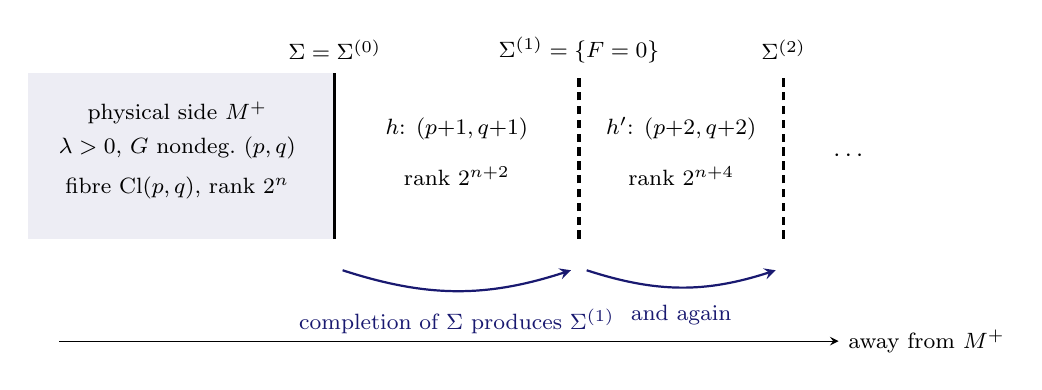
\begin{tikzpicture}[>=stealth, xscale=1.0,
  wall/.style={very thick},
  shadow/.style={very thick, densely dashed},
  lab/.style={font=\footnotesize, align=center}]
\fill[MidnightBlue!8] (-3.9,-1.05) rectangle (0,1.05);
\draw[wall] (0,-1.05) -- (0,1.05);
\draw[shadow] (3.1,-1.05) -- (3.1,1.05);
\draw[shadow] (5.7,-1.05) -- (5.7,1.05);
\node[font=\small] at (6.55,0) {$\cdots$};
\node[lab] at (0,1.35) {$\Sig = \Sig^{(0)}$};
\node[lab] at (3.1,1.35) {$\Sig^{(1)} = \{F = 0\}$};
\node[lab] at (5.7,1.35) {$\Sig^{(2)}$};
\node[lab] at (-2.0,0.55) {physical side $\Mp$};
\node[lab] at (-2.0,0.1) {$\lambda > 0$, $G$ nondeg.\ $(p,q)$};
\node[lab] at (-2.0,-0.4) {fibre $\Cl(p,q)$, rank $2^n$};
\node[lab] at (1.55,0.35) {$h$: $(p{+}1,q{+}1)$};
\node[lab] at (1.55,-0.25) {rank $2^{n+2}$};
\node[lab] at (4.4,0.35) {$h'$: $(p{+}2,q{+}2)$};
\node[lab] at (4.4,-0.25) {rank $2^{n+4}$};
\draw[->, thick, MidnightBlue] (0.1,-1.45) to[bend right=18] node[below, lab, yshift=-1mm] {completion of $\Sig$ produces $\Sig^{(1)}$} (3.0,-1.45);
\draw[->, thick, MidnightBlue] (3.2,-1.45) to[bend right=18] node[below, lab, yshift=-1mm] {and again} (5.6,-1.45);
\draw[->, thin] (-3.5,-2.35) -- (6.4,-2.35) node[right, lab] {away from $\Mp$};
\end{tikzpicture}
\caption{The wall sequence, displaced successively away from the physical region. The metric $G$ is nondegenerate of signature $(p,q)$ on the shaded physical side $\Mp$ and degenerates tamely on the wall $\Sig$. The one-sided completion $h$ (Theorem \ref{thm:onesided}) is nondegenerate of signature $(p{+}1,q{+}1)$ on all of $\Mp$, wall included, but by conservation of degeneracy (Theorem \ref{thm:absolute}) it cannot be nondegenerate on both sides: it degenerates on the displaced shadow wall $\Sig^{(1)}$, the zero set of the determinant factor $F$ (Proposition \ref{prop:conservation}), across which its signature passes to $(p,q{+}2)$. For good couplings $\Sig^{(1)}$ is itself tame (Lemma \ref{lem:wallinduction}), so the completion iterates: each wall's completion resolves it and produces the next, one Rule-1 rung $\Cl(p{+}k,q{+}k) \to \Cl(p{+}k{+}1,q{+}k{+}1)$ per wall, along an infinite sequence displaced ever further from the physical region (Corollary \ref{cor:wallsequence}). Degeneracy is moved, never destroyed.}
\label{fig:wallsequence}
\end{figure}

\begin{theorem}[Conservation of degeneracy, absolute form]\label{thm:absolute}
Let $M$ be connected, let $(M,G)$ be a tame corank-one degeneration whose two open sides $\Mp \setminus \Sig$ and $M \setminus \Mp$ are both nonempty, let $E \to M$ be \emph{any} vector bundle containing $T^*M$ as a subbundle, carrying \emph{any} smooth symmetric form $h$ which is \emph{standard} outside some neighbourhood $U$ of $\Sig$ with $M \setminus U$ meeting both sides: there, $h = G \perp K$ for a nondegenerate form $K$ on a complement, with $\operatorname{sig}(K)$ the same on both exterior regions. Then $h$ is not nondegenerate everywhere: every completion of a signature-change cometric that is standard, in this sense, outside a neighbourhood of the wall degenerates somewhere. Degeneracy can be displaced, never destroyed.
\end{theorem}

\begin{proof}
The signature of a continuous nondegenerate symmetric form on a connected base is constant: the eigenvalues of its Gram matrix with respect to any auxiliary frame metric vary continuously and never vanish, so their sign counts are locally constant, and $M$ is connected. Suppose $h$ nondegenerate everywhere. On the physical exterior $h = G \perp K$ has signature $(p,q) + \operatorname{sig}(K)$; on the far exterior it has $(p{-}1, q{+}1) + \operatorname{sig}(K)$ (Remark \ref{rem:coords}), with the \emph{same} $\operatorname{sig}(K)$ by the standardness hypothesis. The two totals differ in the first entry by one; a single form of constant signature cannot have both, so nondegeneracy must fail somewhere in $U$. The constancy clause on $\operatorname{sig}(K)$ is necessary: $M \setminus U$ is disconnected (the two sides lie in different components of $M \setminus \Sig$), and a completion allowed to switch $K$'s signature across the wall, say from $(1,1)$ to $(2,0)$, could match the two totals; ``standard'' means one exterior model, not two.
\end{proof}

\begin{proposition}[Conservation of degeneracy, located]\label{prop:conservation}
With the sign $\mu\nu > 0$ required for Theorem \ref{thm:onesided}, the ambient form $h$ of Definition \ref{def:coupling} degenerates exactly on the zero set of $F = 1 + 2\mu\nu\beta^2 s$ within $M \setminus \Sig$, and this zero set is nonempty on the far side of every transversal: a displaced degeneration locus $\Sig'$ (the \emph{shadow wall}) separating $\Sig$ from the far exterior. Between $\Sig$ and the shadow wall the ambient signature remains $(p{+}1, q{+}1)$; across any simple zero of $F$ it passes to $(p, q{+}2)$. Choosing $\mu\nu < 0$ instead exchanges the roles of the two sides: $h|_\Sig$ has signature $(p, q{+}2)$, which is the Rule-1 ascent of the far side's algebra $\Cl(p{-}1, q{+}1)$, and the degeneration is displaced into the physical side. No choice of coupling sign yields a two-sided completion of constant signature, as Theorem \ref{thm:absolute} independently guarantees.
\end{proposition}

\begin{proof}
Off $\Sig$ the form $G$ is invertible, so by Lemma \ref{lem:det}(1) $\det h = \det G \cdot (-F)$ vanishes exactly where $F$ does. Along a far-side transversal: near the wall $\beta = 1$ and $s \to -\infty$ (Lemma \ref{lem:det}(2), $\lambda < 0$ there), so $F \to -\infty$; outside the collar $\beta = 0$ and $F = 1$. By continuity $F$ vanishes at some intermediate point, and the set $\{F = 0\}$ separates the two regimes on every transversal. Signatures: on the far-side region between $\Sig$ and the first zero of $F$, $h$ is nondegenerate ($F < 0$ there, by continuity from $F \to -\infty$ and no intervening zero), and this region's closure meets $\Sig$, where the signature is $(p{+}1,q{+}1)$ by Lemma \ref{lem:wallgram}; local constancy propagates it. Across a simple zero of $F$ the determinant $\det h$ changes sign through a simple zero, so (with respect to an auxiliary frame metric) exactly one eigenvalue of $h$ crosses zero, to first order: were two or more to vanish at the crossing point, $\det h$ would vanish there to order at least two. Which way the crossing goes is decided by the Schur complement, not by the determinant alone (a crossing to $(p{+}2, q)$ would produce the same determinant sign): off $\Sig$ the block congruence of Lemma \ref{lem:det} gives $h \cong G \perp S$ with $S = H - \beta^2 s \begin{psmallmatrix} \nu^2 & \mu\nu \\ \mu\nu & \mu^2 \end{psmallmatrix}$, $\det S = -F$ and $\operatorname{tr} S = -\beta^2 s\,(\mu^2 + \nu^2)$. At a far-side zero of $F$ we have $2\mu\nu\beta^2 s = -1$ with $\mu\nu > 0$, so $s < 0$ and $\operatorname{tr} S > 0$: as $F$ crosses zero, $S$ passes from $\det S > 0$ with positive trace, signature $(2,0)$, to $\det S < 0$, signature $(1,1)$, while the $G$-block stays at $(p{-}1, q{+}1)$. The total therefore passes from $(p{+}1, q{+}1)$ to $(p, q{+}2)$: it is a \emph{positive} direction that degenerates. For $\mu\nu < 0$: Lemma \ref{lem:wallgram}(4) gives $(p, q{+}2)$ on the wall, which is $((p{-}1){+}1, (q{+}1){+}1)$, the ascent of the far side; and the argument above mirrors, with $s \to +\infty$ on the physical side making $F \to -\infty$ there. Finally $\mu\nu = 0$ is excluded by the wall Gram's determinant $-2\mu\nu$.
\end{proof}

\begin{lemma}[Tame wall induction]\label{lem:wallinduction}
Assume $\Sig$ compact, and fix the collar. Near the wall, on the far side, $s$ is strictly monotone along transversals: $s = 1/\lambda + O(1)$ with derivative $s' = -\lambda'/\lambda^2\,(1 + o(1)) \neq 0$, since the singular term dominates the bounded derivative of the smooth remainder; call the (relatively compact) region where this monotonicity holds the \emph{monotone zone}, and let
\[
S \;:=\; \sup\,|s| \quad\text{over the far-side part of the collar \emph{outside} the monotone zone}
\]
(finite: that region has compact closure avoiding $\Sig$). Call the coupling \emph{good} if $|\mu\nu| < 1/(2S)$. For good couplings:
\begin{enumerate}
\item every far-side zero of $F$ lies in the monotone zone with $\beta \equiv 1$ there, so the shadow wall $\Sig'$ is the regular level set $\{F = 0\}$ with $dF = 2\mu\nu\,ds \neq 0$ transversally: a smooth closed hypersurface, and the zero of $\det h$ across it is simple;
\item at each point of $\Sig'$ exactly one $h$-eigenvalue (with respect to an auxiliary frame metric) vanishes, to first order, and the radical line of $h|_{\Sig'}$ is a smooth line subbundle: it is the column space of the adjugate $\operatorname{adj}(h)$, which has rank one along $\Sig'$;
\item the invariant transversality datum of Lemma \ref{lem:invariantT2} (which makes sense verbatim for any bundle with symmetric form) is nowhere zero on $\Sig'$: by Jacobi's formula the simplicity of the zero of $\det h$ \emph{is} the transversality of the degeneration.
\end{enumerate}
Hence $(T, h)$ is itself a tame corank-one degeneration along $\Sig'$, in the bundle-valued sense of Remark \ref{rem:bundlesetup}. The completion therefore iterates: each wall's ambient form is a tame degeneration with its own shadow wall, and the infinite wall sequence exists unconditionally for good couplings, not merely generically.
\end{lemma}

\begin{proof}
\emph{The monotone zone, and finiteness of $S$.} By Lemma \ref{lem:det}(2), $s = 1/\lambda + b$ with $b$ smooth up to the wall, locally uniformly; so $s' = -\lambda'/\lambda^2 + b'$, and since $\lambda \to 0$ while $\lambda'$ is bounded away from zero near $\Sig$ (T3) and $b'$ is bounded (compactness of $\Sig$ makes all these bounds uniform along the wall), there is a one-sided collar neighbourhood on which $|\lambda'|/\lambda^2 > |b'|$: the monotone zone. Its far-side complement within the collar has compact closure disjoint from $\Sig$, on which the smooth function $s$ is bounded: $S < \infty$.

(1) Outside the collar $F = 1$; on the far collar side outside the monotone zone, $|2\mu\nu\beta^2 s| \leq 2|\mu\nu| S < 1$, so $F > 0$: no zeros in either region, whatever $\beta$ does there. All far-side zeros therefore lie in the monotone zone. Approaching the wall $F \to -\infty$ (Lemma \ref{lem:det}(2)) and at the zone's outer edge $F > 0$, so each transversal carries a zero; where $\beta \equiv 1$ (shrink the zone into the inner collar if necessary), $F = 1 + 2\mu\nu s$ is strictly monotone along each transversal with a single simple zero, and $dF = 2\mu\nu\, ds$ has nonvanishing transversal component $2\mu\nu s' \neq 0$: $\{F = 0\}$ is a regular level set, a smooth closed hypersurface $\Sig'$, and $\det h = \det G \cdot (-F)$ has a simple zero across it ($\det G \neq 0$ there).

(2) At a simple zero of $\det h = \prod_i \mu_i$ (eigenvalues with respect to the auxiliary metric), exactly one eigenvalue $\mu_1$ vanishes and to first order: two vanishing eigenvalues would force a second-order zero. For the smoothness of the radical line, no spectral theory is needed: the adjugate $\operatorname{adj}(h)$, polynomial in the entries of $h$, is smooth; at a point of corank one it has rank exactly one (some $(d{-}1)$-minor is nonzero, and $h \cdot \operatorname{adj}(h) = \det(h)\,1 = 0$ puts every column of $\operatorname{adj}(h)$ in $\ker h$, which is a line). A nonvanishing column of $\operatorname{adj}(h)$ is therefore a smooth local spanning section of the radical line along $\Sig'$.

(3) Jacobi's formula, $\partial_\tau \det h = \operatorname{tr}\bigl(\operatorname{adj}(h)\, \partial_\tau h\bigr)$ (differentiate the determinant column by column and expand each along its differentiated column), evaluated at a point of $\Sig'$: in an auxiliary-orthonormal eigenbasis there, $\operatorname{adj}(h) = \bigl(\prod_{i \geq 2} \mu_i\bigr)\, \tilde k\, \tilde k^{\mathsf T}$ with $\tilde k$ the unit kernel vector, so
\[
\partial_\tau \det h \;=\; \Bigl(\prod_{i \geq 2} \mu_i\Bigr)\, (\partial_\tau h)(\tilde k, \tilde k) .
\]
The left side is nonzero (the zero of $\det h$ is simple, by (1)) and the nonvanishing eigenvalues $\mu_i$, $i \geq 2$, are nonzero; hence $(\partial_\tau h)(\tilde k, \tilde k) \neq 0$. This is exactly the nonvanishing of the datum $\delta'$ of Lemma \ref{lem:invariantT2} for $(T, h)$ along $\Sig'$: for any extension of $\tilde k$, $d\,h(\tilde k, \tilde k)|_{\Sig'} = (\partial_\tau h)(\tilde k, \tilde k)\, d\tau$, the cross term vanishing because $\tilde k$ is radical on $\Sig'$, and the lemma's proof uses only the symmetric form and the radical, not the cotangent origin of the bundle. So (T3) holds, (T1) and (T2) being parts (1) and (2).
\end{proof}

\begin{remark}[The setup generalises to arbitrary bundles]\label{rem:bundlesetup}
Sections \ref{sec:setup} and \ref{sec:degeneration}, and the completion of Section \ref{sec:ambient}, use nothing about $T^*M$ beyond its being a vector bundle with a smooth symmetric form: Hypotheses \ref{hyp:tame}, Lemma \ref{lem:invariantT2}, the blade basis, the degeneration sheaf and the coupling construction all apply verbatim to a pair $(E, h)$ with $E$ any real vector bundle of rank $m$, producing Clifford sheaves of rank $2^m$ and one-sided completions of rank $2^{m+2}$. Lemma \ref{lem:wallinduction} needs exactly this generality: the first iteration supplies the induction with the ambient pair $(T, h)$, of rank $n+2$, rather than a cometric.
\end{remark}

\begin{corollary}[The infinite wall sequence]\label{cor:wallsequence}
Let $\Sig$ be compact. For good couplings at every stage, there is an infinite sequence $\Sig = \Sig^{(0)}, \Sig^{(1)} = \Sig', \Sig^{(2)}, \dots$ of tame walls, each displaced from the last into the unphysical region, carrying Clifford sheaves of ranks $2^n, 2^{n+2}, 2^{n+4}, \dots$ whose physical-side fibres ascend the Witt tower $\Cl(p,q) \to \Cl(p{+}1,q{+}1) \to \Cl(p{+}2,q{+}2) \to \cdots$, one Rule-1 rung per wall. Degeneracy is conserved along the entire sequence: each completion resolves its wall and produces the next, displaced successively further from the physical region.
\end{corollary}

\begin{proof}
Induction on Lemma \ref{lem:wallinduction} via Remark \ref{rem:bundlesetup}, choosing at each stage a good coupling (possible: each $\Sig^{(k)}$ is a closed subset of a compact collar of its predecessor, hence compact, so its $S$ is finite, and only an upper bound on $|\mu\nu|$ is demanded). Each stage also needs its radical line trivial, so that collar data exist for the next coupling (Definition \ref{def:coupling}); this is automatic, because the shadow wall's radical line carries an explicit global spanning section: writing $\alpha_0 := G^{-1}e$ for the metric dual of the transversal functional, so that $s = \alpha_0(u)$, the section
\[
x \;:=\; \alpha_0 \,+\, \mu\beta s\, \nO \,+\, \nu\beta s\, \nInf
\]
satisfies $h(x, \alpha) = e(\alpha)\,(1 + 2\mu\nu\beta^2 s) = e(\alpha)\,F = 0$ on $\{F = 0\}$ for every $\alpha \in T^*M$, while $h(x, \nO) = \nu\beta s - \nu\beta s = 0$ and $h(x, \nInf) = \mu\beta s - \mu\beta s = 0$: so $x$ spans $\ker h$ along $\Sig'$, globally and without zeros. A global transversal for the next stage is then any $u'$ with $x(u') = 1$, available from any bundle metric. The ranks and signatures are Theorem \ref{thm:onesided} at each stage. Figure \ref{fig:wallsequence} displays the sequence.
\end{proof}

\begin{remark}[The wall class, posed]\label{rem:wallclass}
Degeneracy is conserved: it can be pushed off the physical region, never annihilated globally. This is the first geometric instance of the conservation principle conjectured at the fibre level in \cite[Conj.~7.9]{ButlerT1} (obstructions are moved, never destroyed), and the sharpest open question this paper poses is its measure: to construct a cohomological invariant on $\Sig$, presumably a relative class built from the mod-8 residues of the two competing ascents on the two sides of the wall, whose nonvanishing forces the shadow wall's existence, and whose behaviour under the iteration of Lemma \ref{lem:wallinduction} advances the clock of \cite[\S7]{ButlerT1}. The precise formulation is given in Section \ref{sec:dictionary} among the successor problems.
\end{remark}

\section{The exceptional algebra and the metric's residue}\label{sec:exceptional}

\begin{proposition}[The exceptional algebra: deformation to the normal cone]\label{prop:exceptional}
Fix $x \in \Sig$ and a transversal curve through $x$ with parameter $t$, so that $G(t) = G_0 + t\dot G + O(t^2)$ with radical of $G_0$ spanned by $k$ and $\dot G(k,k) \neq 0$ by (T3). Rescale anisotropically: fix a complement $V_1$ of the radical and send $k \mapsto k/\sqrt{t}$. Then the rescaled forms converge as $t \to 0^+$ to the nondegenerate form $\hat G := G_0|_{V_1} \perp \dot G(k,k)$ on $V_1 \oplus \R k$: the cross terms are suppressed by $\sqrt{t}$, and the dying direction re-enters with its rate of degeneration as its metric coefficient. On the physical side the limit has signature $(p, q)$. The rescaled Clifford family is therefore a continuous family of nondegenerate algebras through $t = 0$, and its special fibre $\shE(x) := \Cl(V_1 \oplus \R k, \hat G)$, the \emph{exceptional algebra} at $x$, is independent of the choice of complement and of the scales of $k$ and $t$ up to canonical isomorphism.
\end{proposition}

\begin{proof}
Compute the Gram matrix of the rescaled frame $(v_1, \dots, v_{n-1}, k/\sqrt{t})$, $v_i$ a basis of $V_1$, against $G(t)$:
\[
G(t)(v_i, v_j) = G_0(v_i,v_j) + t\dot G(v_i,v_j) + O(t^2) \;\longrightarrow\; G_0(v_i,v_j) ;
\]
\[
G(t)(v_i, k/\sqrt{t}) = \frac{G_0(v_i,k) + t\dot G(v_i,k) + O(t^2)}{\sqrt{t}} = \frac{0 + O(t)}{\sqrt{t}} = O(\sqrt{t}) \;\longrightarrow\; 0 ,
\]
using $G_0(v_i, k) = 0$ ($k$ is radical for $G_0$);
\[
G(t)(k/\sqrt{t},\, k/\sqrt{t}) = \frac{G_0(k,k) + t\dot G(k,k) + O(t^2)}{t} = \dot G(k,k) + O(t) \;\longrightarrow\; \dot G(k,k) \neq 0 .
\]
The limit Gram is block-diagonal: $G_0|_{V_1}$, nondegenerate of signature $(p{-}1,q)$ (Theorem \ref{thm:degsheaf}(2), via $V_1 \cong T^*_xM/\shL$), plus the $1 \times 1$ block $\dot G(k,k)$, positive on the physical side (Remark \ref{rem:coords}); so $\hat G$ is nondegenerate of signature $(p,q)$ there. All rescaled Gram entries are continuous functions of $\sqrt{t}$ on $[0, \varepsilon)$, and by Lemma \ref{lem:blades} the structure constants of the corresponding Clifford algebras are polynomial in them: the rescaled Clifford family is continuous through $t = 0$, with nondegenerate special fibre $\shE(x)$.

Independence. Changing the complement, $v \mapsto v + c(v)k$: the $V_1$-block entries change by $c(v)G_0(k, w) + c(w)G_0(v,k) + c(v)c(w)G_0(k,k) + O(t) = O(t)$, and the cross terms remain $O(\sqrt t)$, so the limit is unchanged, and the two limit forms are literally equal under the isomorphism $v + \R k \mapsto v' + \R k$ of $V_1 \oplus \R k$ with $V_1' \oplus \R k$ fixing $k$ and matching complements through the quotient $T^*_xM/\shL$. Rescaling $k \mapsto ck$ multiplies the diagonal limit entry by $c^2$ and the generator by $c$: the map $v_i \mapsto v_i$, $k \mapsto ck$ is an isometry of the two limit forms, inducing a canonical isomorphism of the Clifford algebras. Reparametrising $t \mapsto at$ ($a > 0$) multiplies $\dot G$ by $a$ and the rescaled generator $k/\sqrt{t}$ by $1/\sqrt{a}$; the two effects compose to the isometry $k \mapsto k/\sqrt a$ against the $a$-fold entry, again canonical. In each case the displayed isometry is built from the change of data alone, with no further choices, and the isomorphism of Clifford algebras it induces by functoriality is the canonical identification meant in the statement. (Uniqueness among all isometries fixing the $V_1$-part fails, $k \mapsto -k$ being another; canonicality here means choice-freeness of the displayed maps, not uniqueness.)
\end{proof}

\begin{theorem}[The metric's residue, and the square-root twist]\label{thm:residue}
At a tame wall the physical metric (the inverse cometric) has a canonical simple pole: for any defining function $\tau$ of $\Sig$,
\[
O \;:=\; \lim_{\tau \to 0}\, \tau\, G^{-1} \;=\; \frac{k \otimes k}{\delta(k \otimes k)/d\tau} ,
\]
a nowhere-vanishing section of $\shL \otimes \shL$ depending on $\tau$ through the weight of a section of $\shL \otimes \shL \otimes N\Sig$; invariantly, the residue is $\delta^{-1}$, the inverse of the transversality datum of Lemma \ref{lem:invariantT2}, regarded as a section of $\shL \otimes \shL \otimes N\Sig = \operatorname{Hom}(N^*\Sig, \shL^{\otimes 2})$. It is a nondegenerate pairing between $\shL^* \otimes \shL^*$ and $N^*\Sig$, hence induces a canonical isomorphism
\[
N^*\Sig \;\cong\; \shL^{\otimes 2} :
\]
the conormal bundle is the square of the dying direction itself. Dually, $N\Sig \cong (\shL^*)^{\otimes 2}$: the Witt partner line adjoined by the completion, which the pairing normalisation $kk^* + k^*k = 1$ identifies with $\shL^*$, is a canonical square root of the \emph{normal} bundle, and the dying line $\shL$ is a canonical square root of the conormal bundle. (The reading of the blow-up rescaling $k \mapsto k/\sqrt{t}$ as the normalisation of a conormal square root is Remark \ref{rem:blowup}.)
\end{theorem}

\begin{proof}
Work in the frame $(k, m_1, \dots, m_{n-1})$ of Remark \ref{rem:coords} along a transversal with parameter $\tau$, with Gram $G(\tau) = \begin{psmallmatrix} \lambda & b^{\mathsf T} \\ b & G_1 \end{psmallmatrix}$, $\lambda(0) = 0$, $b(0) = 0$, $G_1(0)$ invertible, and $\lambda'(0) =: T \neq 0$, so that $\delta(k \otimes k) = T\, d\tau$. The inverse cometric $G^{-1}$, a symmetric form on $TM$, has matrix $C := [\text{Gram}]^{-1}$ with respect to the covector basis, meaning $G^{-1} = \sum C_{ab}\, \kappa_a \otimes \kappa_b$ over the frame covectors $\kappa = (k, m)$. Block inversion:
\[
C_{00} = (\lambda - b^{\mathsf T} G_1^{-1} b)^{-1} = \frac{1}{T\tau}\bigl(1 + O(\tau)\bigr), \qquad
C_{0i} = -C_{00}\, (b^{\mathsf T} G_1^{-1})_i = O(1),
\]
since $b = O(\tau)$ makes $b^{\mathsf T} G_1^{-1} b = O(\tau^2)$ and $C_{00}\,O(\tau) = O(1)$; and the $m$-block of $C$ is $G_1^{-1} + G_1^{-1} b\, C_{00}\, b^{\mathsf T} G_1^{-1} = O(1)$. Multiplying by $\tau$ and letting $\tau \to 0$, every entry goes to zero except the top-left:
\[
\tau\, G^{-1} \;\longrightarrow\; \frac{1}{T}\, k \otimes k .
\]
Independence of the extension of $k$: by Lemma \ref{lem:invariantT2}(2) the derivative $T = dg_k(\partial_\tau)|_\Sig$ is extension-independent. Dependence on the scale of $k$: $k \mapsto ck$ multiplies the numerator $k \otimes k$ by $c^2$ and $T$ by $c^2$ (Lemma \ref{lem:invariantT2}(3)); the limit is unchanged, so the residue does not depend on $k$ at all, only on the line $\shL$ and the degeneration. Dependence on $\tau$: replacing $\tau$ by $a\tau$ ($a > 0$ smooth) multiplies the limit by $a|_\Sig$, exactly the transformation of the $d\tau$-coefficient of a section of $N\Sig$; the assignment $d\tau \mapsto \lim \tau G^{-1}$ is therefore a well-defined homomorphism $N^*\Sig \to \shL^{\otimes 2}$, and the computation identifies it as $d\tau \mapsto (1/T)\,k \otimes k = \delta^{-1}(d\tau)$: the analytic residue \emph{is} the algebraic transversality datum, inverted. It is nowhere vanishing because $\delta$ is an isomorphism under (T3). A nowhere-vanishing homomorphism between line bundles is an isomorphism, giving $N^*\Sig \cong \shL^{\otimes 2}$ (equivalently, the nondegenerate pairing $(\shL^* \otimes \shL^*) \otimes N^*\Sig \to \R$ induced by $\delta^{-1}$, whence $N^*\Sig \cong (\shL^* \otimes \shL^*)^* = \shL^{\otimes 2}$); dualising gives $N\Sig \cong (\shL^*)^{\otimes 2}$. The partner identification: in the ambient completion, $k^* = \nO/(2\nu)$ satisfies $kk^* + k^*k = 1$ (Corollary \ref{cor:localised}), so rescaling $k \mapsto ck$ forces $k^* \mapsto k^*/c$: the partner line is canonically $\shL^*$, hence a square root of $N\Sig$. Finally, $\shL^{\otimes 2} \cong N^*\Sig$ says exactly that $k$ carries the weight of a half-power of a defining function, and $k/\sqrt t$ is weightless: the rescaling of Proposition \ref{prop:exceptional} is the canonical normalisation.
\end{proof}

\begin{remark}[The direction of the induced twist]\label{rem:twistcorrection}
The pairing argument fixes which way the isomorphism runs, and the direction is easy to state the wrong way round, so it is worth recording. A nondegenerate pairing between $\shL^* \otimes \shL^*$ and $N^*\Sig$ identifies $N^*\Sig$ with $(\shL^* \otimes \shL^*)^* = \shL^{\otimes 2}$, and not with $(\shL^*)^{\otimes 2}$. The identifications, proved above and forced already by Lemma \ref{lem:invariantT2} (where $\delta : \shL^{\otimes 2} \to N^*\Sig$ lands in the conormal bundle by construction), are therefore: the \emph{dying line} squares to the conormal bundle, and the \emph{partner line} squares to the normal bundle. Everything downstream is stated in that form: the half-power rescaling $k \mapsto k/\sqrt t$, the weightlessness of the normalisation $kk^* + k^*k = 1$ (the two half-weights cancel), and the square-root form of the residue identity.
\end{remark}

\begin{remark}[Blow-up dictionary]\label{rem:blowup}
Proposition \ref{prop:exceptional} is the deformation to the normal cone \cite[Ch.~5]{Fulton1998} transcribed into Clifford algebra: the exceptional algebra over $x \in \Sig$ is built from the surviving tangential form together with the normal derivative of the degeneration, normal-cone data alone, exactly as the exceptional divisor of a blow-up replaces each point of the centre by its normal directions. The substitution $k \mapsto k/\sqrt{t}$ is the blow-up chart; the ambient description of Section \ref{sec:ambient} and the rescaled description here are its two standard charts; and Theorem \ref{thm:residue} identifies the tautological bundle of the correspondence: not $\shL^* \otimes N^*\Sig$ but the square-root identity. Since $\shL^{\otimes 2} \cong N^*\Sig$ says that $k$ carries the weight of a half-power of a defining function, the rescaling is exactly the normalisation of a conormal square root by the inverse square root of the defining function: the adjoined dimension is constructed tautologically from the dying direction and the geometry of its degeneration.
\end{remark}

\section{Dictionary, choices, and scope}\label{sec:dictionary}

This section is deliberately two-tier. The topological consequences of the residue theorem, and the itemisation of the construction's global choices, are proved at the standard of the rest of the paper. The dictionary with tractor calculus and the ambient metric is \emph{assembly}: a precise correspondence of structures, stated carefully, without the claim that either construction is a special case of the other. The scope declarations at the end delimit what this paper's methods reach.

\subsection{Topology of tame walls, and the global choices}\label{subsec:choices}

\begin{corollary}[Tame walls are two-sided]\label{cor:twosided}
For any tame corank-one degeneration, the conormal bundle of $\Sig$ satisfies $N^*\Sig \cong \shL^{\otimes 2}$ (Theorem \ref{thm:residue}), hence has vanishing first Stiefel-Whitney class: $w_1(N^*\Sig) = 2\,w_1(\shL) = 0$. So $N\Sig$ is trivial, $\Sig$ is two-sided in $M$, and a global side choice (a co-orientation, hence the meaning of ``the physical side'') always exists. Tameness itself forbids one-sided walls: a hypersurface with M\"obius normal bundle admits no corank-one degeneration satisfying (T1)-(T3) along it.
\end{corollary}

\begin{proof}
A square of a real line bundle has trivial $w_1$ and a real line bundle is trivial exactly when its $w_1$ vanishes (Fact \ref{fact:linebundles}); an isomorphism preserves $w_1$, and $N\Sig \cong (N^*\Sig)^*$ shares triviality. Two-sidedness of a hypersurface is triviality of its normal bundle (Fact \ref{fact:linebundles}).
\end{proof}

The construction's global inputs, and what obstructs them, are then exactly these:

\begin{enumerate}
\item \textbf{The side.} Always available, by Corollary \ref{cor:twosided}; the residual choice is a global sign, a torsor over $H^0(\Sig; \mathbb{Z}_2)$, fixed in the gravitational application by physics (the Lorentzian side).
\item \textbf{Orientation of the radical line.} The spanning section $k$ exists globally iff $\shL$ is trivial, iff $w_1(\shL) = 0 \in H^1(\Sig; \mathbb{Z}_2)$ (Fact \ref{fact:linebundles}). The constructions divide over this class. The ideal sheaf and the residue are quadratic or scale-covariant in $k$, so they descend to the line bundle and need nothing. The \emph{coupling} does not descend: it is of weight $-1$ in $k$ (the transversal $u$ with $k(u) = 1$ is itself a trivialisation of $\shL^*$), so collar data, and with them the completion of Theorem \ref{thm:onesided} in the untwisted plane $\underline{\R}^2$, exist exactly when $w_1(\shL) = 0$, which is why Definition \ref{def:coupling} carries that standing hypothesis. For $w_1(\shL) \neq 0$, which is possible and marks walls whose dying direction is globally non-orientable, the residue theorem's conclusion that the partner line is canonically $\shL^*$ dictates the repair: the adjoined plane must be the $\shL$-twisted plane $\shL \oplus \shL^*$ rather than $\underline{\R}^2$. That twisted variant is not developed here and is recorded among the successor problems. The class $w_1(\shL)$ is a genuine invariant of the degeneration, constrained by the residue theorem to satisfy $2 w_1(\shL) = w_1(N^*\Sig) = 0$, which is no constraint mod 2.
\item \textbf{The transversal field and the collar.} Given the global $k$ of item 2, the space of pairs $(u, \beta)$ with $k(u) = 1$ is convex, hence contractible: no further obstruction, and any two choices are homotopic through admissible choices.
\item \textbf{The coupling constants.} Only the product $\mu\nu$ enters (Remark \ref{rem:signchoice}); the good-coupling condition of Lemma \ref{lem:wallinduction} is an open condition $0 < |\mu\nu| < 1/(2S)$, contractible at each fixed sign of $\mu\nu$ (as a condition on the product; the set of pairs $(\mu,\nu)$ has one contractible component per sign choice of each factor). The discrete datum is the sign of $\mu\nu$, i.e.\ which side's ascent is performed: combined with item 1 this is the only genuinely binary global choice, and the two options are exchanged by relabelling the sides.
\end{enumerate}

\subsection{The wall class, posed precisely}\label{subsec:wallclass}

Write $d := p - q \bmod 8$ for the clock position of the physical side's fibre algebra \cite[\S7]{ButlerT1}. Across $\Sig$ the metric signature passes to $(p{-}1, q{+}1)$, of clock position $d - 2$; the completion ascends both by $(+1,+1)$, which fixes clock position; and each iteration of Lemma \ref{lem:wallinduction} produces a new wall again separating clock positions differing by $2$. The data of a tame wall thus includes the locally constant function
\[
w(\Sig) \;:=\; \bigl(d,\, d-2\bigr) \in H^0\bigl(\Sig;\, \mathbb{Z}_8 \times \mathbb{Z}_8\bigr),
\]
the ordered pair of clock positions of the two competing ascents.

\begin{conjecture}[The wall class]\label{conj:wallclass}
There is a natural invariant of tame walls, built from $w(\Sig)$ and the torsion of the pair $(\shL, N^*\Sig)$, with the properties: (a) it vanishes iff some completion standard outside a collar is nondegenerate on \emph{both} sides (by Theorem \ref{thm:absolute}, it must therefore be nonvanishing whenever both sides are nonempty and the clock positions differ); (b) it is conserved under the wall induction of Lemma \ref{lem:wallinduction}, each iteration transferring it to the next shadow wall while shifting both clock coordinates by the rung; (c) it refines, at sheaf level, the conservation-of-obstruction conjecture of \cite[Conj.~7.9]{ButlerT1}, whose fibre-level content is the mod-8 obstruction of the transport rules. Theorem \ref{thm:absolute} proves the existence half of (a) in signature terms; the conjecture is that the signature mismatch is the coarse part of a finer, torsion-sensitive class whose vanishing is also sufficient.
\end{conjecture}

The evidence: the absolute conservation theorem shows the invariant's coarse part (the signature difference, equivalently the clock mismatch $2 \in \mathbb{Z}_8$) already obstructs; what remains open is whether the finer data ($w_1(\shL)$, the co-orientation, the mod-8 lift) obstruct independently, and whether (b) holds in the strong transfer form. This is successor material for the series' geometric papers.

\subsection{Dictionary: tractors and the ambient metric}\label{subsec:tractordict}

The following correspondences are assembly-level: precise at the level of the structures named, with the differences stated, and with no claim of subsumption either way.

\emph{Tractor calculus} \cite{BEG1994, CurryGover2018} attaches to an $n$-dimensional conformal manifold of signature $(p,q)$ the standard tractor bundle $\mathcal{T}$, of rank $n + 2$ and signature $(p{+}1, q{+}1)$, with a composition series whose successive quotients are the density bundles $\Lambda^0[1]$, $T^*M[1]$, $\Lambda^0[-1]$, and a canonical (normal) tractor connection. The correspondences: the ambient bundle $T = T^*M \oplus \underline{\R}^2$ matches the underlying filtered bundle, with $\nO, \nInf$ the two weight lines (the ``point at zero'' and ``point at infinity'' slots of the conformal sphere model); the ambient form $h$ matches the tractor metric; the completion's increment $(p,q) \to (p{+}1,q{+}1)$ is the tractor increment. The differences: tractor calculus starts from a \emph{conformal class} on all of $M$ and its bundle carries a canonical connection; the present construction starts from a single \emph{degenerating} cometric, carries no distinguished connection (none is needed for the algebra), and its coupling is supported near the wall, where conformal rescaling is precisely what fails. The natural meeting point, flagged as a question rather than claimed: at a conformally regularised wall (the CCC picture \cite{Penrose2010}), the conformal class extends across $\Sig$ while the metric degenerates, and there the ambient sheaf should be canonically the tractor bundle of the extended class, with the coupling the almost-Einstein scale tractor; making that precise is successor work.

\emph{The Fefferman-Graham ambient metric} \cite{FG1985, FG2012} realises the same $(+1,+1)$ increment as a nondegenerate metric of signature $(p{+}1,q{+}1)$ on a thickening $\widetilde{M} \subset \R_+ \times M \times \R$ of the metric cone. The correspondence: the FG cone directions (the dilation and the transversal) match the hyperbolic plane $(\nO, \nInf)$; the FG normalisation (Ricci-flatness to infinite or determined order) plays the role that the coupling's collar normalisation plays here. The difference is categorical: FG produces a manifold with metric, this paper produces a bundle with form; the Clifford functor applied to the FG tangent bundle along the cone's zero section reproduces the fibres of the ambient sheaf, but the sheaf exists without any thickened manifold, which is what permits the degenerate locus to be handled at all.

\subsection{Scope, and successor problems}\label{subsec:scope}

The tame class (T1)-(T3) is the boundary of Sections \ref{sec:setup} through \ref{sec:exceptional}, and each failure mode is either executed in Section \ref{sec:schwarzschild} or assigned to a named successor. \textbf{Anisotropic degeneration}: when different directions degenerate at different rates, the single rescaling $k \mapsto k/\sqrt t$ must be replaced by direction-dependent weights; the conjecture that the correct weights are the Kasner exponents of the BKL limit, and that the exceptional algebra of a black-hole singularity is the Clifford algebra of its Kasner form, is the \emph{Kasner-weights conjecture} of this programme. Section \ref{sec:schwarzschild} settles it for exact Schwarzschild in the diagonal class, where the weights are forced (Theorem \ref{thm:weights}), and Section \ref{sec:anisotropic} closes the diagonal class with position-dependent exponents at the algebraic level, stably under relatively admissible errors; what remains is the analytic dictionary with the admissibility class of \cite{ButlerT6}. \textbf{Higher codimension}: the Schwarzschild worldline has codimension three; hypersurface methods apply only after a geometric blow-up replacing the worldline by its normal sphere bundle. Section \ref{sec:schwarzschild} carries out the composite (geometric blow-up, then tame completion on the exceptional boundary) for exact Schwarzschild. For Kerr, whose ring has codimension two, the degeneration is of a genuinely new kind: preliminary computation by the methods of Section \ref{sec:schwarzschild} indicates that on the oblate blow-up the mass divergence concentrates as a rank-one null pulse along the lightlike ring generator, winding as the normal-circle cosine and vanishing on the two disc directions, so that fixed-power weights fail, the variable-order methods of Section \ref{sec:anisotropic} together with a focal double cover appears forced, and the winding-three duality monodromy conjectured in \cite{ButlerT6} appears as an integer winding on the oblate exceptional circle; the Kerr composite itself remains open. \textbf{Edge regularity}: where a tame wall meets a boundary or corner, the collar constructions need uniform control not provided here. \textbf{The twisted completion}: for walls with non-orientable dying direction, $w_1(\shL) \neq 0$, the coupling construction requires the $\shL$-twisted ambient plane $\shL \oplus \shL^*$ in place of $\underline{\R}^2$ (Section \ref{subsec:choices}, item 2); the twisted variant of Theorem \ref{thm:onesided} is expected to be routine but is not carried out here. \textbf{The wall class}: Conjecture \ref{conj:wallclass}. Within the tame class, nothing is left conditional: every statement of Sections \ref{sec:degeneration} through \ref{sec:exceptional} is proved, the boundary extension of Section \ref{sec:schwarzschild} is proved for exact Schwarzschild, and the variable-weight extension of Section \ref{sec:anisotropic} is proved for the relatively admissible diagonal class.

\section{The Schwarzschild composite}\label{sec:schwarzschild}

The tame class stops short of the black hole on two separate counts, both recorded in Remark \ref{rem:tamescope}: the Schwarzschild singularity is a worldline, of codimension three, and its degeneration is anisotropic, different directions degenerating at different rates. Section \ref{subsec:scope} names the repairs: a geometric blow-up replacing the worldline by its normal sphere bundle, and direction-dependent weights in place of the single $\sqrt t$ rescaling, with the Kasner-weights conjecture that the correct weights are the Kasner exponents. This section executes the composite for exact Schwarzschild.

The finding that makes it tractable is that the two gaps are not independent obstacles to be cleared one after the other. The blow-up closes most of the anisotropy by itself: the two angular rates are exactly the tautological rescaling that the exceptional divisor of any blow-up carries (the normal sphere at parameter $r$ has radius $r$), so after the blow-up only \emph{one} direction still degenerates, and it does so at first order in the defining function. Anisotropy at codimension three, restricted to this case, is codimension-one tameness expressed in polar coordinates.

Three costs are incurred, and they are stated here. First, the wall is now a \emph{boundary} of the blown-up manifold rather than an interior hypersurface, so the tameness hypotheses need one-sided restatements; these turn out to make the completion easier, not harder, and to make the conservation theorem vacuous in a way that is itself instructive. Second, the corank-one structure lies on a \emph{weighted} coframe module $\shW$ rather than on the cotangent bundle; the module is not a choice, being characterised as the bounded-norm one-forms of the quasihomogeneous blow-up, and the weights it encodes are unique and are the Kasner exponents. Third, everything here is exact Schwarzschild; the general anisotropic class, and Kerr, remain open and are itemised at the end.

Two inputs are imported from outside this paper, per the series' import discipline.

\begin{fact}[The gauge field and its cometric]\label{fact:pg}
In gauge theory gravity the Schwarzschild solution in the Newtonian (Painlev\'e-Gullstrand) gauge is carried by $\hb = 1 - \beta P$, $\beta = \sqrt{2M/r}$, $P(a) = (a \cdot e_t)\,e_r$, with $P^2 = 0$; $\hb$ is invertible in closed form at every $r > 0$, horizon included, and fails at $r = 0$ through a null kernel. The induced metric is the Painlev\'e-Gullstrand line element $ds^2 = dt^2 - (dr + \beta\,dt)^2 - r^2 d\Omega^2$. \emph{Provenance:} \cite{ButlerT5}, Props.~2.2, 2.4, 2.5 and 2.6, and Appendix A; the gauge-theoretic background is \cite{DoranLasenby2003}.
\end{fact}

\begin{fact}[Kasner data of the interior]\label{fact:kasner}
Along the approach to the Schwarzschild singularity the metric takes Kasner form \cite{Kasner1921} with exponents $(p_1, p_2, p_3) = (-\tfrac13, \tfrac23, \tfrac23)$, $\sum p_i = \sum p_i^2 = 1$, in proper time $\tau_{\mathrm{p}} \propto r^{3/2}$. \emph{Provenance:} classical; proved exactly, with rates, in the Kasner form lemma of \cite{ButlerT6}.
\end{fact}

\noindent\textbf{Conventions.} Units $G = c = 1$; to keep the arithmetic exact we write $2M = m^2$ and work in the variable $u := \sqrt{r}$, so that $\beta = m/u$ is rational in $u$. The defining function of the singular boundary is $r = u^2$; ``first order in $r$'' reads ``second order in $u$''. Signature convention $({+},{-},{-},{-})$. Throughout this section $E$ denotes the singular boundary (not the auxiliary bundle of Theorem \ref{thm:absolute}); the coupling constants $\mu, \nu$ of Definition \ref{def:coupling} always appear as the product $\mu\nu$, while the angular coframe elements are the subscripted $\mu_1, \mu_2$. One conormal convention, used throughout: on $\Mt_u$ the smooth defining function of $E$ is $u$, and $dr = 2u\,du$ vanishes on $E$ as a $u$-smooth one-form; the boundary data of the tame theory are graded by $r$, so the conormal line in which the transversality datum and the residue lie is the $r$-conormal $N^*_r E := (N^*_u E)^{\otimes 2}$, spanned by the class of $dr$, matching the first-order-in-$r$ clause of (T3$\partial$).

\subsection{The blow-up and the weighted module}\label{subsec:schwblowup}

On the flat background of Fact \ref{fact:pg} the singular locus of $\hb$ is the worldline $\ell = \{r = 0\}$, of codimension three. Let $\Mt$ denote the real oriented blow-up of the background along $\ell$: concretely, $\Mt = \R_t \times [0,\infty)_r \times S^2$, with boundary
\[
E \;=\; \{r = 0\} \;\cong\; \R \times S^2 ,
\]
which is a \emph{hypersurface}: codimension one in $\Mt$. Polar coordinates realise the blow-up; nothing more sophisticated is needed. Each point of the worldline has been replaced by the sphere of normal directions, exactly as Section \ref{subsec:scope} prescribes.

On $\Mt$ the cometric does not extend to $E$ in the coordinate coframe: some components vanish and others diverge, at different rates, which is the anisotropy problem restated. The resolution is to change not the geometry but the \emph{module of coframes} in which the geometry is expressed. The construction, a rescaled bundle at a boundary, is standard in boundary index theory \cite{Melrose1993}; what is particular here is that the metric itself characterises the rescaling.

\begin{definition}[The weighted coframe module]\label{def:W}
Let $\Mt_u$ denote $\Mt$ with the quasihomogeneous smooth structure of order two at the boundary: smooth functions of $(u, t, \omega)$, $u = \sqrt{r}$. Define $\shW$ as the $C^\infty(\Mt_u)$-module with frame
\[
\rho := r^{1/2}\,dr \;(= 2u^2\,du), \qquad \dtPG, \qquad \mu_1 := r\,d\theta, \qquad \mu_2 := r\sin\theta\,d\phi ,
\]
where $t$ is Painlev\'e-Gullstrand time (the angular pair is a chart expression; the module they generate is global over the sphere).
\end{definition}

\begin{proposition}[Basic properties, and the operational characterisation]\label{prop:Wframe}
$\shW$ is locally free of rank four. Away from $E$ it coincides with the full cotangent module, so nothing in the interior is altered. A $u$-smooth one-form lies in $\shW$ if and only if all four of its components in the infalling orthonormal frame are bounded up to $E$ (the rain characterisation, proved as Proposition \ref{prop:raindual}(3)); in particular the module is attached to the geometry and the blow-up, not to the chosen frame. The order two of the quasihomogeneous structure is minimal for $\shW$ to admit a smooth frame, being forced by the half-integer growth of $\beta$: at order one (smooth in $r$) the generator $\rho = r^{1/2}\,dr$ is not smooth.
\end{proposition}

\begin{proof}
Freeness and rank are read off the frame; each frame element has bounded $G$-norm ($G(\rho,\rho) = m^2 - r$, $G(\dtPG,\dtPG) = 1$, $G(\mu_i,\mu_i) = -1$: Theorem \ref{thm:schwtame} below), and in the interior $u$ is invertible, so the frame spans all one-forms there. The rain characterisation is Proposition \ref{prop:raindual}(3), whose proof is independent of this one.
\end{proof}

\begin{remark}[Bounded norm alone does not characterise the module]\label{rem:nullmixing}
It is tempting to define $\shW$ as the module generated by \emph{all} one-forms of bounded $G$-norm. That definition collapses: the form
\[
\alpha \;=\; du + \tfrac12\sqrt{m^2 - u^2}\; d\theta
\]
is $u$-smooth with $G(\alpha, \alpha) = G(du,du) + \tfrac14 (m^2 - u^2)\, G(d\theta,d\theta) = \frac{m^2 - u^2}{4u^4} - \frac{m^2-u^2}{4u^4} = 0$ \emph{exactly}: a null mixing of a divergent radial component against a divergent angular one. Both $\alpha$ and its partner with the opposite angular sign have bounded (indeed zero) norm, so the module they generate contains their difference and sum, hence $d\theta$ and $du$ separately, hence every one-form: the bounded-norm module is the full cotangent module, whose Gram does not extend to $E$. Boundedness must therefore be demanded of \emph{components} against a fixed nondegenerate frame, which is what the rain characterisation of Proposition \ref{prop:Wframe} does, and what the uniqueness theorem of Section \ref{subsec:uniqueness} must and does assume. The same phenomenon reappears there as an explicit second boundary-tame extension (Example \ref{ex:nullmix}).
\end{remark}

\begin{remark}[What the weights are]\label{rem:schwweights}
In proper time $\tau_{\mathrm{p}} \propto r^{3/2}$ the frame of Proposition \ref{prop:Wframe} reads: $\rho \propto d\tau_{\mathrm{p}}$ at $E$ (weight $0$), the angular generators carry weight $\tau_{\mathrm{p}}^{2/3}$, and the dying generator (below) rescales by $\tau_{\mathrm{p}}^{-1/3}$ in the exceptional regime. These are the Kasner exponents of Fact \ref{fact:kasner}; their uniqueness is Theorem \ref{thm:weights}. The angular weights are exactly the blow-up's tautological rescaling: the normal sphere at parameter $r$ has radius $r$, so the unit-sphere coframe is $r\,d\theta$, $r\sin\theta\,d\phi$. This is the sense in which the blow-up absorbs the angular anisotropy: those two rates were never Kasner data, they were the exceptional divisor's own geometry.
\end{remark}

\subsection{The main computation: corank one, first order}\label{subsec:schwmain}

\begin{theorem}[The Schwarzschild degeneration is boundary-tame in $\shW$]\label{thm:schwtame}
On the frame $(\rho, \dtPG, \mu_1, \mu_2)$ of $\shW$, the Painlev\'e-Gullstrand cometric has Gram matrix
\[
G(r) \;=\;
\begin{pmatrix}
m^2 - r & -m & 0 & 0\\
-m & 1 & 0 & 0\\
0 & 0 & -1 & 0\\
0 & 0 & 0 & -1
\end{pmatrix},
\]
with entries polynomial in $r$, hence extending smoothly to $E$. Moreover:
\begin{enumerate}
\item (nondegeneracy off the wall) $\det G = -r$, so $G$ is nondegenerate of signature $(1,3)$ at every $r > 0$, the horizon included;
\item (corank one) at $E$ the Gram has rank exactly three; the radical is the line spanned by
\[
k \;=\; \rho + m\,\dtPG ,
\]
and the $G$-orthogonal complement $V_1 = \langle \rho, \mu_1, \mu_2\rangle$ is nondegenerate, carrying the form $\mathrm{diag}(m^2, -1, -1)$ of signature $(1,2)$;
\item (first-order degeneration) $g_k := G(k,k) = -r$ \emph{exactly}, at every radius: the dying eigenvalue vanishes to precisely first order in the defining function $r$, with transversality datum $\delta(k \otimes k) = -\,dr|_E$, a nowhere-zero section of the $r$-conormal line $N^*_rE$ (Conventions);
\item (gauge robustness) the same module and the same radical are obtained from the Schwarzschild coordinate frame: the transition $\dtS = \dtPG + \tfrac{m}{m^2 - r}\rho$ is a smooth invertible change of $\shW$-frame at $E$, it diagonalises $G$, and $k = m\,\dtS + \tfrac{r}{r - m^2}\rho$, so that on $E$ the radical line is spanned by the Killing-time covector $\dtS$;
\item (the rain identity) $k = d\Phi$ with $\Phi = m t + \tfrac23 r^{3/2}$, and $k$ annihilates the infalling geodesic congruence $\partial_t - \beta\,\partial_r$ at \emph{every} radius: the dying direction is the conormal to the foliation ruled by the rain.
\end{enumerate}
\end{theorem}

\begin{proof}
All statements are finite exact computations from Fact \ref{fact:pg} and are verified as rational-function identities in $u$ by the script; we record the two on which the theorem depends. The Gram entries: $G(\rho,\rho) = r\,(\beta^2 - 1) = 2M - r = m^2 - r$; $G(\rho, \dtPG) = r^{1/2}(-\beta) = -m$; $G(\dtPG,\dtPG) = 1$; $G(\mu_i,\mu_i) = r^2 \cdot (-r^{-2}) = -1$; all cross terms with the angular sector vanish because the metric is block diagonal. The dying eigenvalue: the $(\rho, \dtPG)$ block has determinant $(m^2 - r)\cdot 1 - m^2 = -r$, and directly $g_k = (m^2 - r) + 2m(-m) + m^2 = -r$. That the \emph{eigenvalue}, not merely the entry, is first order follows from $\det G = -r$ together with the nonvanishing $3 \times 3$ minor being bounded away from zero at $E$: the dying eigenvalue is $\det G$ divided by a unit (the distinction matters; Example \ref{ex:eigenentry}). Note $g_k = -r$ holds \emph{independently of $M$}: the mass enters the radical's direction, not its rate. For (4): orthogonality $G(\dtS, \rho) = 0$ forces the stated transition coefficient, and substituting gives the stated $k$-decomposition whose $\rho$-part vanishes at $r = 0$. For (5): $k(\partial_t) = m$ and $k(\partial_r) = r^{1/2}$, so pairing with $\partial_t - \beta \partial_r$ gives $m - r^{1/2}\cdot m r^{-1/2} = 0$.
\end{proof}

\begin{remark}[Boundary tameness, stated]\label{rem:boundarytame}
Define a \emph{boundary-tame corank-one degeneration} as a pair $(\shW, G)$ on a manifold with boundary $E$ satisfying: (T1$\partial$) $E$ is a smooth boundary hypersurface; (T2$\partial$) $G$ extends smoothly to $E$ with corank exactly one and smooth radical line; (T3$\partial$) the dying eigenvalue vanishes to exactly first order in a defining function. Theorem \ref{thm:schwtame} says Schwarzschild, blown up and weighted, is boundary-tame. The adaptations of this paper's tame-wall results are minor and are itemised here. The fibrewise results (Theorem \ref{thm:degsheaf}, Proposition \ref{prop:resolution}, Proposition \ref{prop:exceptional}, Theorem \ref{thm:residue}) use only the form and its one-sided limit and go through in the bundle-valued sense of Remark \ref{rem:bundlesetup} applied to $(\shW, G)$, with one convention mirrored: here the dying eigenvalue is \emph{negative} on the physical side ($g_k = -r$), so the quotient signature is $(p, q{-}1)$ rather than $(p{-}1, q)$ and the completion's coupling sign is the opposite branch of Remark \ref{rem:signchoice}; Proposition \ref{prop:schwfibre} and Theorem \ref{thm:schwcompletion} carry the mirrored statements. The completion (Theorem \ref{thm:onesided}) used three regions, wall, collar physical side, exterior, all of which exist here, and never used the far side to prove nondegeneracy on the physical closure. Only the shadow-wall analysis of Section \ref{sec:wall} genuinely concerns the far side, and Theorem \ref{thm:schwcompletion} records what happens to it. The sign-crossing clause of (T3), meaningless at a boundary, is replaced by the first-order clause (T3$\partial$).
\end{remark}

\begin{remark}[What degenerated, physically]\label{rem:schwphysical}
The radical at $E$ is the Killing-time direction $\dtS$ (Theorem \ref{thm:schwtame}(4)); equivalently, at every radius, the exact covector $d(mt + \tfrac23 r^{3/2})$ conormal to the infalling congruence (Theorem \ref{thm:schwtame}(5)). Its $G$-length is $-r$: spacelike everywhere inside, going null exactly at the singularity. The direction that the metric loses at $r = 0$ is the one the rain can never cross. On the vector side this is the stretching Kasner direction $p_1 = -\tfrac13$: dying covector and stretching vector are the same exponent seen on the two sides.
\end{remark}

\subsection{The degeneration fibre at the singularity}\label{subsec:schwfibre}

With boundary tameness established, the results of Sections \ref{sec:degeneration} and \ref{sec:ambient} apply to $(\shW, G)$ via Remark \ref{rem:bundlesetup}. The Clifford sheaf $\shA = \Cl(\shW, G)$ is locally free of rank $16$; over the interior every fibre is $\Cl(1,3) \cong \Mat_2(\HH)$, and over $E$:

\begin{proposition}[The wall fibre at the black hole]\label{prop:schwfibre}
At each point of $E$ the fibre of $\shA$ carries the two-sided ideal $J$ generated by the radical $k$, with
\[
J = A k = k A, \qquad J^2 = 0, \qquad \dim_\R J = 8, \qquad A/J \;\cong\; \Cl(1,2) \cong \Mat_2(\mathbb{C}).
\]
\end{proposition}

\begin{proof}
Theorem \ref{thm:degsheaf} applied fibrewise to the limiting Gram of Theorem \ref{thm:schwtame}(2); the quotient signature is that of $V_1$. The script verifies these statements concretely in the exterior model: $k$ anticommutes with all four generators, $k^2 = 0$, $\dim J = 8$ by exact rank, all $64$ products of ideal representatives vanish, and the quotient form has signature $(1,2)$.
\end{proof}

\begin{remark}
One structural difference from the cosmological walls of Example \ref{ex:physical} is worth recording: there the quotient was the split algebra $\Cl(0,3) \cong \HH \oplus \HH$; here it is the simple algebra $\Mat_2(\mathbb{C})$. The wall fibre's reduced algebra carries no central idempotents, so no type-C obstruction coexists with the type-N one at the black hole. The completion demanded is the type-N rule in both cases.
\end{remark}

\subsection{The completion, and where the shadow wall went}\label{subsec:schwcompletion}

\begin{theorem}[One-sided completion at the singularity]\label{thm:schwcompletion}
Adjoin the trivial hyperbolic plane $(\nO, \nInf)$ to $\shW$ and couple it to the dying direction by the construction of Definition \ref{def:coupling}, taking the normalised transversal $u = \partial_t/m$ (so that $k(u) = 1$, as the definition requires), coupling constants satisfying $\mu\nu < 0$, and bump supported inside the horizon. Then the ambient form $h$ is nondegenerate of constant signature $(2,4)$ at every point of $\Mt$, the boundary $E$ included; the subalgebra generated by $\shW$ is canonically the degeneration sheaf; and the ladder pair
\[
k^* = \frac{\nO}{2\nu}, \qquad k k^* + k^* k = 1, \qquad k^2 = (k^*)^2 = 0
\]
exists exactly over $E$. The ascent $\Cl(1,3) \to \Cl(2,4)$, i.e.\ $\Mat_2(\HH) \to \Mat_4(\HH)$, is thereby performed at the Schwarzschild singularity, localised on $E \cong \R \times S^2$. Moreover no shadow wall forms anywhere in the manifold.
\end{theorem}

\begin{proof}
The determinant identity of Lemma \ref{lem:det} holds verbatim: $\det h = \det G \cdot (-(1 + 2\mu\nu\beta_b^2 s))$ with bump $\beta_b$ and $s = G^{-1}(e,e) = (r - m^2)/(m^2 r)$ exactly, $e$ evaluation at the normalised transversal $u = \partial_t/m$. (The normalisation matters: the unnormalised choice $u = \partial_t$ has $k(u) = m$, and with it the ladder anticommutator comes out $m$, not $1$, for $2M \neq 1$; the script checks the normalised construction at two masses.) The sign structure is the mirror of the interior-wall case: here the dying eigenvalue is negative on the physical side ($g_k = -r < 0$), so the ascent of the physical side's algebra is selected by $\mu\nu < 0$; the wall Gram then has signature $(2,4)$ at $E$, the opposite sign giving $(3,3)$. For nondegeneracy: inside the horizon $s < 0$, so with $\mu\nu < 0$ the factor $F = 1 + 2\mu\nu\beta_b^2 s \geq 1$ wherever the bump is supported, and outside the bump $h = G \perp H$ with $G$ nondegenerate. Since $F$ never vanishes on $\Mt$, no shadow wall forms: the zero set of $F$ would require $s > 0$ within the coupling's support, which the choice of collar excludes. The subalgebra and ladder-pair statements are Corollary \ref{cor:localised} verbatim; the CAR identity is verified on all $64$ states of the ambient fibre at $E$.
\end{proof}

\begin{remark}[Conservation of degeneracy at a boundary, and a sharp example]\label{rem:schwconservation}
Theorem \ref{thm:absolute} forbids completions nondegenerate on \emph{both} sides of an interior wall; at a boundary there is one side, the theorem's hypothesis fails, and the completion closes with no residue. The degeneracy has not been removed; it has been displaced out of the manifold: the would-be shadow wall is at $r < 0$. There is a sharper way to see that the conservation principle survives with its boundary at exactly the right place. Take the coupling \emph{global}: bump $\equiv 1$ everywhere and $\mu\nu = -\tfrac{m^2}{2}$ (at $2M = 1$, the value $-\tfrac12$). Then, exactly,
\[
\det h \;=\; m^2 \quad \text{at every radius,}
\]
and $h$ has signature $(2,4)$ from the deep interior through the horizon to the far exterior: a \emph{globally} nondegenerate completion of the Schwarzschild degeneration, with constant determinant. This does not contradict Theorem \ref{thm:absolute}, because that theorem only forbids completions that are \emph{standard outside a neighbourhood of the wall}, and this one is not: its coupling never switches off, so it fails standardness at infinity. The example exhibits the conservation theorem's hypothesis as exactly sharp: give up standardness at infinity and the obstruction moves to infinity; keep standardness and, at an interior wall, it moves to the shadow wall; at a boundary wall, it moves out of the manifold. Degeneracy is moved, never destroyed, in all three regimes.
\end{remark}

\begin{figure}[t]
\centering
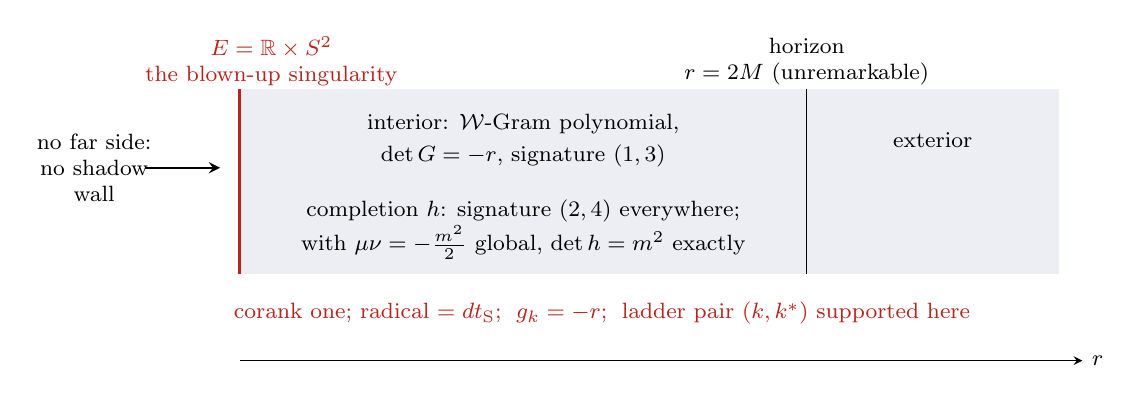
\begin{tikzpicture}[>=stealth,
  lab/.style={font=\footnotesize, align=center}]
\fill[MidnightBlue!8] (0,-1.35) rectangle (10.4,1.0);
\draw[very thick, BrickRed] (0,-1.35) -- (0,1.0);
\draw[thin] (7.2,-1.35) -- (7.2,1.0);
\node[lab, BrickRed] at (0.4,1.35) {$E = \R \times S^2$\\ the blown-up singularity};
\node[lab] at (7.2,1.35) {horizon\\ $r = 2M$ (unremarkable)};
\node[lab] at (3.6,0.55) {interior: $\shW$-Gram polynomial,};
\node[lab] at (3.6,0.15) {$\det G = -r$, signature $(1,3)$};
\node[lab] at (8.8,0.35) {exterior};
\node[lab, BrickRed] at (4.6,-1.85) {corank one; radical $= \dtS$;\; $g_k = -r$;\; ladder pair $(k, k^*)$ supported here};
\draw[->, thick] (-1.2,0.0) -- (-0.25,0.0);
\node[lab] at (-1.85,0.0) {no far side:\\ no shadow\\ wall};
\draw[->, thin] (0,-2.45) -- (10.7,-2.45) node[right, lab] {$r$};
\node[lab] at (3.6,-0.55) {completion $h$: signature $(2,4)$ everywhere;};
\node[lab] at (3.6,-0.95) {with $\mu\nu = -\tfrac{m^2}{2}$ global, $\det h = m^2$ exactly};
\end{tikzpicture}
\caption{The composite in one figure. The blow-up turns the worldline into the boundary hypersurface $E$; the weighted module absorbs the angular rates; the residual degeneration is corank one, first order, with the Killing-time direction as its radical. The completion ascends to $\Cl(2,4)$ on the whole manifold, the ladder pair is supported exactly on $E$, and the shadow wall, there being no far side, does not form.}
\label{fig:composite}
\end{figure}

\subsection{The exceptional algebra, the residue, and the Kasner weights}\label{subsec:schwexceptional}

\begin{proposition}[The exceptional algebra of the black hole]\label{prop:schwexceptional}
In the rescaled frame $(\rho,\, k/\sqrt{r},\, \mu_1,\, \mu_2)$ the Gram extends to $E$ with limit
\[
\mathrm{diag}(m^2,\, -1,\, -1,\, -1),
\]
nondegenerate of signature $(1,3)$; the cross term $G(\rho, k/\sqrt{r}) = -\sqrt{r}$ vanishes at the wall, and the dying entry $G(k/\sqrt r, k/\sqrt r) = -1$ is \emph{exact}, not merely limiting, being the rate of the degeneration. The exceptional algebra of the Schwarzschild singularity is $\Cl(1,3)$: the Clifford algebra of its Kasner form.
\end{proposition}

\begin{proposition}[The residue, and the square-root twist at the black hole]\label{prop:schwresidue}
$\displaystyle \lim_{r \to 0^+} r\,G^{-1} = -\,k \otimes k$, a rank-one limit; invariantly, the transversality datum $\delta : \shL^{\otimes 2} \to N^*_rE$ (the $r$-conormal line of the Conventions), $k \otimes k \mapsto -dr|_E$, is an isomorphism. The dying line, spanned on $E$ by the Killing-time covector, is a canonical square root of the $r$-conormal bundle of the singularity, and the partner line $\langle k^* \rangle$ adjoined by the completion is a canonical square root of its dual. The tautological twist of Theorem \ref{thm:residue} holds at the black hole, read in the $r$-graded conormal.
\end{proposition}

\begin{proof}[Proof of both]
The computations are short enough to print. In the rescaled frame, using Theorem \ref{thm:schwtame}'s Gram: $G(\rho, k/\sqrt r) = (G(\rho,\rho) + m\,G(\rho,\dtPG))/\sqrt r = ((m^2 - r) - m^2)/\sqrt r = -\sqrt r \to 0$, and $G(k/\sqrt r, k/\sqrt r) = g_k/r = -1$ exactly, so the limit Gram is $\mathrm{diag}(m^2, -1, -1, -1)$. For the residue, invert the $(\rho, \dtPG)$ block $\begin{psmallmatrix} m^2 - r & -m \\ -m & 1 \end{psmallmatrix}$, of determinant $-r$: the inverse is exactly $-\tfrac1r \begin{psmallmatrix} 1 & m \\ m & m^2 - r \end{psmallmatrix}$, so $r\,G^{-1} \to -\begin{psmallmatrix} 1 & m \\ m & m^2 \end{psmallmatrix} = -\,k \otimes k$ with $k = \rho + m\,\dtPG$, a rank-one matrix, while the angular block contributes $r \cdot O(1) \to 0$. All of this is confirmed as rational-function identities in the script; the invariance clauses are Lemma \ref{lem:invariantT2} and Theorem \ref{thm:residue}, applied one-sidedly per Remark \ref{rem:boundarytame} and read in $N^*_rE$ per the Conventions.
\end{proof}

\begin{theorem}[The weights are forced and are the Kasner exponents]\label{thm:weights}
Within the class of diagonal rescalings $r^{a_i}$ of the Schwarzschild coordinate coframe, demand that the rescaled cometric extend continuously to $E$. Then:
\begin{enumerate}
\item requiring a corank-one limit whose dying entry is the Killing-time entry, vanishing at first order, forces $(a_r, a_t, a_\theta) = (\tfrac12, 0, 1)$, uniquely: the degeneration-sheaf regime of Theorem \ref{thm:schwtame};
\item requiring a nondegenerate limit forces $(a_r, a_t, a_\theta) = (\tfrac12, -\tfrac12, 1)$, uniquely: the exceptional regime of Proposition \ref{prop:schwexceptional}.
\end{enumerate}
The naming of the dying entry in (1) is not a free choice but is read off the geometry: the radical of the actual degeneration is the Killing-time covector (Theorem \ref{thm:schwtame}(4)); without naming it, other slot assignments exist (for instance $(1, -\tfrac12, 1)$ sends the radial entry to zero at first order instead), so the forcing is per named profile. Converted to proper time $\tau_{\mathrm{p}} \propto r^{3/2}$, the exceptional weights are the Kasner exponents $(-\tfrac13, \tfrac23, \tfrac23)$ of Fact \ref{fact:kasner}, with $\sum p_i = \sum p_i^2 = 1$. This settles the Kasner-weights conjecture for Schwarzschild within the diagonal class: given the geometrically determined dying direction, the weights of the anisotropic completion are not chosen, they are forced, and they are the Kasner exponents.
\end{theorem}

\begin{proof}
The diagonal cometric entries have $r$-orders $(-1, +1, -2)$; a rescaling shifts these to $(2a_r - 1,\, 2a_t + 1,\, 2a_\theta - 2)$, and each regime's stated profile prescribes the target order of every slot ($(0, 1, 0)$ for the degeneration regime with the Killing-time slot dying, $(0,0,0)$ for the exceptional regime), determining each weight by the invertible linear relation displayed. The script confirms the two solutions by exhaustive search of the stated profiles over the grid $\tfrac16\mathbb{Z} \cap [-2,2]$ (a finite check of the linear solve, not a substitute for it) and verifies the conversion and the Kasner sum rules exactly.
\end{proof}

\subsection{Uniqueness of the weighted module}\label{subsec:uniqueness}

Proposition \ref{prop:Wframe} characterised $\shW$ operationally and fixed the quasihomogeneous order as the minimal one admitting a smooth frame. What it left open is whether some \emph{other} locally free extension of the interior cotangent module could carry a boundary-tame structure of its own. Within the rain-bounded class the answer is no, and the proof is short. Two explicit examples delimit the theorem exactly: first-order vanishing must be read on the dying eigenvalue, not the dying entry (Example \ref{ex:eigenentry}), and the rain-bounded hypothesis cannot be dropped, because null mixing produces genuinely different boundary-tame extensions outside it (Example \ref{ex:nullmix}).

\begin{definition}[Extensions]\label{def:extension}
An \emph{extension} is a locally free rank-four $C^\infty(\Mt_u)$-submodule $\mathcal{M}$ of the $u$-smooth one-forms which spans the full cotangent module over the interior and whose Gram $G|_{\mathcal{M}\times\mathcal{M}}$ extends smoothly to $E$. It is \emph{rain-bounded} if every element has bounded components in the infalling orthonormal frame, equivalently (Proposition \ref{prop:raindual}(3)) if $\mathcal{M} \subseteq \shW$. The boundary-tameness conditions are those of Remark \ref{rem:boundarytame}, with (T3$\partial$) read on the eigenvalue: the dying \emph{eigenvalue} of the Gram, with respect to any auxiliary frame metric, vanishes to exactly first order in the defining function $r$.
\end{definition}

\begin{theorem}[Uniqueness of the weighted module]\label{thm:uniqueW}
$\shW$ is the unique rain-bounded extension satisfying (T2$\partial$) and (T3$\partial$).
\end{theorem}

\begin{proof}
Let $\mathcal{M}$ be such an extension; rain-boundedness is exactly $\mathcal{M} \subseteq \shW$. By local freeness there is a transition matrix $A$ over $C^\infty(\Mt_u)$ expressing an $\mathcal{M}$-frame in the $\shW$-frame, invertible in the interior, and
\[
\det G_{\mathcal{M}} \;=\; (\det A)^2 \,\det G_{\shW} \;=\; -(\det A)^2\, r ,
\]
by Theorem \ref{thm:schwtame}(1). Fix a boundary point $x_0$. If $A(x_0, 0)$ is invertible then $A$ is invertible near $x_0$ and $\mathcal{M} = \shW$ there. If not, $\det A(x_0, u) \to 0$ as $u \to 0$, so $\det G_{\mathcal{M}}(x_0, u) = o(r)$. But by (T2$\partial$) exactly one eigenvalue of $G_{\mathcal{M}}$ vanishes at $x_0$ while the others are bounded away from zero, so the dying eigenvalue is $\det G_{\mathcal{M}}$ divided by a unit: it is $o(r)$, contradicting (T3$\partial$). Hence $A$ is invertible along all of $E$, and $\mathcal{M} = \shW$.
\end{proof}

\begin{example}[Rain-boundedness is essential: a null-mixing extension]\label{ex:nullmix}
Work on an angular chart and set $C := \tfrac12\sqrt{m^2 - u^2}$, $D := -\,m u^2/(2C)$, both $u$-smooth with $C(0) = m/2$. The module $\mathcal{M}'$ with frame
\[
\alpha = du + C\,d\theta, \qquad \beta = \dtPG + D\,d\theta, \qquad \gamma = u^4\,d\theta, \qquad \mu_2
\]
is a locally free rank-four extension in the sense of Definition \ref{def:extension}: its Gram extends smoothly to $E$, with
\[
\begin{gathered} G(\alpha,\alpha) = G(\alpha,\beta) = 0, \qquad G(\beta,\beta) = -\,\frac{u^2}{m^2 - u^2}, \\ G(\alpha,\gamma) = -C, \qquad G(\beta,\gamma) = -D, \qquad G(\gamma,\gamma) = -u^4 , \end{gathered}
\]
all exact. At the boundary the Gram has rank three with smooth radical spanned by $\beta$ (nonvanishing eigenvalues $\pm m/2$ from the $(\alpha,\gamma)$-pair and $-1$ from $\mu_2$), so (T2$\partial$) holds; and $\det G_{\mathcal{M}'} = -\,r/4$ exactly, so the dying eigenvalue is first-order in $r$ and (T3$\partial$) holds. Yet $\mathcal{M}' \neq \shW$: neither contains the other ($\alpha \notin \shW$, its rain component $\alpha(V) = -m/2u^2$ diverging; $\rho \notin \mathcal{M}'$). The mechanism is the null mixing of Remark \ref{rem:nullmixing}, and it shows the rain-bounded hypothesis of Theorem \ref{thm:uniqueW} is necessary, not technical. All displayed identities are verified exactly (Section \ref{sec:verification}).
\end{example}

\begin{corollary}[The characterisation is forced, within the rain-bounded class]\label{cor:forcedchar}
Within the rain-bounded class the characterisation of $\shW$ is not a choice of definition but a consequence of tameness: every rain-bounded boundary-tame extension is automatically the maximal one. The completion, the ladder pair, and the exceptional algebra of this section are therefore attached to the geometry together with the infalling congruence, whose finiteness class picks the module; Example \ref{ex:nullmix} shows some anchoring class must be named.
\end{corollary}

\begin{proof}
Let $\mathcal{M}$ be a rain-bounded boundary-tame extension. By Theorem \ref{thm:uniqueW}, $\mathcal{M} = \shW$; and $\shW$ is the maximal rain-bounded extension because rain-boundedness is, by Definition \ref{def:extension} and Proposition \ref{prop:raindual}(3), exactly the inclusion $\mathcal{M} \subseteq \shW$. The remaining clauses restate Theorems \ref{thm:schwcompletion} and \ref{thm:uniqueW} and Example \ref{ex:nullmix}.
\end{proof}

\begin{example}[The eigenvalue is essential]\label{ex:eigenentry}
Fix $c \neq 0$ and let $\mathcal{M}_c \subset \shW$ be generated by $(u\rho,\ k + c\rho,\ \mu_1,\ \mu_2)$, with $k = \rho + m\,\dtPG$ the radical section. Then $\mathcal{M}_c$ is a strict submodule (its boundary evaluation has rank three), it satisfies (T2$\partial$), and its dying \emph{entry} is
\[
G(u\rho,\,u\rho) \;=\; r\,(m^2 - r) :
\]
first order in $r$, with nonvanishing coefficient. Nevertheless its dying \emph{eigenvalue} is second order: $\det A = mu$, so $\det G_{\mathcal{M}_c} = -m^2 r^2$ exactly, while the nonvanishing $3\times 3$ minor at the boundary equals $c^2 m^2 \neq 0$: the off-diagonal entries of order $u$ reduce the first-order diagonal entry to a second-order eigenvalue. So $\mathcal{M}_c$ is corank one with a first-order dying entry and is \emph{not} $\shW$: the entry formulation of (T3$\partial$) would make Theorem \ref{thm:uniqueW} false, and the eigenvalue formulation is the correct one. All displayed identities are verified exactly (Section \ref{sec:verification}).
\end{example}

\subsection{The rain frame: the physical meaning of the module}\label{subsec:rainframe}

The weighted module has, so far, been characterised metrically (bounded norm) and structurally (uniqueness). It also has an operational characterisation, and the structure behind it is a duality with the exceptional regime. Let $(V, e_{\hat r}, e_{\hat\theta}, e_{\hat\phi})$ be the infalling orthonormal frame of the Painlev\'e-Gullstrand form of Fact \ref{fact:pg}: $V = \partial_t - \beta\partial_r$ the rain four-velocity, $e_{\hat r} = \partial_r$, and the unit sphere directions; its exact orthonormality at every radius is itself one of the machine checks.

\begin{proposition}[Rain duality]\label{prop:raindual}
At every interior radius, exactly:
\begin{enumerate}
\item the coframe $(\dtPG,\ k/\sqrt r,\ \mu_1,\ \mu_2)$ is the \emph{dual coframe} of the infalling orthonormal frame: the pairing matrix is the identity, the vanishing $(k/\sqrt r)(V) = 0$ being the rain identity of Theorem \ref{thm:schwtame}(5);
\item its Gram is exactly Minkowski, $\operatorname{diag}(1,-1,-1,-1)$, at every radius, horizon and collar included: $\dtPG$, the Painlev\'e-Gullstrand time, is the rain's proper-time differential, and the rain observer's covector space never degenerates;
\item a $u$-smooth one-form lies in $\shW$ if and only if its rain-frame components are bounded up to the singularity; the norm identity $|\alpha|_G^2 = \alpha(V)^2 - \sum_i \alpha(e_{\hat\imath})^2$ holds exactly, though boundedness of the norm alone does not suffice for membership (Remark \ref{rem:nullmixing}); the excluded coordinate forms diverge, $dr(V) = -m/\sqrt r$ and $d\theta(e_{\hat\theta}) = 1/r$;
\item the module $\shW_{\mathrm{exc}}$ spanned by the coframe of (1) over $C^\infty(\Mt_u)$ is the exceptional-regime module of Proposition \ref{prop:schwexceptional}; rain-frame components of a covector are precisely its $\shW_{\mathrm{exc}}$-coefficients; and $\shW \subset \shW_{\mathrm{exc}}$, via $\rho = \sqrt r\,(k/\sqrt r) - m\,\dtPG$, with transition determinant $-\sqrt r$. The weighted module is the $u$-smooth shadow of the rain observer's covector space, and the degeneration-regime/exceptional-regime dichotomy of Theorem \ref{thm:weights} is the dichotomy between the blow-up's smooth structure and the rain frame.
\end{enumerate}
\end{proposition}

\begin{proof}
All clauses are exact rational-function identities, verified at two masses, the angular clauses at the equator; general position is literally the same algebra, since $\sin\theta$ enters $\mu_2$ and $e_{\hat\phi}$ reciprocally and cancels identically in every pairing and Gram entry used (Section \ref{sec:verification}). (1) is the pairing table: $\dtPG(V) = 1$, $(k/\sqrt r)(e_{\hat r}) = 1$, $\mu_i(e_{\hat\imath}) = 1$, all others zero. (2): $G(\dtPG,\dtPG) = 1$, $G(\dtPG, k/\sqrt r) = 0$, $G(k/\sqrt r, k/\sqrt r) = g_k/r = -1$ exactly, by Theorem \ref{thm:schwtame}. (3): membership in $\shW$ gives bounded components by (1) applied to the frame. Conversely, write $\alpha = A\,du + B\,dt + C'\,d\theta + D'\sin\theta\,d\phi$ with $u$-smooth coefficients: boundedness of $\alpha(e_{\hat r}) = A/(2u)$ forces $A = O(u)$, then boundedness of $\alpha(V) = B - mA/(2u^2)$ forces $A = O(u^2)$, and boundedness of the angular components $C'/u^2$, $D'/u^2$ forces $C', D' = O(u^2)$; a $u$-smooth function that is $O(u^2)$ is $u^2$ times a $u$-smooth function (Taylor division), so $\alpha$ is a $C^\infty(\Mt_u)$-combination of $\rho$, $dt$, $\mu_1$, $\mu_2$: $\alpha \in \shW$. The norm identity itself is the statement that the frame of (1) is $G$-orthonormal, i.e.\ clause (2). (4): the displayed transition and its determinant $\det\begin{psmallmatrix} -m & \sqrt r\\ 1 & 0\end{psmallmatrix} = -\sqrt r$; the frame comparison with Proposition \ref{prop:schwexceptional} replaces the timelike leg $\rho$ by $\dtPG$ through the same transition.
\end{proof}

\begin{proposition}[The chain's radial dyad is rain-finite]\label{prop:dyad}
Let $n_\pm := k/\sqrt r \pm \dtPG$. Then, at every interior radius, exactly: $n_\pm$ are $G$-null; they are $\shW_{\mathrm{exc}}$-sections with \emph{constant unit} rain components, $n_\pm(V) = \pm 1$ and $n_\pm(e_{\hat r}) = 1$; and the gauge field of Fact \ref{fact:pg} carries the flat radial null dyad onto them,
\[
L^{-1}(\dtPG + dr) \;=\; n_+, \qquad L^{-1}(\dtPG - dr) \;=\; -\,n_- ,
\]
where $L$ is the covector action of the gauge field, fixed internally by the identity $\eta(L a, L b) = G(a,b)$ on all coordinate pairs. Hence the s-wave sector's physical null dyad, the radial structure on which the chain of \cite{ButlerT5} runs, is exactly finite in the infalling frame all the way to the wall, even though the individual coordinate legs are not.
\end{proposition}

\begin{proof}
Nullity: $G(n_\pm, n_\pm) = -1 + 1 = 0$ by Proposition \ref{prop:raindual}(2). Components: clause (1) of the duality. The gauge map $L(\dtPG) = \dtPG$, $L(dr) = dr - \beta\,\dtPG$, angular fixed, satisfies $\eta(La, Lb) = G(a,b)$ on all coordinate pairs, which fixes the conventions internally; inverting, $L^{-1}(\dtPG \pm dr) = (1 \pm \beta)\dtPG \pm dr = \pm\bigl(dr + (\beta \pm 1)\dtPG\bigr) = \pm\,n_\pm$. All identities exact, at two masses (Section \ref{sec:verification}).
\end{proof}

\begin{remark}[The kinematic status of the module]\label{rem:rainanswer}
At the singular boundary the raw cotangent module is not a carrier: it admits no bounded extension across $E$ (the order-one structure fails the minimality clause of Proposition \ref{prop:Wframe}), and by Theorem \ref{thm:uniqueW} the rain-bounded boundary-tame extension is unique. The positive identification is two-tier: what the infalling observer measures finitely is exactly the exceptional module, the nondegenerate rain-dual carrier; its $u$-smooth shadow is $\shW$, the tame carrier of the degeneration sheaf; and the chain's own radial dyad lies in the former with constant unit components. The exceptional algebra of Proposition \ref{prop:schwexceptional} is, literally, the Clifford algebra of what the rain measures. What remains interpretive is confined to the operator and state level of \cite{ButlerT5}'s chain, and is recorded in Section \ref{subsec:schwscope}.
\end{remark}

\subsection{The matching with the weighted limit}\label{subsec:weld}

The weighted-limit paper reaches the same singularity at tractor level. This subsection proves that the two routes meet in one structure: the exceptional bundle of this section, transported.

\begin{fact}[The weighted limit]\label{fact:weightedlimit}
In the Schwarzschild interior with $2M = 1$: the metric takes the synchronous form $d\tau^2 - A\,dt^2 - r^2 d\Omega^2$, $A = (1-r)/r$, with $\tau = \tfrac23 r^{3/2}(1 + \tfrac{3}{10}r + O(r^2))$; the orthonormal frame adapted to $(t, \theta, \varphi)$ is exactly parallel along $\partial_\tau$; its Hubble-normalised expansion rates are $\tau\sigma_1 = -\tfrac13 - \tfrac{4}{15}R + O(R^2)$ and $\tau\sigma_2 = \tau\sigma_3 = \tfrac23 - \tfrac{2}{15}R + O(R^2)$, $R = (3\tau/2)^{2/3}$; the connection on unit tangential directions is $\Omega(e_i) = \sigma_i B_i$ plus a sphere term of size $O(1/r)$, with $B_i$ the boosts; and for every admissible synchronous metric (Einstein, $\mathrm{Ric} = \Lambda g$ with $\Lambda$ constant; Hubble-normalised connection $\sum_i p_iB_i \otimes \hat\theta^i + E_\tau$ with \emph{constant} $p_i \neq 0$, $E_\tau \to 0$, and $\|E_\tau\|/\tau$ integrable, both locally uniformly on the boundary base) the weighted limit exists, equals $\widehat\Omega_0 = \sum_i p_i B_i \otimes \hat\theta^i$, extends the parallel tractor, and has boundary holonomy exactly $\mathfrak{so}(1,3)$ in the values-level sense of \cite[Def.~5.5]{ButlerT6} (the algebra generated by the limiting connection values). \emph{Provenance:} \cite{ButlerT6}, Lemmas 5.1-5.4, Definition 5.5, and Theorem 5.6.
\end{fact}

\begin{proposition}[The matching at the fibre]\label{prop:fibreweld}
Normalise the exceptional Gram to $\eta = \operatorname{diag}(1,-1,-1,-1)$, with $\hat e_0$ the proper-time direction and $\hat e_i$ the Kasner eigendirections. Then: (1) the bivector algebra of the exceptional fibre is $\mathfrak{so}(1,3)$, the holonomy algebra of Fact \ref{fact:weightedlimit}, and the identification of the two fibres matching proper time, eigendirections, and exponents is canonical up to the isometries preserving the Kasner data; (2) under it, the surviving matrix $\sum_i p_i B_i$ corresponds to the \emph{weight bivector} $B_w = \sum_i p_i\,\hat e_0 \wedge \hat e_i$, because the weights of the sheaf construction are forced to equal the exponents (Theorem \ref{thm:weights}); (3) $B_w$ is $\eta$-antisymmetric with characteristic polynomial $\lambda^4 - (\sum_i p_i^2)\lambda^2 = \lambda^4 - \lambda^2$: \emph{the second Kasner relation says precisely that the surviving matrix is a unit boost of the exceptional algebra}. The wall itself carries the transverse generator: the ladder boost $K = \tfrac12[k,k^*] = k \wedge k^* = N - \tfrac12$ (no relation to the exterior form $K$ of Theorem \ref{thm:absolute}), with $K^2 = \tfrac14$ on the whole ambient fibre, an $\mathfrak{so}(1,1)$ supported on the wall.
\end{proposition}

\begin{proof}
(1): the map $x \wedge y \mapsto \bigl(z \mapsto \eta(x,z)\,y - \eta(y,z)\,x\bigr)$ sends bivectors to $\eta$-antisymmetric endomorphisms, is injective (a nonzero bivector moves some vector), and both spaces have dimension six, so the bivector algebra of the exceptional fibre \emph{is} $\mathfrak{so}(1,3)$, with the commutator matching the Clifford bracket; the script checks closure, dimension, and the bracket exactly. The residual freedom for $p_2 = p_3$ is the $O(2)$ of the degenerate pair. (2) is the dictionary: both sides attach the same exponents to the same eigendirections, by Theorem \ref{thm:weights} here and by definition there. (3): the action of $B_w$ sends $\hat e_0 \mapsto \sum_i p_i \hat e_i$ and $\hat e_j \mapsto p_j\, \hat e_0$, so it vanishes on the spatial vectors orthogonal to $\hat p := \sum_i p_i \hat e_i$ and squares to $\sum_i p_i^2$ times the identity on the boost plane $\operatorname{span}\{\hat e_0, \hat p\}$: the characteristic polynomial is $\lambda^2\,(\lambda^2 - \sum_i p_i^2) = \lambda^4 - (\sum_i p_i^2)\lambda^2$, and the constraint $\sum p_i^2 = 1$ normalises it (the script confirms the polynomial at two rational Kasner points). The ladder identities $K = N - \tfrac12$ and $K^2 = \tfrac14$ are verified on all $64$ ambient states (Section \ref{sec:verification}).
\end{proof}

\begin{theorem}[The matching at connection level]\label{thm:connweld}
In the Schwarzschild interior, write $(d\tau, \theta^1, \theta^2, \theta^3)$ for the adapted orthonormal coframe of Fact \ref{fact:weightedlimit} (synchronous time, normalised Killing direction, sphere directions). Then:
\begin{enumerate}
\item \emph{(Frames.)} The adapted coframe consists of exceptional-module sections, exactly: $\sqrt{m^2 - r}\;d\tau = \rho$ and
\[
\sqrt{m^2 - r}\;\theta^1 \;=\; -\sqrt r\,\dtPG \,+\, m\,(k/\sqrt r),
\]
with $\theta^2 = \mu_1$, $\theta^3 = \mu_2$ exactly (the first identity uses the transition of Theorem \ref{thm:schwtame}(4)). The static and rain frames of $\shW_{\mathrm{exc}}$ are related by the boost of rapidity $\chi$ with $(\sinh\chi, \cosh\chi) = (-\sqrt r, m)/\sqrt{m^2-r}$, unit-normalised exactly and vanishing on the exceptional boundary: the two frames coincide at the wall, future orientations matched.
\item \emph{(Rates.)} In this common frame the Hubble-normalised connection is $\sum_i (\tau\sigma_i)B_i \otimes \hat\theta^i$ plus a sphere term of normalised size $\tau/r = \tfrac23\sqrt r + O(r^{3/2}) \to 0$, with the exact series of Fact \ref{fact:weightedlimit} re-derived here independently by exact power series in $\sqrt r$, agreeing coefficient by coefficient, and the trace rule $\tau(\sigma_1 + 2\sigma_2) \to 1$ realising the first Kasner relation as a rate statement.
\item \emph{(The matching.)} Consequently the weighted-limit connection of Fact \ref{fact:weightedlimit} is a connection datum on the exceptional bundle of this section: its boundary value is the weight one-form $\sum_i p_i B_i \otimes \hat\nu^i$ of the exceptional coframe, its total element is the unit boost $B_w$ of Proposition \ref{prop:fibreweld}, and its values, nonzero multiples of the three boosts, generate the full bivector algebra, so the holonomy theorem of \cite{ButlerT6} is the statement that the boundary holonomy of the exceptional bundle, in the values-level sense of \cite[Def.~5.5]{ButlerT6}, is all of $\mathfrak{so}(1,3)$; the matching uses exactly those values. The two black-hole routes are one structure: the weighted limit transports the exceptional fibre, the completion Clifford-multiplies it, and the ladder boost is the transverse $\mathfrak{so}(1,1)$.
\end{enumerate}
\end{theorem}

\begin{proof}
(1) The rationalised identities are exact: $\sqrt{m^2-r}\,d\tau = \sqrt{m^2-r}\,\sqrt{r/(m^2-r)}\,dr = \rho$, and multiplying $\theta^1 = \sqrt{(m^2-r)/r}\;\dtS$ by $\sqrt{m^2-r}$ and substituting the transition of Theorem \ref{thm:schwtame}(4) gives componentwise $((m^2-r)/\sqrt r)\,\dtPG + m\,dr$, which equals $-\sqrt r\,\dtPG + m(k/\sqrt r)$; both are verified as rational-function identities at two masses, along with the unit-boost identity and $G(d\tau,d\tau) = 1$. The boundary limit: the coefficients $(-\sqrt r, m)/\sqrt{m^2-r} \to (0,1)$, so $\theta^1 \to k/\sqrt r$, and $\rho \to -m\,\dtPG$ in $\shW_{\mathrm{exc}}$ gives $d\tau \to -\dtPG$: after matching the future orientations of the two congruences the frames agree on the boundary. (2) The frame is that of Fact \ref{fact:weightedlimit}, so the connection is its display; the series are re-derived independently: $\tau(r) = \int_0^r \sqrt{s/(1-s)}\,ds$, $\sigma_1 = -\tfrac12 r^{-3/2}(1-r)^{-1/2}$, $\sigma_2 = r^{-3/2}(1-r)^{1/2}$, manipulated as exact truncated power series in $\sqrt r$, reproducing the printed constants $-\tfrac13, -\tfrac{4}{15}, \tfrac23, -\tfrac{2}{15}$ (Section \ref{sec:verification}). (3) is the assembly of (1), (2), and Proposition \ref{prop:fibreweld}, with the fullness argument imported from Fact \ref{fact:weightedlimit}, whose inputs are exactly the nonvanishing $p_i$ and the bracket structure verified here.
\end{proof}

\begin{remark}[What remains of the matching]\label{rem:weldopen}
Fact \ref{fact:weightedlimit}'s admissibility fixes \emph{constant} Kasner exponents, so Theorem \ref{thm:connweld} matches the routes for the constant-exponent admissible class, Schwarzschild included. The variable-exponent generalisation of the weighted limit theorem, the connection-level analogue of Section \ref{sec:anisotropic}, is the single remaining ingredient of a fully matched singular boundary; its Gram-level half is Section \ref{sec:anisotropic}, and its connection-level half is a Duhamel argument in the variable-order structure, expected but not attempted here.
\end{remark}

\subsection{Consequences, and what remains open}\label{subsec:schwscope}

\emph{The localisation import of the singularity paper.} The singularity paper \cite{ButlerT5} imports this paper's localisation for a case that failed the tame hypotheses. For exact Schwarzschild this section supplies the missing structure: the ascent and the ladder pair are theorem-backed \emph{at the black hole}, localised on $E \cong \R \times S^2$, in the boundary-tame weighted sense defined here. Separately, the corank ambiguity behind the count of boundary modes at the singularity (corank $1$, $2$ or $3$ depending on rescaling weight) is resolved structurally: with the weights of Theorem \ref{thm:weights}, forced once the dying direction is read off the geometry, the corank is exactly one, so there is one ladder pair per point of $E$, not one per dying coordinate direction. What this section does \emph{not} do is compute the quantitative content of the boundary mode space: the epoch and count analysis belongs to \cite{ButlerT8}, and the aggregation over the sphere factor of $E$ is exactly the slice-to-epoch question assigned to that paper.

\emph{The conservation principle.} The constant-determinant global completion of Remark \ref{rem:schwconservation} is the first explicit example exhibiting the sharpness of Theorem \ref{thm:absolute}'s standardness hypothesis, and the boundary case completes the trichotomy: interior wall, shadow wall; boundary wall, no wall; non-standard completion, wall at infinity.

\emph{What remains open.} Four problems, at the boundary of what this paper's methods reach. \textbf{The analysis of the anisotropic class}: Section \ref{sec:anisotropic} closes the diagonal class at the algebraic level, position-dependent exponents included, stably under relatively admissible errors, with the smooth structure of the function algebra characterised in Section \ref{subsec:smoothstructure} and the collision boundary settled in Section \ref{subsec:collisions}; what it does not supply is analysis: the dictionary identifying the connection-level admissibility of \cite{ButlerT6} with Gram-level relative admissibility for genuine velocity-dominated solutions, and the dynamical traversal of the Taub edges, the bounce and era maps themselves, both of which lie in \cite{ButlerT6}'s admissibility class. \textbf{Kerr}: the ring has codimension two and, unlike every case treated here, a lightlike dying direction (see Section \ref{subsec:scope}); the Kerr composite, on a twisted variable-order module over a focal double cover, is the genuine successor problem, and its geometry is assigned to \cite{ButlerT6}. \textbf{The operator and state level}: Section \ref{subsec:rainframe} answers the kinematic question of what $\shW$ is, the $u$-smooth shadow of what the infalling observer measures finitely; whether the fermionic modes and modular structures of the boundary mode space of \cite{ButlerT5}'s chain, built on the dyad shown there to be rain-finite, define states on the completion at the wall is a question for \cite{ButlerT5}'s framework. \textbf{The variable-exponent weighted limit}: Section \ref{subsec:weld} matches the weighted limit of \cite{ButlerT6} to the present construction at the fibre and at the connection level; extending the matching to position-dependent exponents is the question posed precisely in Remark \ref{rem:weldopen}.

\section{The anisotropic class: variable weights and stability}\label{sec:anisotropic}

The Schwarzschild composite used constant Kasner exponents. The general velocity-dominated case has exponents varying over the singular surface. This section closes the algebraic half of that problem. The principle that makes it tractable is worth stating once: \emph{every tame-wall construction of this paper is $C^\infty$-linear}. The degeneration sheaf, the ideal, the coupling, the completion, the ladder pair, the exceptional rescaling: every construction is algebra-linear in the coefficient functions and never differentiates them. Position-dependent exponents therefore affect only the \emph{function algebra} over which the module is defined, never the constructions performed over it.

\begin{definition}[Variable-order algebra; strict diagonal data]\label{def:varorder}
Let $E$ be a smooth $3$-manifold and $\Mt = [0,\varepsilon)_\tau \times E$. An \emph{admissible exponent family} is a countable family $\{e_j\}$ of smooth nonnegative functions on $E$ such that, on each compact $K \subseteq E$ and for each level $N$, only finitely many $e_j$ have $\inf_K e_j \leq N$. The \emph{variable-order algebra} $\mathcal{A}$ is the algebra of sums $\sum_j f_j(x,\tau)\,\tau^{e_j(x)}$ over admissible exponent families, with $f_j$ smooth up to $\tau = 0$; on each compact and each interval $[0, \tau_0]$, the terms below any level are finitely many and the remainder is $O(\tau^{N})$ locally uniformly, so the sums converge locally uniformly and the class is closed under products (exponent families add, and the sum family is again admissible). Two conventions: an element is identified with the function it defines, and the representation-sensitive notions used later (exponent sets, log degree) rest on the non-membership statements of Section \ref{subsec:smoothstructure}, which are proved for exactly this class. \emph{Strict diagonal data} on $\Mt$ is a local coframe $(d\tau, \sigma^1, \sigma^2, \sigma^3)$ and a cometric whose Gram in it is
\[
\operatorname{diag}\bigl(1,\ -\tau^{-2p_1(x)}c_1,\ -\tau^{-2p_2(x)}c_2,\ -\tau^{-2p_3(x)}c_3\bigr),
\]
with $p_i$ smooth, $p_1 < 0 < p_2 \leq p_3$ pointwise, and $c_i(x,\tau)$ smooth and positive up to $\tau = 0$. The Kasner constraints are \emph{not} hypotheses of anything in this section: the sheaf theory is kinematic, and the constraints enter only through the Einstein-flow provenance of Fact \ref{fact:kasner}.
\end{definition}

\begin{lemma}[Boundary units invert]\label{lem:units}
If $a \in \mathcal{A}$ has every exponent bounded below by some $\delta > 0$ on the relevant compact (so $a = O(\tau^\delta)$ locally uniformly), then $1 + a$ is invertible in $\mathcal{A}$ after shrinking $\varepsilon$: the Neumann series $\sum_{k \geq 0} (-a)^k$ has exponent families adding to $\{k\delta + \cdots\}$, admissible since only finitely many products fall below any level, and it converges locally uniformly where $|a| \leq \tfrac12$. More generally any $c + a$ with $c$ smooth, positive and bounded away from zero near $E$ is invertible in $\mathcal{A}$.
\end{lemma}

\begin{proof}
Admissibility of the summed family: a product of $k$ factors from $a$'s family has exponent at least $k\delta$ on the compact, so for each level $N$ only the terms with $k \leq N/\delta$, finitely many products each, can lie below $N$. Local uniform convergence is the geometric bound. The general case is $c + a = c(1 + a/c)$, with $a/c \in \mathcal{A}$ of the same positive lower order ($1/c$ is smooth up to the boundary).
\end{proof}

\begin{theorem}[Variable-weight boundary tameness, completion, forced weights]\label{thm:varexp}
For strict diagonal data, let $\shW$ be the $\mathcal{A}$-module with frame $\vartheta_0 = d\tau$, $\vartheta_1 = \sigma^1$, $\vartheta_2 = \tau^{p_2(x)}\sigma^2$, $\vartheta_3 = \tau^{p_3(x)}\sigma^3$ (the letter avoiding the coupling constant $\nu$). Then:
\begin{enumerate}
\item $\shW$ is free of rank four over $\mathcal{A}$, with Gram $\operatorname{diag}(1, -\varrho c_1, -c_2, -c_3)$, $\varrho := \tau^{-2p_1(x)} \in \mathcal{A}$, extending to $E$ with corank exactly one; the radical is the line of the negative-exponent covector $\sigma^1$, and the dying entry is $-\varrho c_1$: exactly first order in the canonical defining element $\varrho$.
\item The one-sided completion applies verbatim: coupling to the dying direction with $\mu\nu < 0$ yields signature $(2,4)$ on a collar, boundary included, with the ladder pair supported exactly on $E$ and no shadow wall ($s = -1/(\varrho c_1) < 0$ throughout, so $F \geq 1$ wherever the bump is supported); the global coupling $\mu\nu = -\tfrac12$ has $\det h = c_2c_3(1 + \varrho c_1)$, nonvanishing everywhere on the collar.
\item The weights are forced pointwise: within diagonal rescalings $\tau^{a_i(x)}$, the corank-one regime \emph{with the negative-exponent axis dying at first order in $\varrho$} forces $(a_0,\dots,a_3) = (0,0,p_2,p_3)$, and the nondegenerate regime forces $(0,p_1,p_2,p_3)$: the local exponents, at each point separately. (As at Schwarzschild, naming the dying axis is read off the geometry, the negative-exponent covector being the radical of the actual degeneration; without naming it other slot assignments exist.) The exceptional Gram is $\operatorname{diag}(1,-c_1,-c_2,-c_3)|_{\tau=0}$, a smooth bundle of nondegenerate $(1,3)$ forms over $E$: the Clifford algebras of the local Kasner forms.
\end{enumerate}
Consequently the degeneration sheaf, the square-zero ideal with quotient $\Cl(1,2)$, the localised ladder pair, and the exceptional algebra all exist with position-dependent exponents, by the $C^\infty$-linearity of their constructions applied fibrewise.
\end{theorem}

\begin{proof}
(1) Freeness: a relation $\sum c_i\vartheta_i = 0$ has interior coefficients $c_0, c_1, c_2\tau^{p_2}, c_3\tau^{p_3}$ against the coframe, all forced to vanish where $\tau > 0$, hence identically. The Gram entries: $\vartheta_2$ carries $\tau^{2p_2}(-\tau^{-2p_2}c_2) = -c_2$, likewise $\vartheta_3$; and $\varrho \in \mathcal{A}$ since $-2p_1 > 0$ pointwise. Corank and radical are read off the boundary values $\operatorname{diag}(1, 0, -c_2, -c_3)$. (2) The coupling construction is a pointwise modification of the Gram by elements of $\mathcal{A}$ and constants; the determinant identity of Lemma \ref{lem:det} is algebraic, valid over any commutative ring, with $s = G^{-1}(e,e) = -1/(\varrho c_1)$ here; the boundary signature is Lemma \ref{lem:wallgram} with $\mu\nu < 0$; the global determinant is the same identity at $\beta \equiv 1$. (3) The diagonal entries have $\tau$-orders $(0, -2p_1, -2p_2, -2p_3)$; each regime's named profile prescribes the target order of every slot, and the resulting equations are linear with the displayed unique solutions. All computational clauses are verified as exact rational-function identities at three rational Kasner points, with the ladder pair on all $64$ boundary states (Section \ref{sec:verification}).
\end{proof}

\subsection{Stability under relatively admissible errors}\label{subsec:stability}

True velocity-dominated solutions are diagonal only to leading order \cite{IsenbergMoncrief1990}. The error structure the asymptotics deliver is \emph{relative}: each Gram entry is its model value times $1 + o(1)$, and each off-diagonal entry is small relative to the geometric mean of the two scales it couples. The following definition transcribes that structure onto the weighted frame, where the nondegenerate scales are units and the dying scale is $\varrho$.

\begin{definition}[Relatively admissible perturbation]\label{def:reladm}
Let $G$ be the weighted Gram of Theorem \ref{thm:varexp}, dying slot $1$, nondegenerate slots $\{0,2,3\}$. A symmetric $\mathcal{A}$-bilinear perturbation $\Xi_\bullet$ (the letter avoiding the boundary $E$) is \emph{relatively admissible} if, for some $\delta > 0$: the entries on the nondegenerate slots lie in $\tau^\delta\mathcal{A}$; the mixed entries (dying slot against a nondegenerate slot) lie in $\varrho^{1/2}\tau^\delta\mathcal{A}$ (note $\varrho^{1/2} = \tau^{-p_1(x)} \in \mathcal{A}$); and the dying entry lies in $\varrho\,\tau^\delta\mathcal{A}$.
\end{definition}

\begin{theorem}[Stability: reduction to the strict-diagonal case]\label{thm:stability}
For every relatively admissible $\Xi_\bullet$, the perturbed pair $(\shW, G + \Xi_\bullet)$ is congruent, by a transition in $GL_4(\mathcal{A})$ which is the identity on the exceptional boundary, to diagonal data over $\mathcal{A}$ with the \emph{same} exponents and perturbed unit entries $c_i' = c_i(1 + O(\tau^\delta))$, boundary units of $\mathcal{A}$ in the sense of Lemma \ref{lem:units} (smoothness of the units is not preserved, membership in $\mathcal{A}$ is). Consequently every conclusion of Theorem \ref{thm:varexp} holds verbatim for the perturbed data: the same module, corank one with the same radical, dying eigenvalue of exactly first order in $\varrho$ with the unperturbed leading unit, the $(2,4)$ completion with no shadow wall, and the same pointwise-forced weights.
\end{theorem}

\begin{proof}
The nondegenerate $3\times3$ block $H' = H + \Xi_H$ has determinant a boundary unit, so symmetric Gaussian elimination diagonalises it congruently over $\mathcal{A}$ with a unit transition: each pivot is a boundary unit plus $\tau^\delta\mathcal{A}$, invertible in $\mathcal{A}$ by Lemma \ref{lem:units}. The dying-slot cross column $b$ has entries in $\varrho^{1/2}\tau^\delta\mathcal{A}$, so $x := H'^{-1}b$ lies in the same class, and the block congruence by $\mathrm{id}$ minus the column $x$ into slot $1$ eliminates it exactly, leaving the Schur complement
\[
\tilde d \;=\; G_{11} + \Xi_{11} - b^{\mathsf T}H'^{-1}b \;=\; -\varrho c_1 + \varrho\,\tau^\delta(\cdots) + \varrho\,\tau^{2\delta}(\cdots) \;=\; -\varrho\,c_1\bigl(1 + O(\tau^\delta)\bigr),
\]
the last term because the cross column's square carries $(\varrho^{1/2}\tau^\delta)^2 = \varrho\tau^{2\delta}$. The total transition is a product of unit transitions, hence a unit, and the result is diagonal data over $\mathcal{A}$ with perturbed unit entries; every conclusion quoted from Theorem \ref{thm:varexp} used only that the units are positive boundary units of $\mathcal{A}$, never their smoothness. The congruence is executed explicitly in the verification script at a rational Kasner point with a concrete relatively admissible perturbation: cross-term elimination, the Schur identity, the preserved first-order eigenvalue with leading unit $-1$, corank and radical, and the perturbed completion's determinant identity, nonvanishing boundary determinant, and $(2,4)$ signatures.
\end{proof}

\begin{example}[Sharpness at relative order zero]\label{ex:sharp}
The strict positivity $\delta > 0$ is necessary, not technical. Take the mixed error $\Xi_{12} = c\,\varrho^{1/2}$ on the dying-nondegenerate slot pair, relative order exactly zero. The Schur correction is then of order $\varrho$ and adds to the leading unit: in the verified example the choice $c = 2$ keeps the eigenvalue at first order but flips its leading unit from $-1$ to $+3$, changing the sign structure of the wall, while the choice $c = 1$ cancels the leading term entirely and the dying eigenvalue jumps to the \emph{square} of the defining order. At relative order zero the first-order structure is coefficient-dependent, hence not stable; below it, Theorem \ref{thm:stability} says it is unaffected.
\end{example}

\subsection{The smooth structure of the variable-order algebra}\label{subsec:smoothstructure}

Definition \ref{def:varorder} introduced $\mathcal{A}$ by fiat, and it is natural to ask whether it is the function ring of a variable-order polyhomogeneous structure in the sense of \cite{Melrose1993}. This subsection answers the question. The answer is yes, at the cost of logarithms, and the cost is provably unavoidable: the algebra is stable under the boundary calculus in the radial direction, fails stability in the tangential directions by an exactly computable logarithmic term, and no admissible change of collar presentation removes the failure unless the exponent ratios are constant.

\begin{lemma}[The log obstruction]\label{lem:logobstruction}
For $e$ smooth on $E$,
\[
\tau\partial_\tau\,\tau^{e(x)} \;=\; e(x)\,\tau^{e(x)},
\qquad
\partial_x\,\tau^{e(x)} \;=\; e'(x)\,\tau^{e(x)}\log\tau .
\]
Consequently $\mathcal{A}$ is a commutative algebra stable under $\tau\partial_\tau$; it is stable under tangential vector fields if and only if every exponent is locally constant; and the obstruction is genuine: if $e'(x_0) \neq 0$ then $\tau^{e(x)}\log\tau$ does not lie in $\mathcal{A}$ near $(x_0,0)$.
\end{lemma}

\begin{proof}
The displayed formulas are the chain rule on $\tau^e = \exp(e\log\tau)$. For the non-membership, fix $x = x_0$, write $e_0 := e(x_0)$, and suppose $\tau^{e_0}\log\tau = \sum_j g_j(\tau)\,\tau^{c_j}$ with $g_j$ smooth and $\{c_j\}$ an admissible exponent family evaluated at $x_0$: distinct reals, only finitely many below any level. Absorb the finitely many terms with $c_j = e_0$ into the left side and divide by $\tau^{e_0}$:
\[
\log\tau - g(\tau) \;=\; \sum_j g_j(\tau)\,\tau^{d_j}, \qquad d_j := c_j - e_0 \ \text{distinct and nonzero},
\]
with $g$ smooth. Split the right side into the positive part $P$ ($d_j > 0$: finitely many terms below level $1$ plus an $O(\tau)$ tail, so $P = o(1)$) and the negative part $R$ ($d_j < 0$: finitely many terms, by admissibility). Then $R = \log\tau + O(1)$, so in particular $R = o(\tau^{-\varepsilon})$ for every $\varepsilon > 0$. We raise the exponents of $R$ one at a time. Let $d_{\min} < 0$ be the least exponent present in $R$; every term of $\tau^{|d_{\min}|} R = \sum g_j \tau^{d_j + |d_{\min}|}$ has nonnegative exponent, so it extends continuously to $\tau = 0$ with limit $g_{j_0}(0)$, where $j_0$ is the (unique, exponents being distinct) index with $d_{j_0} = d_{\min}$. But $\tau^{|d_{\min}|} R = \tau^{|d_{\min}|}(\log\tau + O(1)) \to 0$; hence $g_{j_0}(0) = 0$, and $g_{j_0} \tau^{d_{\min}} = (g_{j_0}/\tau)\,\tau^{d_{\min}+1}$ with $g_{j_0}/\tau$ smooth: the term's exponent rises by one (merging with another term if the exponents now coincide). Each step raises the least exponent, and after finitely many steps every exponent in $R$ is nonnegative, making $R$ bounded near $0$. Then $\log\tau = g + P + R = O(1)$, contradicting $\log\tau \to -\infty$.
\end{proof}

\begin{definition}[The log completion]\label{def:logcompletion}
$\mathcal{A}^{\log}$ is the algebra of sums $\sum_{j,\ell} f_{j,\ell}(x,\tau)\,\tau^{e_j(x)}(\log\tau)^{\ell}$ over admissible exponent families (Definition \ref{def:varorder}), with $f_{j,\ell}$ smooth up to $\tau = 0$ and the log powers $\ell$ locally bounded (the index letter avoiding the radical section $k$).
\end{definition}

\begin{theorem}[Differential closure, filtration, conormality]\label{thm:diffclosure}
\begin{enumerate}
\item $\mathcal{A}^{\log}$ is a commutative algebra containing $\mathcal{A}$, stable under the full boundary calculus: under $\tau\partial_\tau$ and under all tangential vector fields. The differential closure of $\mathcal{A}$ therefore lies inside $\mathcal{A}^{\log}$, and by Lemma \ref{lem:logobstruction} it exceeds $\mathcal{A}$ as soon as one exponent is nonconstant.
\item The logarithms are filtered by tangential differentiation: $N$ tangential derivatives applied to $\mathcal{A}$ produce log degree at most $N$, with top log coefficient $(e')^N$ on a monomial $\tau^{e}$; radial derivatives do not raise the log degree.
\item No operation of the calculus lowers the exponent set. Consequently every element of $\mathcal{A}^{\log}$ is conormal: for b-vector fields $V_1,\dots,V_k$ and every $\varepsilon>0$, $V_1\cdots V_k a = O(\tau^{\,e_{\min}(x)-\varepsilon})$ locally uniformly.
\item The log-free part with locally constant exponents is precisely the smooth-coefficient polyhomogeneous ring of \cite{Melrose1993}, index sets generated by the exponents; $\mathcal{A}$ itself is the log-degree-zero part of $\mathcal{A}^{\log}$: a subalgebra, but not a submodule over the calculus unless the exponents are locally constant.
\end{enumerate}
\end{theorem}

\begin{proof}
All four clauses are computations with the two formulas of Lemma \ref{lem:logobstruction} together with $\tau\partial_\tau \log\tau = 1$ and $\partial_x\log\tau = 0$, extended to sums and products by Leibniz. The verification script implements this calculus directly, over polynomial coefficients and exponents, and checks each clause exactly: ring closure, commutativity and associativity; both stability statements; the obstruction coefficient $e'$ and its square under two tangential derivatives; the mixed-derivative bound; $[\partial_x, \tau\partial_\tau]=0$ and both Leibniz rules; exponent-set preservation under both operations; and the log-degree bound along a five-letter derivative word.
\end{proof}

\begin{theorem}[Exponent ratios are the invariant]\label{thm:ratios}
A change of boundary defining function within the smooth category, $\tau = \zeta(x,\sigma)\,\sigma$ with $\zeta$ smooth positive (the letter avoiding both the Kasner parameter $u$ and Section \ref{sec:schwarzschild}'s $u = \sqrt r$), carries $\tau^{e(x)}$ to $\zeta^{e}\sigma^{e(x)}$ with $\zeta^{e} = \exp(e\log \zeta)$ a smooth positive unit: the exponent functions are invariants of the smooth collar structure. Allowing quasi-homogeneous reparametrisations $\tau = \zeta(x,\sigma)\,\sigma^{a(x)}$, $a$ smooth positive, the exponents, assumed strictly positive where a reparametrisation is attempted, rescale by $a(x)$ and the \emph{ratios} $e_i/e_j$ are the absolute invariants. Consequently the strict diagonal data of Definition \ref{def:varorder} admits a presentation with locally constant exponents if and only if all ratios $p_i/p_j$ are locally constant; on the Kasner constraint variety the ratio $-p_1/p_2 = u/(1+u)$ is strictly increasing in the Kasner parameter, so this happens exactly where $u$ is locally constant. For genuinely varying exponents the logarithms of Theorem \ref{thm:diffclosure} are unavoidable: the variable-order structure is not a reparametrised constant-order structure.
\end{theorem}

\begin{proof}
$\log \zeta$ is smooth since $\zeta$ is smooth and positive, so $\zeta^{e}$ is a smooth positive unit and the two transformation laws are read off $\tau^{e} = \zeta^{e}\sigma^{ae}$. Ratio invariance is $(a e_i)/(a e_j) = e_i/e_j$. To make one exponent $e$ locally constant requires $a = c/e$, well defined by the strict positivity of $e$, and then every other exponent becomes $c\,e_i/e$: locally constant iff the ratios are. The Kasner ratio and its strict monotonicity are exact rational arithmetic, checked in the script together with the separation statement: the ratio $p_1/p_2$ takes distinct values at distinct parameter values, so a nonconstant $u(x)$ forces nonconstant ratios.
\end{proof}

\begin{remark}[The answer to the smooth-structure question]\label{rem:phganswer}
Assembled: $\mathcal{A}^{\log}$ is the variable-order polyhomogeneous ring, and $\mathcal{A}$ is its log-degree-zero part. The logarithms measure tangential differentiation of the exponents, vanish identically exactly in the locally constant case, where the ring is Melrose's \cite{Melrose1993}, and cannot be transformed away unless the exponent ratios are constant. Note where the question matters: the constructions of this paper are $C^\infty$-linear and never differentiate a coefficient, which is why Sections \ref{sec:anisotropic} through \ref{subsec:stability} needed only $\mathcal{A}$; the smooth structure matters exactly when one starts to differentiate, that is, at the connection level, which is the half of the anisotropic programme assigned to \cite{ButlerT6} (Section \ref{subsec:schwscope}).
\end{remark}

\subsection{Exponent collisions and the edge of the wall}\label{subsec:collisions}

Definition \ref{def:varorder} imposes the strict ordering $p_1 < 0 < p_2 \leq p_3$. Mixmaster behaviour is precisely the failure of that ordering: along a bounce the exponents reorder. This subsection settles what a collision can be and what the wall does at one, on the Kasner constraint variety $\sum p_i = \sum p_i^2 = 1$, entirely at the algebraic level; the dynamics of an actual bounce stays with \cite{ButlerT6}.

\begin{lemma}[Collision census]\label{lem:census}
On the constraint variety: (i) triples with a repeated exponent are, up to permutation, exactly $(-\tfrac13, \tfrac23, \tfrac23)$ and $(0,0,1)$; (ii) if any exponent vanishes the triple is $(0,0,1)$ up to permutation. An exponent cannot cross zero alone: zeros come in pairs.
\end{lemma}

\begin{proof}
If $p_1 = p_2 = s$ then $p_3 = 1-2s$ and $0 = \sum p_i^2 - 1 = 6s^2 - 4s = 2s(3s-2)$, so $s = 0$ or $s = \tfrac23$. If $p_1 = 0$ then $p_2 + p_3 = 1 = p_2^2 + p_3^2$, so $2p_2p_3 = (p_2+p_3)^2 - (p_2^2+p_3^2) = 0$.
\end{proof}

The first census triple is the Schwarzschild triple of Theorem \ref{thm:weights}; the second is the Taub triple, whose Kasner metric is classically flat space under another name \cite{Kasner1921}. The dichotomy theorem says the two collisions behave entirely differently.

\begin{theorem}[The edge of the wall]\label{thm:edge}
Let the exponents of strict diagonal data vary smoothly on the constraint variety.
\begin{enumerate}
\item \emph{Positive-pair collisions are interior to the theory.} A collision $p_2 = p_3$ occurs only on the orbit of the Schwarzschild triple, Definition \ref{def:varorder} admits it, and Theorem \ref{thm:varexp} holds across it verbatim. The rational identity $p(1/u) = (p_1, p_3, p_2)(u)$ of the classical parametrisation exhibits the collision as the fixed locus of the positive-pair exchange, fixed point $u = 1$.
\item \emph{Ordering changes force Taub edges.} If the negative exponent changes axis across a locus $Z \subset E$, then on $Z$ the triple is the Taub triple: by the census, the exponent crossing zero forces a second exponent to zero with it. On the witness curve $q(v) := \bigl(-v,\, v(1+v),\, 1+v\bigr)/(1+v+v^2)$, which lies on the variety identically in $v$, axis $1$ is the dying axis for $v > 0$, axis $2$ for $v < 0$, $q(0)$ is the Taub triple, and $q_1q_2 = -v^2(1+v)/(1+v+v^2)^2$: the two crossing exponents vanish jointly to second order at the edge.
\item \emph{The wall ends on the edge.} On each side of $Z$ (each \emph{chamber}) the forced weights and the entire package of Theorem \ref{thm:varexp} hold with the chamber's own dying axis; the dying order $d = -2p_{\min}$ obeys the exact identity
\[
d(1) - d(u) \;=\; \frac{2(u-1)^2}{3(1+u+u^2)},
\]
so it is \emph{maximal}, $d = \tfrac23$, exactly at the Schwarzschild triple, and tends to zero at the edge. On $Z$ itself the weighted Gram is $\operatorname{diag}(1,-c_1,-c_2,-c_3)$: nondegenerate Lorentzian, corank zero. The radical line bundle has rank one on the chambers and rank zero on $Z$ (the degeneration sheaf itself keeps its constant rank sixteen, by Proposition \ref{prop:localfree}; it is its ideal that vanishes): the wall ends on the edge, and no completion is needed there.
\item \emph{No module crosses the edge.} The two chamber modules coincide on $Z$, both weight assignments degenerating to $(0,0,0,1)$, but they are isomorphic over no neighbourhood of an edge point: the transition between them is diagonal with entries $\tau^{p_1}$ and $\tau^{-p_2}$, whose exponents are both negative on a chamber, so it is a unit over $\mathcal{A}$ on neither side. The forced weights jump as axis labels across $Z$; the invariant object is the wall complex of Remark \ref{rem:wallcomplex}.
\end{enumerate}
\end{theorem}

\begin{proof}
(1) is the census plus the admission of equality in Definition \ref{def:varorder}; the parametrisation identity and its fixed point are exact rational arithmetic. (2) is the census applied along the change, with every stated property of $q(v)$ an exact rational-function identity in $v$; note $q(\tfrac12)$ is the $u=2$ triple and $q(-\tfrac14)$ is the $u=3$ triple with axes $1,2$ exchanged, so the curve traverses genuine Kasner data on both sides. (3) The proof of Theorem \ref{thm:varexp} used the ordering only to name the dying axis, so it applies on each chamber with the axes relabelled; the script verifies the full relabelled package on the $v<0$ chamber at $q(-\tfrac14)$: forced weights $(0,q_1,0,q_3)$, weighted Gram $\operatorname{diag}(1,-1,-\varrho',-1)$ with $\varrho' = \tau^{-2q_2}$, boundary corank one with radical on axis $2$, coupling determinant $1+\varrho'$, completion signature $(2,4)$ with no shadow wall, and the two weight-forcing solves. The dying-order identity is checked as a rational-function identity, and its Schwarzschild consistency as well: at $u=1$ the order $\tfrac23$ in $\tau$ converts to first order in $r$, by $\varrho^3 = \tau^2 = \tfrac49 r^3(1 + O(r))$ exactly, matching $\det G = -r$ of Theorem \ref{thm:schwtame}. On $Z$ the weights $(0,0,0,1)$ rescale only the third axis and the four Gram entries are read off directly; the signature $(1,3,0)$ is checked at two unit choices. (4) The coincidence and the two negative transition exponents are exact evaluations on the curve.
\end{proof}

\begin{remark}[The mixmaster wall complex]\label{rem:wallcomplex}
In a family whose exponents traverse the constraint variety with ordering changes, the degeneration locus over $E$ is a \emph{wall complex}: open walls labelled by their dying axis, each carrying its own forced weighted module, tame in the sense of this paper, glued along Taub edges where the structure is momentarily nondegenerate and no module continues across. The transverse wall sequence of Section \ref{sec:wall} and the tangential edge structure are independent mechanisms, and the method for degenerations with ordering changes is the pair of them.
\end{remark}

\begin{remark}[What stays with the interior paper]\label{rem:bouncedyn}
The traversal itself, which bounces occur, in which order, and visiting which edges, is dynamics: the Kasner map and its era structure lie outside \cite{ButlerT6}'s admissibility class, whose integral diverges on the oscillatory approach, and belong to its billiard-invariant successor problem; Section \ref{subsec:schwscope} records it among the open problems. What this subsection settles is that wherever a flow makes the ordering change, the sheaf-level geometry is as above: the dichotomy, the forced Taub edge, the ending wall, the jumping module. It also yields one unexpected quantitative fact: among all Kasner composites the Schwarzschild triple \emph{maximises} the dying order, so the composite of Section \ref{sec:schwarzschild} is not merely an example but the interior maximum of tameness in its class, farthest from both collision walls.
\end{remark}

\begin{remark}[What this section does and does not close]\label{rem:anisoopen}
Together, Theorems \ref{thm:varexp} and \ref{thm:stability} close the sheaf-theoretic half of the anisotropic successor problem for the full relatively admissible diagonal class; for exact Schwarzschild the Gram errors against the frozen Kasner model are $O(r)$ relative (Fact \ref{fact:weightedlimit}'s rates), well inside it. Uniqueness transfers in the qualified form of Theorem \ref{thm:uniqueW}: within a fixed variable-order structure, the determinant argument (with $r$ replaced by the canonical defining element) shows the weighted module contains no second boundary-tame extension; an analogue of the rain-frame anchoring class is not pursued here, and Example \ref{ex:nullmix}'s mechanism is available in the variable-order setting too. Sections \ref{subsec:smoothstructure} and \ref{subsec:collisions} complete the algebraic side: the smooth structure of $\mathcal{A}$ (answered, with unavoidable logarithms) and the mixmaster boundary (the collision dichotomy and the edge of the wall). What is deliberately not claimed is recorded in Section \ref{subsec:schwscope}, and it is analysis alone: the dictionary with \cite{ButlerT6}'s admissibility for genuine solutions, and the dynamical traversal of the edges.
\end{remark}

The principle stated at the head of this section, that the tame constructions are $C^\infty$-linear, is used by the singularity paper \cite{ButlerT5} as an input to a theorem, so it is given a number and a proof here.

\begin{proposition}[Function-linearity of the tame constructions]\label{prop:functionlinear}
\leavevmode
\begin{enumerate}
\item Every construction of this paper, the degeneration sheaf and its ideal (Theorem \ref{thm:degsheaf}), the coupling and the ambient form (Definition \ref{def:coupling}), the one-sided completion (Theorem \ref{thm:onesided}), the ladder pair (Corollary \ref{cor:localised}), the exceptional rescaling (Proposition \ref{prop:exceptional}) and the weighted module (Definition \ref{def:W}), is $C^\infty$-linear over the base: it is obtained from the input data by operations that are linear over the function algebra, and it never differentiates a coefficient function.
\item The class of $C^\infty$-linear operations is closed under composition, under sums and multiplication by functions, under the tensor operations and Clifford multiplication, and under passage to the $C^\infty$-submodules and quotients the constructions form (the ideal, the quotient algebra, the even part, the weighted module). Every composite of the constructions therefore remains in the class; the class-membership of an assembled object never has to be re-argued.
\item Consequently every endomorphism \emph{supplied by} the constructions, of any bundle they build, is $C^\infty$-linear, hence tensorial: a bundle map, and on a line bundle multiplication by a function. The quantifier is over the supplied endomorphisms, not over all endomorphisms of the supplied bundles: an arbitrary endomorphism of a bundle the constructions build, a differential operator on its sections, say, need not be $C^\infty$-linear, and none such is supplied.
\end{enumerate}
\end{proposition}

\begin{proof}
(1) By inspection of each construction. The ideal $J = \shA k$ is generated by multiplication; the coupling $\kappa$ and the ambient form $h$ are built pointwise from $G$, $k$, $u$, $\beta$, $\mu$, $\nu$ by tensor operations; the Clifford algebra of a quadratic module is a functor applied fibrewise, and Lemma \ref{lem:blades} shows its blade frames are frames over $C^\infty$; the ladder pair is a pair of sections of the ambient module; the exceptional rescaling multiplies sections by powers of a defining function; and the weighted module is spanned over $C^\infty(\Mt_u)$ by named one-forms. No derivative of a coefficient function enters at any stage: derivatives appear in this paper only in the analysis of the log obstruction (Section \ref{subsec:smoothstructure}), which concerns the function algebra, not the constructions over it.

(2) Composition: $(D \circ D')(fs) = D(fD's) = f(D \circ D')(s)$. Sums and function multiples: immediate. Tensor operations: a $C^\infty$-bilinear pairing of $C^\infty$-linear data induces a $C^\infty$-linear map on the tensor product over $C^\infty$; Clifford multiplication is $C^\infty$-bilinear because the structure constants in a blade frame are functions of the Gram entries (Lemma \ref{lem:blades}). Submodules and quotients: a $C^\infty$-linear map preserving a $C^\infty$-submodule restricts and descends $C^\infty$-linearly, and each named submodule (the ideal, the even part, $\shW$) is $C^\infty$-spanned, so preservation is checked on spanning sections.

(3) A $C^\infty$-linear endomorphism $D$ of a bundle is tensorial: if $s(x) = 0$ then locally $s = \sum_i f_i t_i$ with $f_i(x) = 0$ and so $(Ds)(x) = \sum_i f_i(x)(Dt_i)(x) = 0$, whence $(Ds)(x)$ depends only on $s(x)$ and $D$ is a bundle map; on a line bundle a bundle map is multiplication by a function. That the quantifier cannot be widened is shown by any nonzero derivation: $d$ composed with a contraction is an endomorphism of sections that differentiates coefficients, and nothing in this paper constructs one.
\end{proof}

\section{Transversal independence, and the no-value theorem at the wall}\label{sec:transversal}

The coupling of Definition \ref{def:coupling} uses a transversal, and two questions were left open: whether the completion depends on the choice, and whether the wall admits an equivariant classical value for the dying direction at all, the no-repair theorem of \cite[Thm.~4.2]{ButlerT1} being proved where the ambient form is nondegenerate and the dying direction has a hyperbolic partner. Both are settled here, at the wall, with the collar constants $\mu, \nu$ and the bump held fixed. Throughout, computations are at a point of $\Sig$ on the inner collar, where $\beta = 1$ and the Gram $G$ of the coframe module has corank one with radical $\R k$; $\alpha$ ranges over covectors, $u, v, \lambda$ over vectors, and $\alpha(v)$ is the pairing. One term is fixed before anything is compared. The \emph{completed structure} at the point is the triple $(T, h_u, k)$: the ambient module with its form and the dying direction, carrying the $\mathbb{Z}_2$-grading of its Clifford algebra and the subalgebra generated by the coframe module (the fibre of the degeneration sheaf). The named frame $(\nO, \nInf)$ of Definition \ref{def:coupling} and the ladder partner $k^* = \nO/2\nu$ of Corollary \ref{cor:localised} are choices made inside that structure, not part of it; had the frame been retained as structure, the transversal would be recoverable from it, $\alpha(u) = 2h_u(\alpha, k^*)$ for $\alpha \in T^*M$, and Theorem \ref{thm:novalue} would have nothing to say. What the theorem says is that neither choice is canonical. Every identity below is verified in exact rational arithmetic on the Schwarzschild data of Section \ref{sec:schwarzschild} at two masses (Section \ref{sec:verification}).

\begin{lemma}[Base unipotents at the wall]\label{lem:wallunipotents}
For $\lambda \in \ker k := \{v : k(v) = 0\}$ define $g_\lambda(\alpha) := \alpha + \alpha(\lambda)\,k$ on $T^*M$ at the wall point. Then $g_\lambda$ is a $G$-isometry, fixes $k$, and $g_\lambda g_{\lambda'} = g_{\lambda+\lambda'}$; the dual action on vectors is $u' \mapsto u' - k(u')\lambda$, hence on transversals ($k(u') = 1$) the translation $u' \mapsto u' - \lambda$, a free and transitive action of $(\ker k, +)$.
\end{lemma}

\begin{proof}
$G(g_\lambda\alpha, g_\lambda\alpha') = G(\alpha, \alpha')$, every correction term carrying a factor $G(\cdot, k) = 0$, $k$ spanning the radical; $g_\lambda(k) = k + k(\lambda)k = k$; the composition law is immediate. Dually, $(g_\lambda^{-1}\alpha)(u') = \alpha(u') - \alpha(\lambda)k(u') = \alpha(u' - k(u')\lambda)$; freeness and transitivity on transversals are affine-space statements over $\ker k$.
\end{proof}

\begin{lemma}[The solve, closed by the radical gauge]\label{lem:wallsolve}
For every $v \in \ker k$ there is $\tilde v \in T^*M$ with $G(\alpha, \tilde v) = \alpha(v)$ for all $\alpha$, unique modulo $\R k$; and the normalisation $G(\tilde v, \tilde v) + 2\tilde v(u) = 0$ is met at exactly one gauge representative, the left side being affine in the gauge parameter with slope $2k(u) = 2$.
\end{lemma}

\begin{proof}
The musical map $\alpha \mapsto G(\alpha, \cdot)$ has kernel $\R k$ and image inside the vectors annihilated by $k$; its rank equals $\dim\ker k$, so the image is exactly $\ker k$. Under $\tilde v \mapsto \tilde v + tk$, $G(\tilde v, \tilde v)$ is unchanged and $\tilde v(u)$ shifts by $t$.
\end{proof}

\begin{theorem}[Transversal independence at the wall]\label{thm:transversal}
Fix $\mu, \nu$ and write $h_u$ for the ambient form of Definition \ref{def:coupling} built from the transversal $u$. For $v \in \ker k$, with $\tilde v$ normalised as in Lemma \ref{lem:wallsolve}, the unipotent map
\[
\Phi_v\big|_{T^*M} = \id, \qquad \Phi_v(\nO) = \nO + \nu\tilde v, \qquad \Phi_v(\nInf) = \nInf + \mu\tilde v
\]
satisfies $h_u(\Phi_v x, \Phi_v y) = h_{u+v}(x, y)$: it is an isometry $(T, h_{u+v}) \to (T, h_u)$ restricting to the identity on $T^*M$, fixing $k$, inducing an isomorphism of the completed Clifford algebras that preserves the grading and is the identity on the degeneration subalgebra. Writing $\Phi^u_v$ for the map built on the base transversal $u$, the intertwiners compose: $\Phi^u_v \circ \Phi^{u+v}_w = \Phi^u_{v+w}$. The completion at the wall is therefore independent of the collar transversal, canonically: the completions built on all transversals are identified by one coherent system of isomorphisms. What that system preserves is the form, the grading and the degeneration subalgebra; it preserves neither the named frame nor the ladder pair, $\Phi_v(k^*) = k^* + \tfrac12\tilde v$ and $\Phi_v(\sigma) = \sigma + \tilde v k$ for the parity element $\sigma := k^*k - kk^*$, so the ladder partner of the completion built on $u + v$ is, seen in $(T, h_u)$, a different partner of the same $k$.
\end{theorem}

\begin{proof}
Five pairings. On covector pairs both sides are $G$. Against $\nO$: $h_u(\alpha, \nO + \nu\tilde v) = \nu\alpha(u) + \nu G(\alpha, \tilde v) = \nu\alpha(u + v) = h_{u+v}(\alpha, \nO)$, identically with $\mu$ against $\nInf$. On $\nO$ with itself: $2\nu^2\tilde v(u) + \nu^2 G(\tilde v, \tilde v) = \nu^2(G(\tilde v, \tilde v) + 2\tilde v(u)) = 0$ by the normalisation, and identically with $\mu^2$; on the cross pairing the same combination appears with coefficient $\mu\nu$ and cancels, leaving $-1$. Unipotence: $(\Phi_v - \id)$ has image in $T^*M$ and square zero. An isometry of quadratic modules induces an isomorphism of Clifford algebras, grading-preserving since it is induced by a map of the generating module; it is the identity on $T^*M$, hence on the subalgebra $T^*M$ generates. The cocycle: both sides are the identity on $T^*M$ and send $\nO$ to $\nO + \nu(\tilde v + \tilde w)$, $\nInf$ to $\nInf + \mu(\tilde v + \tilde w)$, with $\tilde v$ normalised against $u$ and $\tilde w$ against $u + v$; so it suffices that $\tilde v + \tilde w$ is the representative of $v + w$ normalised against $u$. It represents $v + w$ by linearity of the solve, and $G(\tilde v + \tilde w, \tilde v + \tilde w) + 2(\tilde v + \tilde w)(u) = [G(\tilde v, \tilde v) + 2\tilde v(u)] + [G(\tilde w, \tilde w) + 2\tilde w(u) + 2G(\tilde w, \tilde v)] = 0 + [G(\tilde w, \tilde w) + 2\tilde w(u + v)] = 0$, using $G(\tilde w, \tilde v) = \tilde w(v)$, which is the defining property of $\tilde v$. The images: $\Phi_v(k^*) = \Phi_v(\nO)/2\nu = k^* + \tfrac12\tilde v$, and since $\tilde v k + k\tilde v = 2G(\tilde v, k) = 0$, $\Phi_v(\sigma) = (k^* + \tfrac12\tilde v)k - k(k^* + \tfrac12\tilde v) = \sigma + \tfrac12(\tilde v k - k\tilde v) = \sigma + \tilde v k$.
\end{proof}

\begin{theorem}[No equivariant value at the wall]\label{thm:novalue}
At a point of $\Sig$ with the collar constants $\mu, \nu$ and the bump held fixed, call a vector $u'$ with $k(u') = 1$ a \emph{candidate value} for the dying direction $k$; the candidates form an affine space over $\ker k$. For every $\lambda \in \ker k$ the composite $\theta_\lambda := \hat g_\lambda \circ \Phi_\lambda^{-1}$, with $\hat g_\lambda := g_\lambda \oplus \id$ on $T = T^*M \oplus \operatorname{span}\{\nO, \nInf\}$, is an automorphism of the completed structure $(T, h_u, k)$: an $h_u$-isometry restricting to $g_\lambda$ on $T^*M$ and fixing $k$, hence an automorphism of the completed Clifford algebra preserving its grading and its degeneration subalgebra. Its contragredient action on vectors, $(\theta_\lambda|_{T^*M})^{-\mathsf{T}} = \id - \lambda \otimes k$, translates every candidate by $-\lambda$. A natural assignment of a candidate value, one per completed structure and commuting with automorphisms, would therefore be a fixed point of a free translation action of $(\ker k, +)$: none exists. Nor is a ladder partner for $k$ any more canonical than a value: for $\lambda \neq 0$, $h_u(k, x) = 0$ for every $x \in \operatorname{Fix}(\theta_\lambda)$, whereas a ladder partner has $h_u(k, x) = \tfrac12$; and the construction attaches to each candidate $u' = u + v$ the partner $\Phi_v(k^*) = k^* + \tfrac12\tilde v$ of Theorem \ref{thm:transversal}, injectively in $v$. An analogue of the no-repair theorem of \cite[Thm.~4.2]{ButlerT1} thus holds at the wall itself, where the base form carries no hyperbolic partner for $k$ and that theorem's hypotheses fail.
\end{theorem}

\begin{proof}
$\hat g_\lambda$ is an isometry $(T, h_{u+\lambda}) \to (T, h_u)$: it preserves $G$ on covector pairs (Lemma \ref{lem:wallunipotents}), is the identity on the adjoined plane, and on the coupling $h_u(\hat g\alpha, \nO) = \nu(g\alpha)(u) = \nu\alpha(u) + \nu\alpha(\lambda)k(u) = \nu\alpha(u+\lambda) = h_{u+\lambda}(\alpha, \nO)$, identically with $\mu$. Composing with $\Phi_\lambda^{-1} : (T, h_u) \to (T, h_{u+\lambda})$ gives the automorphism; its restriction to $T^*M$ is $g_\lambda$ since $\Phi_\lambda$ is the identity there, both factors fix $k$, and an isometry of $(T, h_u)$ mapping $T^*M$ to itself preserves the grading (it is induced by a map of the generating module) and the subalgebra $T^*M$ generates. The contragredient of $g_\lambda = \id + k \otimes \lambda$ (the map $\alpha \mapsto \alpha + \alpha(\lambda)k$) is $(g_\lambda^{-1})^{\mathsf{T}} = \id - \lambda \otimes k$, that is $u' \mapsto u' - k(u')\lambda$, which is Lemma \ref{lem:wallunipotents}'s translation on candidates. A fixed point would satisfy $u' = u' - \lambda$ for every $\lambda$. The fixed set: write $x = a + b\nO + c\nInf$ with $a \in T^*M$, and let $\tilde\lambda$ be the normalised representative of $\lambda$. Then $\Phi_\lambda^{-1}x = x - (b\nu + c\mu)\tilde\lambda$, and applying $\hat g_\lambda$ adds $[a(\lambda) - (b\nu + c\mu)\tilde\lambda(\lambda)]\,k$; so $\theta_\lambda x = x$ iff $(b\nu + c\mu)\tilde\lambda \in \R k$ and the bracket vanishes. For $\lambda \neq 0$, $\tilde\lambda \notin \R k$ (it pairs to $\lambda \neq 0$ under $G$, while $k$ pairs to zero), so $b\nu + c\mu = 0$, and $h_u(k, x) = G(k, a) + (b\nu + c\mu)k(u) = 0$. Injectivity of $v \mapsto \tilde v$ is the solve of Lemma \ref{lem:wallsolve}: $\tilde v$ determines $v$ through $\alpha(v) = G(\alpha, \tilde v)$.
\end{proof}

\begin{remark}[Scope, and what this discharges]\label{rem:transversalscope}
The statements are pointwise on $\Sig$, every formula rational in the collar data and hence smooth in the point, so they hold over every open piece of the wall; the collar constants and bump are held fixed, their variation being the rescaling of Section \ref{sec:dictionary}. Off the wall the two ambient forms $h_u$ and $h_{u+v}$ need not be isometric, and Theorem \ref{thm:transversal} does not say they are: by Lemma \ref{lem:det}, $\det h = \det G \cdot (-(1 + 2\mu\nu\beta^2 s))$ with $s = G^{-1}(e,e)$ depending on the transversal, so the shadow wall of Section \ref{sec:wall} moves with the transversal, and on a far-side collar point one form can be degenerate while the other is not, or both nondegenerate with different signatures (the script exhibits both, on the model data $G = \operatorname{diag}(\lambda, 1, -1, -1)$ with $\mu\nu = 1$). The transversal independence proved here is a statement at the wall, and nothing off the wall is needed: the value question is a question at the wall. What Theorem \ref{thm:novalue} discharges downstream is the boundary case that the singularity paper recorded as open in the scope of its no-repair import \cite{ButlerT5}: with the theorem in place, no classical value repairs the dying direction on the approach or at the boundary itself.
\end{remark}

\section{Position in the series}\label{sec:position}

This paper is T4 of the series. It uses two predecessors and supplies four successors. It uses the language and fibre computations of the primer T0 \cite{ButlerT0} and the fibre theory of the root paper T1 \cite{ButlerT1}: the Witt completion, the zero-divisor taxonomy with its transport rules, and the minimality theorem, all used here one fibre at a time. It supplies, downstream: the localised transport (Corollary \ref{cor:localised}) is the structure the singularity paper T5 \cite{ButlerT5} imports when it applies the transport principle at the black hole, and Section \ref{sec:schwarzschild} extends that import from tame walls to the Schwarzschild boundary itself; the wall package of Sections \ref{sec:ambient} and \ref{sec:wall} is what the iteration corollary of the tower paper T3 \cite{ButlerT3} climbs; the support statement, that the ladder pair is supported exactly on the singular locus, is the geometric input behind the no-attic and no-echo arguments of the entropy paper T8 \cite{ButlerT8}; and the tractor-level route to the same singularity, reached here at sheaf level, is the subject of the interior paper T6 \cite{ButlerT6}, whose weighted limit Section \ref{subsec:weld} identifies as a connection on this paper's exceptional bundle, and whose admissibility class is assigned the analytic half of the anisotropic theory that Section \ref{sec:anisotropic} closes at the algebraic level. Two further exports go to the singularity paper alone: the no-value theorem at the wall (Theorem \ref{thm:novalue}), which it reproduces verbatim as its boundary no-go, and the function-linearity principle (Proposition \ref{prop:functionlinear}), the class-membership input of its hopping exclusion \cite[Facts B.3, B.4]{ButlerT5}.

\section{Machine verification}\label{sec:verification}

Every computational identity in this paper has been checked by computer, in exact rational arithmetic, in the manner of the verifications deposited with \cite{ButlerT1}. The script \texttt{verify\_T04.py}, deposited with this paper alongside the series' shared exact-arithmetic library \texttt{GA.py}, \cite{ButlerVerifyT04}, performs two hundred and ninety-six checks and reports each. Three exact computational routines are implemented directly: the basis-blade Clifford product over the rationals with degenerate generators; an exterior-algebra model of the Clifford action for \emph{arbitrary} rational Gram matrices, non-diagonal and degenerate included, whose faithfulness is the symbol-map triangularity in the proof of Lemma \ref{lem:blades}; and a rational-function routine in a formal collar parameter $\tau$, with exact polynomial GCD reduction, so that identities are verified as identities of rational functions rather than at samples. The coverage: the blade-basis independence of Lemma \ref{lem:blades} for a degenerate non-orthogonal Gram matrix, together with the Clifford relation of the exterior model on every basis state; the full degeneration-sheaf package of Theorem \ref{thm:degsheaf} at the physical wall fibre (anticommutation, $ka = \hat a k$, $\dim J = 8$ by exact rank, $J^2 = 0$ over all $64$ ideal products, and the quotient's structure constants against $\Cl(0,3)$); the unit-ideal identity of Proposition \ref{prop:resolution} in $\Cl(1,1)$ and in the spacetime ascent $\Cl(2,4)$; the wall Gram of Lemma \ref{lem:wallgram} (block determinant $-2\mu\nu$, both block signatures, the orthocomplement vector $w$, and the full wall signatures for $(1,3)$ and $(2,1)$ under both coupling signs); the determinant identity of Lemma \ref{lem:det} as an exact rational-function identity in $\tau$, with nonzero $b(\tau)$, $\tau$-dependent tangential block and two bump values, plus the blow-up expansion $(\tau s)(0) = 1/\lambda'(0)$; the one-sided completion sampled at exact rational collar points ($F \geq 1$, signature $(2,4)$); the localised ladder pair of Corollary \ref{cor:localised} verified \emph{on} the wall in the full coupled six-dimensional Gram via the exterior model ($c(k)c(k^*) + c(k^*)c(k) = \mathrm{id}$ on all $64$ states); the located conservation of Proposition \ref{prop:conservation} with the shadow wall found at the exact rational point $\tau' = -2\mu\nu$, its crossing simple, its corank exactly one, and the signatures $(2,4)$ and $(1,5)$ on the two sides; the rescaled Gram limits, complement-independence and $c^2$ weight of Proposition \ref{prop:exceptional} as polynomials in $\sqrt t$; and the residue of Theorem \ref{thm:residue}, all sixteen entries of $\tau G^{-1}$ at $\tau = 0$ with $b \neq 0$, the scale-freeness under $k \mapsto 2k$, and the weight $a$ under $\tau \mapsto a\tau$.

The Schwarzschild composite of Section \ref{sec:schwarzschild} is covered by seventy further checks, all identities in the radial variable being verified as identities of rational functions in $u = \sqrt r$ (exact polynomial GCD reduction), not at samples, with the mass entering as $2M = m^2$. The mass coverage is stated per block: the weighted Gram is derived at two masses; the completion block, normalised transversal included, runs \emph{in full} at two masses ($2M = 1$ and $2M = 4$), which is what fixes the $k(u) = 1$ normalisation of Theorem \ref{thm:schwcompletion}; the remaining blocks run at $2M = 1$. The coverage: the weighted Gram of Theorem \ref{thm:schwtame} derived from first principles (the Painlev\'e-Gullstrand cometric in the raw coordinate coframe, inverted exactly), its polynomiality, $\det G = -r$ and $g_k = -r$ as exact identities; corank, radical and signatures at the boundary and at interior, horizon and exterior sample points; the Schwarzschild-frame transition, its $G$-orthogonality, the radical's Killing-time identification and the rain identity; the wall-fibre package of Proposition \ref{prop:schwfibre} in the exterior model ($\dim J = 8$, $J^2 = 0$ over all $64$ products, quotient signature $(1,2)$); the determinant identity for the coupled ambient form at three couplings, the wall signatures $(2,4)$ and $(3,3)$ under the two coupling signs, $F \geq 1$ inside the horizon, the constant-determinant identity $\det h = m^2$ of the global coupling $\mu\nu = -\tfrac{m^2}{2}$ with signature $(2,4)$ at five sample radii, and the ladder pair on all $64$ ambient states; the exceptional Gram $\mathrm{diag}(m^2,-1,-1,-1)$, the residue $r\,G^{-1} \to -k \otimes k$ with its rank-one property, and the proper-time normalisation of $\rho$; and the weight-uniqueness search of Theorem \ref{thm:weights}, exhaustive over the stated grid, with the Kasner conversion and sum rules.

A further one hundred and four checks cover Sections \ref{subsec:uniqueness} through \ref{subsec:stability}. Uniqueness: the submodule $\mathcal{M}_c$ of Example \ref{ex:eigenentry}, with its strictness (boundary rank three), corank, first-order dying entry, and second-order dying eigenvalue, including $\det G_{\mathcal{M}_c} = -m^2r^2 = (\det A)^2\det G_{\shW}$ as rational-function identities; and the null-mixing extension $\mathcal{M}'$ of Example \ref{ex:nullmix}, its exact null mixing $G(\alpha,\alpha) = G(\alpha,\beta) = 0$ and $\det G_{\mathcal{M}'} = -r/4$ at two rational sample points, its boundary Gram of rank three with radical on the $\beta$-slot, and the nonzero nondegenerate-block minor certifying the first-order dying eigenvalue. The rain frame: exact orthonormality of the infalling frame at every radius, the full duality pairing matrix, the exact Minkowski Gram of the exceptional coframe, the norm identity on the frame and a mixed element, the divergence of the excluded coordinate forms, the transition $\rho = \sqrt r(k/\sqrt r) - m\,\dtPG$ with determinant $-\sqrt r$, the nullity and constant unit components of the dyad $n_\pm$, the convention-pinning identity $\eta(La,Lb) = G(a,b)$ on all coordinate pairs, and the gauge field carrying the flat dyad onto $\pm n_\pm$, all at two masses. The matching: the six-dimensional bracket closure of the exceptional bivector algebra, the $\eta$-antisymmetry and characteristic polynomial $\lambda^4 - \lambda^2$ of the weight bivector at two rational Kasner points, $K^2 = \tfrac14$ on all $64$ ambient states, the rationalised frame identities of Theorem \ref{thm:connweld} at two masses, and the rate series re-derived independently as exact power series in $\sqrt r$: the $\tau(r)$ series, the four printed constants, the trace rule, and the decay of the normalised sphere term. The anisotropic class: the full package of Theorem \ref{thm:varexp} at the three rational Kasner points $u = 1, 2, 3$ of the classical parametrisation $(p_1,p_2,p_3) = (-u, 1+u, u(1+u))/(1+u+u^2)$ \cite{Kasner1921}, sum rules through completion signatures and pointwise weight forcing, with the ladder pair on all $64$ boundary states; and the stability theorem's congruence executed explicitly at $u = 2$ with a concrete relatively admissible perturbation, plus the sharpness example in both modes.

The final forty-seven checks cover Sections \ref{subsec:smoothstructure} and \ref{subsec:collisions}. The smooth structure: a self-contained formal calculus of terms $f(x)\,\tau^{e(x)}(\log\tau)^k$ with polynomial coefficients and exponents over $\mathbb{Q}$, on which the script checks ring closure, commutativity and associativity, both derivative formulas of Lemma \ref{lem:logobstruction} with their exact coefficients, the log-free constant-exponent case, the log-degree filtration through two tangential derivatives and along a five-letter derivative word, $\tau\partial_\tau\log\tau = 1$, the vanishing of $[\partial_x, \tau\partial_\tau]$, both Leibniz rules, exponent-set preservation under both operations, the ratio invariance under quasi-homogeneous rescaling, and the separation and strict monotonicity of the Kasner ratio $-p_1/p_2 = u/(1+u)$. The collisions: the equal-pair factorisation $6s^2-4s = 2s(3s-2)$ with its two census triples verified against both constraints, the zero-forcing factorisation $2p_2(p_2-1)$, the edge curve $q(v)$'s two constraint identities in $v$, its Taub value, its $u=2$ and axis-exchanged $u=3$ values, the ordering change across $v=0$ at three samples per side, the joint second-order vanishing identity $q_1q_2(1+v+v^2)^2 = -v^2(1+v)$, the Kasner-map identity $p(1/u) = (p_1,p_3,p_2)(u)$ at four samples with its $u=1$ fixed point, the dying-order maximum identity and its Taub limit, the Schwarzschild consistency $\varrho^3 = \tau^2 = \tfrac49 r^3(1+O(r))$ as an exact series, the nondegenerate Taub edge Gram at two unit choices, the complete relabelled chamber package at $q(-\tfrac14)$ through completion signatures and both weight-forcing solves, the edge coincidence of the two weight assignments, and the failed gluing's two negative transition exponents. Section \ref{sec:transversal} is covered by thirty-four further checks, thirty-two on the Schwarzschild boundary data at two masses and two on model data: the radical membership $Gk = 0$; the solve of Lemma \ref{lem:wallsolve}, its normalisation met at the computed gauge and violated at a second one, and the gauge independence of $G(\cdot, \tilde v)$; the intertwiner identity $\Phi^{\mathsf{T}} h_u \Phi = h_{u+v}$ for two independent $v$ at each mass, with unipotence and with a wrong-normalisation control that violates it; the cocycle $\Phi^u_v \circ \Phi^{u+v}_w = \Phi^u_{v+w}$, with $\tilde w$ normalised against $u + v$; at Clifford level, in the exterior model on the coupled Gram over all $64$ states, that $\Phi_v(k^*) = k^* + \tfrac12\tilde v$ is a ladder partner of $k$ and that $\Phi_v(\sigma) = \sigma + \tilde v k$; the ladder relations in both completions; the isometry identity for $\hat g$; the automorphism identity $\theta^{\mathsf{T}} h_u \theta = h_u$ with $\theta \neq \id$ and $\theta(k) = k$, for two directions $\lambda$ spanning radial and angular parts of $\ker k$; the contragredient $(\theta|_{T^*M})^{-\mathsf{T}}$ computed from $\theta$ by exact inversion and found equal to $\id - \lambda \otimes k$, then applied to three candidates, each translated by $-\lambda$ and none fixed; the fixed set of $\theta$, computed as a kernel, of dimension four and $h_u$-orthogonal to $k$ for both $\lambda$, so that no $\theta$-fixed ladder partner exists; the intertwiner at the opposite coupling sign $\mu\nu > 0$; and, for Remark \ref{rem:transversalscope}, the off-wall model in which the two ambient forms have different signatures at one collar point and different ranks at another. No floating point is used anywhere; the script exits nonzero on any failure, and all two hundred and ninety-six checks pass.

\begin{thebibliography}{9}

\bibitem{ButlerT0}
L.~Butler,
\emph{An Introduction to Geometric Algebra: A Primer for the Transport Papers},
Transport Papers T0 (2026).

\bibitem{ButlerT1}
L.~Butler,
\emph{The Transport Principle: Total Division in Clifford Algebras via Minimal Completion},
Transport Papers T1 (2026).

\bibitem{ButlerT3}
L.~Butler,
\emph{The Tower and the CAR Limit: Iterated Transport, the Frozen Clock, and Second Quantisation},
Transport Papers T3 (2026).

\bibitem{ButlerT5}
L.~Butler,
\emph{Division by Zero at the Gravitational Singularity: The Transport Principle Applied to the Black Hole, and the Information Paradox as a Category Error},
Transport Papers T5 (2026).

\bibitem{ButlerT6}
L.~Butler,
\emph{The Geometry of the Black-Hole Interior: Where Division Fails, the Weighted Limit, and the Kerr Tests},
Transport Papers T6 (2026).

\bibitem{ButlerT8}
L.~Butler,
\emph{Black-Hole Entropy and Scrambling: The Singularity Ledger and the No-Echo Prediction},
Transport Papers T8 (2026).

\bibitem{BEG1994}
T.~N.~Bailey, M.~G.~Eastwood and A.~R.~Gover,
Thomas's structure bundle for conformal, projective and related structures,
\emph{Rocky Mountain J.\ Math.} \textbf{24} (1994), 1191--1217.

\bibitem{CurryGover2018}
S.~N.~Curry and A.~R.~Gover,
An introduction to conformal geometry and tractor calculus, with a view towards analysis on manifolds,
in \emph{Asymptotic Analysis in General Relativity},
London Mathematical Society Lecture Note Series 443, Cambridge University Press (2018), 86--170.

\bibitem{FG1985}
C.~Fefferman and C.~R.~Graham,
Conformal invariants,
in \emph{\'Elie Cartan et les math\'ematiques d'aujourd'hui},
Ast\'erisque, hors s\'erie (1985), 95--116.

\bibitem{FG2012}
C.~Fefferman and C.~R.~Graham,
\emph{The Ambient Metric},
Annals of Mathematics Studies 178, Princeton University Press (2012).

\bibitem{Chevalley1997}
C.~Chevalley,
\emph{The Algebraic Theory of Spinors and Clifford Algebras},
Collected Works, Vol.~2, Springer, Berlin (1997).

\bibitem{Porteous1995}
I.~R.~Porteous,
\emph{Clifford Algebras and the Classical Groups},
Cambridge University Press (1995).

\bibitem{Lounesto2001}
P.~Lounesto,
\emph{Clifford Algebras and Spinors}, 2nd ed.,
London Mathematical Society Lecture Note Series 286, Cambridge University Press (2001).

\bibitem{Lam2005}
T.~Y.~Lam,
\emph{Introduction to Quadratic Forms over Fields},
Graduate Studies in Mathematics 67, American Mathematical Society (2005).

\bibitem{Hartshorne1977}
R.~Hartshorne,
\emph{Algebraic Geometry},
Graduate Texts in Mathematics 52, Springer, New York (1977).

\bibitem{MilnorStasheff1974}
J.~W.~Milnor and J.~D.~Stasheff,
\emph{Characteristic Classes},
Annals of Mathematics Studies 76, Princeton University Press (1974).

\bibitem{Fulton1998}
W.~Fulton,
\emph{Intersection Theory}, 2nd ed.,
Springer, Berlin (1998).

\bibitem{DoranLasenby2003}
C.~Doran and A.~Lasenby,
\emph{Geometric Algebra for Physicists},
Cambridge University Press (2003).

\bibitem{Kasner1921}
E.~Kasner,
Geometrical theorems on Einstein's cosmological equations,
\emph{Amer.\ J.\ Math.} \textbf{43} (1921), 217--221.

\bibitem{Melrose1993}
R.~B.~Melrose,
\emph{The Atiyah-Patodi-Singer Index Theorem},
Research Notes in Mathematics 4, A K Peters, Wellesley (1993).

\bibitem{IsenbergMoncrief1990}
J.~Isenberg and V.~Moncrief,
Asymptotic behavior of the gravitational field and the nature of singularities in Gowdy spacetimes,
\emph{Ann.\ Physics} \textbf{199} (1990), 84--122.

\bibitem{ButlerVerifyT04}
L.~Butler,
\emph{verify\_T04.py: exact-arithmetic verification of the computational identities of ``Clifford Sheaves over Degenerate Metrics''},
Python script, deposited with this paper (2026).

\bibitem{Penrose2010}
R.~Penrose,
\emph{Cycles of Time: An Extraordinary New View of the Universe},
Bodley Head, London (2010).

\end{thebibliography}

\end{document}
